% The packages used here are just a sample. You may need others, and may not need some of these. It doesn't hurt to leave them in, unless they start to conflict with other packages you've added. Chapter 2 has example code for equations, figures, tables, citations, abbreviations, etc. If there are sections labeled 'optional' that you don't want, just comment them out. -jg

\documentclass[reqno,12pt,oneside]{report} % right-side equation numbering, 12 point font, print one-sided 
%\documentclass[reqno,12pt,twoside,openright]{report} % right-side equation numbering, 12 point font, print two-sided, Chapters start on odd pages. Rackham only accepts one-sided, so this is for personal printings.

\usepackage{rac}         % Use Rackham thesis style file
\usepackage{aas_macros}  % To allow the reading of ADS journal references in the bibliography
\usepackage[intlimits]{amsmath} % Puts the limits of integrals on top and bottom
\usepackage{amsxtra}     % Use various AMS packages
\usepackage{amsthm}
\usepackage{amssymb}
\usepackage{amsmath}
\usepackage{bm}% bold math
\usepackage{amsfonts}
\usepackage{graphicx}    % Add some packages for figures. Read epslatex.pdf on ctan.tug.org
\usepackage{rotating}
\usepackage{color}
\usepackage{epsfig}
\usepackage{subfigure}   % To make subfigures. Read subfigure.pdf on ctan.tug.org
\usepackage{verbatim}
\usepackage{natbib}      % Allows you to use BibTeX
\usepackage[printonlyused]{acronym} % For the List of Abbreviations. Read acronym.pdf on ctan.tug.org
\usepackage{setspace}    % Allows you to specify the line spacing
\doublespacing           % \onehalfspacing for 1.5 spacing, \doublespacing for 2.0 spacing.
\newcommand{\sun}{\ensuremath{\odot}} % sun symbol is \sun
\newcommand{\angstrom}{\mbox{\normalfont\AA}} %for angstrom symbol
%%%%%%%%%%%%%%%%%%%%%%%%%%%%%%%%%%%%%%%%%%%%%%%%%%%%%%%%%%%%%%%%%%%%%%%%%%%%%%%

% Various theorem environments. All of the following have the same numbering
% system as theorem.

\theoremstyle{plain}
\newtheorem{theorem}{Theorem}
\newtheorem{prop}[theorem]{Proposition}
\newtheorem{corollary}[theorem]{Corollary}
\newtheorem{lemma}[theorem]{Lemma}
\newtheorem{question}[theorem]{Question}
\newtheorem{conjecture}[theorem]{Conjecture}
\newtheorem{assumption}[theorem]{Assumption}

\theoremstyle{definition}
\newtheorem{definition}[theorem]{Definition}
\newtheorem{notation}[theorem]{Notation}
\newtheorem{condition}[theorem]{Condition}
\newtheorem{example}[theorem]{Example}
\newtheorem{introduction}[theorem]{Introduction}

\theoremstyle{remark}
\newtheorem{remark}[theorem]{Remark}
%%%%%%%%%%%%%%%%%%%%%%%%%%%%%%%%%%%%%%%%%%%%%%%%%%%%%%%%%%%%%%%%%%%%%%%%%%%%%%%

\numberwithin{theorem}{chapter}     % Numbers theorems "x.y" where x
                                    % is the section number, y is the
                                    % theorem number

%\renewcommand{\thetheorem}{\arabic{chapter}.\arabic{theorem}}

%\makeatletter                      % This sequence of commands will
%\let\c@equation\c@theorem          % incorporate equation numbering
%\makeatother                       % into the theorem numbering scheme

%\renewcommand{\theenumi}{(\roman{enumi})}

%%%%%%%%%%%%%%%%%%%%%%%%%%%%%%%%%%%%%%%%%%%%%%%%%%%%%%%%%%%%%%%%%%%%%%%%%%%%%%

% If printing two-sided, this makes sure that any blank page at the 
% end of a chapter will not have a page number. 
\makeatletter
\def\cleardoublepage{\clearpage\if@twoside \ifodd\c@page\else
\hbox{}
\thispagestyle{empty}
\newpage
\if@twocolumn\hbox{}\newpage\fi\fi\fi}
\makeatother 

%%%%%%%%%%%%%%%%%%%%%%%%%%%%%%%%%%%%%%%%%%%%%%%%%%%%%%%%%%%%%%%%%%%%%%%%%%%%%%

%This command creates a box marked ``To Do'' around text.
%To use type \todo{  insert text here  }.

\newcommand{\todo}[1]{\vspace{5 mm}\par \noindent
\marginpar{\textsc{To Do}}
\framebox{\begin{minipage}[c]{0.95 \textwidth}
\tt\begin{center} #1 \end{center}\end{minipage}}\vspace{5 mm}\par}

%%%%%%%%%%%%%%%%%%%%%%%%%%%%%%%%%%%%%%%%%%%%%%%%%%%%%%%%%%%%%%%%%%%%%%%%%%%%%%%
\DeclareUnicodeCharacter{2212}{-} %WARNING WARNING added by Mingfei
\overfullrule=0pt %WARNING WARNING added by Mingfei

\usepackage[]{graphicx}
\usepackage{lineno}
\usepackage[caption=false]{subfig}

\usepackage{algpseudocode}% http://ctan.org/pkg/algorithmicx
\usepackage{algorithm}% http://ctan.org/pkg/algorithm
\algnewcommand{\algorithmicgoto}{\textbf{go to}}%
\algnewcommand{\Goto}[1]{\algorithmicgoto~\ref{#1}}%

\begin{document}

%\bibliographystyle{agu04}    % Set the bibliography style. agu04, plain, alpha, etc. Original Rackham
\bibliographystyle{unsrt}

% Title page as required by Rackham dissertation guidelines
\titlepage{Atomistic Simulations of Thermodynamics and Kinetics Related to Advanced Alloy Processing}{Mingfei Zhang}{Doctor of Philosophy}
{Materials Science and Engineering and Scientific Computing}{2020}
{Assistant Professor Liang Qi, Chair\\ 
Professor Fei Gao\\
Associate Professor Emmanouil Kioupakis\\
Professor Amit Misra}

% Begin the front matter as required by Rackham dissertation guidelines
\initializefrontsections

% Optional Frontispiece
%\frontispiece{\includegraphics[width=6in]{Intro/Happy} Find a cool picture to go here.}

% Optional, but recommended, Copyright page
\copyrightpage{Mingfei Zhang}

% Page numbering. If you don't include a frontispiece or copyright page, you'll need to change this for two-sided printing.
\makeatletter
\if@twoside \setcounter{page}{4} \else \setcounter{page}{1} \fi
\makeatother
 
% Optional Dedication page
\dedicationpage{Dedicated to my family.}

% Optional Acknowledgements page
\startacknowledgementspage
First and foremost, I would like to express my deepest gratitude to my advisor Prof. Liang Qi for his continuous guidance of my study, great patience, and immense knowledge. It is my honor to be the first student to join his research group. I am grateful for the open and inclusive collaboration culture he created across the group. I am fortunate to have Prof. Qi not only as a good mentor in academic research, but also as a good mentor in my life. Prof. Qi inspired me with his enthusiasm to science. The problem solving skills and attitude to others which I learned from him will guide me, no matter what I do in the future. I sincerely appreciate all he has done for me.

Besides, I would like to express my sincere thanks to Prof. Amit Misra, Prof. Emmanouil Kioupakis, and Prof. Fei Gao for serving on my thesis committee. The path to Ph.D. is long, rocky and confusing. Without their insightful suggestions, unlimited help, and generous encouragement, I could not have gone that far.

I also would like to thank my group mates: Chaoming Yang, Dr. Yong-Jie Hu, Aditya Sundar, Zhucong Xi, and Bin Bin for your help, your support, and many memorable moments. You guys are the best! I would like to thank other colleagues from U-M: Nocona Sanders, Dr. Erica Chen, and Dr. Cheng Zhang for their collaboration and discussion. I am also grateful to MSE Department for all the support. I also want to thank Dr. Louis Hector, Jr., Prof. L. Jay Guo, Dr. Jing-Yu Lao for their great collaboration. 

I am also grateful and feel lucky for funding supports provided by Materials Science and Engineering Department, Guardian Industry, General Motors, and National Science Foundation Grant Opportunities for Academic Liaison with Industry (GOALI) program. I thank computational resources provided by University of Michigan HPC Great Lakes, Extreme Science and Engineering Discovery Environment (XSEDE),  National Energy Research Scientific Computing Center (NERSC).

I would like to thank my dearest friends: Ruiming Lu, Dandan Wang, Patrick (Peng) Sun, and Judy (Xin-Yi) Song.

At last, I would like to thank my family. I would like to thank my parents for their support, understanding and love. And I would like to thank my beautiful wife Yan Zhang for her love, company and tolerance.
\label{Acknowledgements}

% Optional Preface page
%\startprefacepage
%\input{Preface}
%\label{Preface}

% Table of contents, list of figures, etc.
\tableofcontents     % Required
\listoffigures       % Required if there is more than one figure
\listoftables        % Required if there is more than one table
%\listofmaps          % Required if there is more than one map
% \listofappendices    % Required if there is more than one appendix
\listofabbreviations % Optional. Abbreviations should be stored in a file named abbr.tex

% Optional in-dissertation Abstract Page
\startabstractpage
{Atomistic Simulations of Thermodynamics and Kinetics Related to Advanced Alloy Processing}{Mingfei Zhang}{Chair: Liang Qi}
In my dissertation, the thermodynamic driving forces and kinetics of critical reaction steps during advanced alloy processing are studied systematically by theoretical models and simulation tools at the atomistic scale. These efforts include improving the Ag thin-film quality during sputtering, discovering a build-in corrosion-resistant mechanism for cast Mg alloys, and slowing down cluster nucleation and growth in Al solid solution alloys during natural aging to avoid costly hot stamping procedures. First, the thermodynamic driving force of H adsorption on anion-terminated (000$\overline{1}$) surfaces of pure and doped wurtzite ZnO as dielectric substrates are investigated under varying H surface coverage conditions. Understanding of these H adsorption mechanisms provides a general way to design substrate surfaces with desired binding strengths for the Ag thin-film. Second, \acf{GCMC} simulations are conducted to simulate the deposition "kinetics" of Ag thin film on substrates, which can be constructed based on the structures and properties of H-adsorbed ZnO (000$\overline{1}$) surfaces. The results demonstrate the reason why ZnO is the most suitable substrate for Ag thin film deposition and the mechanism to achieve thinner continuous Ag films by adding "anchor'' sites on the substrate surface. We use first-principles calculations to search for potential dopant elements as good "anchor'' sites on ZnO substrates and other dopants to stabilize the Ag grain boundaries to improve the polycrystalline Ag thin-film during heat treatment. Third, the \acf{HER} as the cathodic reaction on surfaces of the second-phase transition-metal (Fe) particles can speed up the corrosion of cast Mg metals and alloy. Thus, thermodynamic criteria to slow down the HER are used for high-throughput first-principles computations to search alloying elements that can reduce HER rate to achieve build-in corrosion resistance for cast Mg alloys. Our first-principles search goes across the periodic table and discovers six p-block elements that can increase the corrosion resistance for Mg, consistent with the available experimental results. Fourth, \acf{kMC} simulations are performed to study the early transition behavior from a supersaturated solid solution to \acf{GP} zone of Al 7000 series alloys at room temperature (so-called natural aging), which is critical for their thermal-mechanical processing in automobile manufacturing. Our kMC method include a \acf{NN} model trained by thousands of \ac{DFT} calculations to accurately predict vacancy migration barriers in Al-Mg-Zn-based alloys. Besides, advanced modeling approaches like \acf{LRU} cache and \acf{LSKMC} are also implemented to speed up the kMC simulations in order to directly study the natural aging of Al alloys in the realistic time scales.
\label{Abstract}

\startthechapters 
% The individual files for each of the chapters are put here.
% Save each chapter of your thesis to a seperate tex file
% and then use the \input command to include this file in your
% thesis.  For instance you can save a file to "intro.tex" and 
% then type \input{intro}. 

 \chapter{Introduction}
 \label{chap:Intro}
 This is an empty introduction for now. This is an empty introduction for now. This is an empty introduction for now. This is an empty introduction for now. This is an empty introduction for now. This is an empty introduction for now. This is an empty introduction for now. This is an empty introduction for now. This is an empty introduction for now. This is an empty introduction for now. This is an empty introduction for now. This is an empty introduction for now. This is an empty introduction for now. This is an empty introduction for now. This is an empty introduction for now. This is an empty introduction for now. This is an empty introduction for now. This is an empty introduction for now. This is an empty introduction for now. This is an empty introduction for now. This is an empty introduction for now. This is an empty introduction for now. This is an empty introduction for now. This is an empty introduction for now. This is an empty introduction for now. This is an empty introduction for now. This is an empty introduction for now. This is an empty introduction for now. This is an empty introduction for now. This is an empty introduction for now.

 \chapter{Computational Material Science Methodologies}
 \label{chap:Methods}
 \section{Density Functional Theory}
\label{Chap:Mech:DFT}

In order to investigate interactions between hydrogen atoms and free surfaces of metals or oxides, we need to study their electronic structures. On the other hand, an accurate diffusion barrier energy also relies on a accurate reaction pathway. These can be achieved by first-principles methods. The calculation of interactions between the positively charged nuclei and negatively charged electrons is considered to be a many-body problem combining kinetic energy, interactions between nuclei and electrons, and electron-electron interactions. In principle, a quantum mechanical solution to this many-body problem with $N$ electrons in an external potential $V_{ext}(r)$ generated by the nuclei can be obtained by solving the Schr\"{o}vdinger’s equation. Based on the Born-Oppenheimer approximation, the motion of nuclei and electrons can be considered separately. Besides, $V_{ext}(r)$ can be obtained by calculating the Coulomb interactions between the atomic nuclei and electrons. The time-independent, non-relativistic Schr\"{o}dinger's equation for an N-electrons system can be written as,
\begin{subequations}
\begin{align}
\hat{H}\Psi & = E\Psi \label{Chap:Meth:DFT:eq:shdr1} \\
(-\sum_i^N \frac{\hbar^2}{2m}\nabla_i^2 + \sum_i^N V_{ext}(r) + \frac{1}{2}\sum_{i \neq j}^N\frac{1}{|r_i - r_j|}) \Psi & = E \Psi \label{Chap:Meth:DFT:eq:shdr2}
\end{align}
\end{subequations}
where $E$ denotes the system energy, $\Psi$ is the many-body wave function of electrons in the system, $\hat{H}$ is the Hamiltonian operator, $N$ is the total number of electrons in the system, $m$ is the mass of a single electron, $r_i$ denotes the position of electron $i$.


The many-body system will result in many variables in the wave function ($3N$ degrees of freedom), hence making it very difficult to solve. Due to the complexity and costly computation of directly solving Equation \ref{Chap:Meth:DFT:eq:shdr2}, \acf{DFT} provides a simpler method to transfer the many-body electron problem to a single-body problem based on the density functional of electrons. \cite{wilson1984electron, kohn1965self} First, Hohenberg and Kohn proved that for any system of interacting electrons in an external potential $V_{ext}(r)$, the potential $V_{ext}(r)$ is determined uniquely by the ground state electron density $\rho_0(r)$, which means the Hamiltonian in Equation \ref{Chap:Meth:DFT:eq:shdr1} is solely determined by the ground state electron density $\rho_0(r)$. Second, the ground state energy of the system may be obtained variationally, such that the electron density $\rho(r)$ that can minimizes the total energy is the ground state density $\rho_0(r)$ exactly. In the Kohn-Sham system, the electron density $\rho(r)$ of $N$ electrons \cite{kohn1965self} is expressed as,
\begin{subequations}
\begin{align}
\rho(r) & = \sum_i^N {|\phi_i(r)|}^2 \label{Chap:Meth:DFT:eq:ks_rho}
\end{align}
\end{subequations}
where $\phi_i(r)$ is the Kohn-Sham orbital which is solved by using the Kohn-Sham Schr\"{o}vdingerr-like equation:
\begin{subequations}
\begin{align}
(H_{KS} - \epsilon_i) \Psi_i(r) & = 0 \label{Chap:Meth:DFT:eq:ks_1}
\end{align}
\end{subequations}
where $\Psi_i(r)$ is the eigenvector and $\epsilon_i$ is the corresponding eigenvalue or orbital energy for a non-interacting electron. $H_{KS}$ is the effective Kohn-Sham Hamiltonian defined as,
\begin{subequations}
\begin{align}
  H_{KS} & = -\frac{\hbar^2}{2m}\nabla_i^2 + V_{ext}(r) + V_{Hartree}(r) + V_{xc}(r) \label{Chap:Meth:DFT:eq:ks_H} \\ 
  \hfill
  V_{Hartree}(r) & = e^2\int \frac{\rho(r)}{|r - r'|} d^3r \label{Chap:Meth:DFT:eq:ks_Hartree}\\ 
  \hfill
  V_{xc}(r) & = \frac{\partial E_{xc}(\rho(r))}{\partial \rho(r)} \label{Chap:Meth:DFT:eq:ks_xc} 
\end{align}
\end{subequations}
In Equation \ref{Chap:Meth:DFT:eq:ks_H}, $V_{ext}(r)$ is still the potential accounting for the electron-nuclei interaction as Equation \ref{Chap:Meth:DFT:eq:shdr2}, $V_{Hartree}(r)$ is the Coulomb electron-electron interaction as defined in Equation \ref{Chap:Meth:DFT:eq:ks_Hartree}, $V_{xc}(r)$ is the exchange-correlation potential as obtained by Equation \ref{Chap:Meth:DFT:eq:ks_xc}, which accounts for the nonphysical self-interaction error, alongside with other effects. This term is unknown in the Kohn-Sham equation which is the reason why it is the derivative to its energy expression. However, approximation exists and depends only on the value of $\rho(r)$ at a coordinate in space where the functional is evaluated. This method is also known as the \acf{LDA}. \cite{perdew1981self} DFT results from \ac{LDA} approximations usually yield a good estimation of atomic geometries of studied system, but may overestimate the binding energies between different species. A better solution comes from \acf{GGA}. \cite{perdew1986density} The \ac{GGA} method is local but it also incorporates the effects of inhomogeneity by including the gradient of electron density at the same coordinate. \cite{ceperley1980ground} And \ac{GGA} method usually gives good estimations of the ground state energies, so it is widely used in surface calculations and transition states calculations. There are many different implementations of GGA have been developed: for examples, 1) PW91-GGA from Perdew and Wang (PW91-GGA) \cite{perdew1992accurate}, 2) PBE-GGA from Perdew, Burke and Ernzerhof (PBE) \cite{perdew1996generalized}, and 3) revised PBE-GGA for solids (PBEsol) \cite{perdew2008restoring}. Based on these approximate functionals for exchange-correlations, the Kohn-Sham Equation \ref{Chap:Meth:DFT:eq:ks_1} can be solved based on iterative methods.
\section{Grand Canonical Monte Carlo Simulation}
\label{Chap:Mech:GCMC}

\subsection{Grand Canonical Ensemble}

The canonical ensemble is a statistical ensemble that consists of $N$ atoms and is in thermodynamic equilibrium with a big reservoir. Energy transfer is allowed between the system and the big reservoir, but particle transfer is impermissible. The big reservoir can be described as a system with relatively large heat capacity, and its temperature $T$ remains constant in spite of any energy transfer. Grand canonical ensemble is a statistical ensemble that can exchange particles with a reservoir as an open system. Besides, the big reservoir can also act as an infinite heat resource allowing heat transfer as shown in Figure \ref{Chap:Meth:GCMC:fig1}. \cite{frenkel2001understanding} Therefore in the grand canonical ensemble, the number of atoms $N$ in the system can be changed and chemical potential of each element $\mu_i$, the volume of the system $V$ and temperature $T$ are fixed, hence this system is known as $\mu VT$ system.

\begingroup
\begin{figure}[!ht]
  \centering
  \subfigure{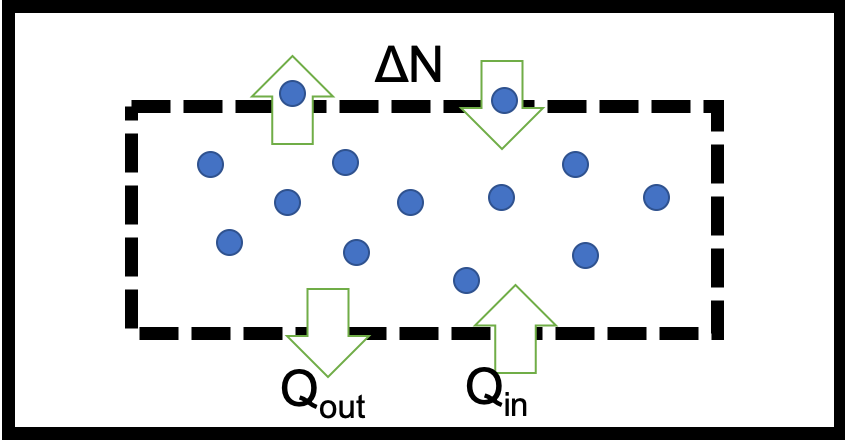
\includegraphics[width=0.45\linewidth]{Methods/plots/grand-canonical-ensemble.png}}
  \caption[Illustration plot of grand canonical ensemble.]{Illustration plot of grand canonical ensemble. Black line shows the universe. Black dashed line confines the ensemble. Blue solid circles are atoms in the system.}
  \label{Chap:Meth:GCMC:fig1}
\end{figure}
\endgroup

\subsection{Monte Carlo Methods}
\label{Chap:Mech:GCMC:MC}

\ac{MC} methods are a broad class of computational algorithms that rely on repeated random sampling to obtain numerical results for a problem that is difficult to solve in principle. The physics behind is to use randomness to solve problems that might be deterministic. They are often used in mathematical \cite{hubbard2009modeling} and physical \cite{bortz1975new} problems. In this thesis, \ac{MC} methods are used to do optimization for complex \ac{GB} structures in Chapter \ref{Chap:Ag/ZnO:GB}, thin-film morphology in Chapter \ref{chap:Ag/ZnO} and solving stochastic time evolution in Chapter \ref{chap:Al/Vac}. A general \ac{MC} algorithm involves: i) drawing a random number $u \in (0,1]$ and ii) accepting/rejecting event base on Boltzmann probability.

\subsection{Grand Canonical Monte Carlo Simulation}
\label{Chap:Mech:GCMC:GCMC}

\ac{GCMC} simulation combines the grand canonical ensemble with \ac{MC} simulations. Following grand canonical($\mu VT$) ensemble discussed above, the number of atoms $N$ in the ensemble can be changed, thus grants two types of events, inserting a new atom and deleting an existing atom. In addition to these two events, moving an atom to a different location is also considered in the event list. Therefore, the probability of accepting moving an existing atom is via \cite{frenkel2001understanding}:
\begin{align}
acc(s \rightarrow s') = \text{min}(1, exp(-\beta(U(s'^N) - U(s^N))
\label{Chap:Meth:eq:acc:move}
\end{align}
inserting a new atom:
\begin{align}
acc(N \rightarrow N+1) = \text{min}(1, \frac{V}{\wedge^3(N+1)}exp(\beta(\mu - U(N + 1) + U(N)))) \label{Chap:Meth:eq:acc:insert}
\end{align}
and removing an existing atom:
\begin{align}
acc(N \rightarrow N-1) = \text{min}(1, \frac{\wedge^3(N)}{V}exp(-\beta(\mu + U(N - 1) - U(N)))) \label{Chap:Meth:eq:acc:remove}
\end{align}
where, $\beta$ is the thermodynamic beta and $\wedge$ is the de Broglie wavelength. Additionally, \ac{MD} steps are usually combined together with \ac{GCMC} simulations to reduce the thermal instability or stress introduced by randomly inserting and moving atoms, as know as the hybird \ac{MC}/\ac{MD} method in Chap. 4.4 of Frenkel 2001 \cite{frenkel2001understanding}. Atomic structures in my thesis are generated by Atomeye, a high efficient visualization tool for millions of atoms. \cite{li2003atomeye}
\section{Kinetic Monte Carlo Simulation}
\label{chap:meth:KMC}

Many real reactions will take a long time, for example, hours, to happen, so the reaction kinetics are difficult to observe by only using \ac{DFT} calculations or \ac{MD}. As discussed in Section \ref{Chap:Mech:GCMC:MC}, \ac{MC} method is used here to help to solve stochastic time evolution in a much longer time scale. Much previous research used this method to simulate vacancy bulk diffusion, surface diffusion, and surface growth. \cite{frenkel2001understanding, leach2001molecular} A typical \ac{kMC} method is shown in Algorithm \ref{algo:kMC}.

\begin{figure}[htb]
\centering
\begin{minipage}{.7\linewidth}
\begin{algorithm}[H]
  \caption{Kinetic Monte Carlo Algorithm}\label{algo:kMC}
  \begin{algorithmic}[1]
    \State Start the simulation at time t = 0.
    \While {$t < t_{Max}$ Or $epoch < epoch_{Max}$}
        \State Build or update an event list for all the possible event i with rate $r_i$ in the system.
        \State Calculate the cumulative rate $R = \sum_{j=1}^N r_j$,
            where $N$ is the total number of events. 
        \State Calculate probability, $p_i$, of event i by normalizing $r_i$ by $R$.
        \State Generate two uniform random number $u, v \in (0, 1]$.
        \State Choose the event $i$ based on,
               $\sum_{k=1}^{i-1} p_k < u < \sum_{k=1}^{i} p_k$.
        \State Carry out the event $i$.
        \State Update the time with $t = t + \Delta t$,
            where $\Delta t$ is obtained via
            \begin{align}
                \Delta t = - \frac{\log{v}}{R_N}
            \label{Chap:Meth:eq:KMC:1}
            \end{align}
    \EndWhile
\end{algorithmic}
\end{algorithm}
\end{minipage}
\end{figure}

For a system of vacancy on-lattice diffusion in bulk materials, each event rate can be calculated from \ac{DFT} with \ac{NEB} method in principle. However, \ac{NEB} calculations are extremely time-consuming for simulating billions of steps for \ac{kMC}. And the relationship between diffusion barriers and energy differences are not linear for multi-component systems. Therefore, the \ac{NN} functional is trained based on \ac{DFT} calculations to predict diffusion barriers. Thus, we can build a multi-scale methodology, which combines \ac{DFT}, \ac{NN}, and \ac{kMC}, to study the thermodynamics and kinetics of the early nucleation stage of GP zone in Al alloys.
\section{Deep Learning and Neural Network}
\label{Chap:Mech:NN}

As previously mentioned in Chapter \ref{Chap:Mech:DFT}, \ac{DFT} calculations are accurate but also computationally costly. In order to solve the short time span of \ac{DFT} simulations, researchers fit \ac{DFT} results to classical force fields or empirical interatomic potentials, which are simpler analytical formulas or functional. Classical force fields or empirical interatomic potentials simplify the description of inter-atomic interactions by summing components of the short-ranged bonding\cite{jones1924determination}, angular\cite{justo1998interatomic}, dihedral\cite{cornell1995second}, and long-ranged Coulomb interaction\cite{liang2013classical}. Empirical potentials can be used in large-scale atomistic simulations with a reduced computational cost. Scientists and researchers have been constantly working on fitting more accurate empirical potentials to improve statistical sampling and accuracy of \ac{MD} and \ac{MC} simulations for the longer time domain. Due to the simplicity of analytical formulas and costly \ac{DFT} calculations, empirical potentials can only focus on a limited number of material properties of the fitted system. As the number of species included in the system increases, it is also more difficult to fit the desired empirical potential. Besides, empirical potentials are, in general, good at describing the interactions close to the equilibrium, but not very well at intermediate or transitional states. Therefore, to study the early nucleation stage of multi-component systems via vacancy diffusion, a more complex functional need to be used, which could be machine learning or \acf{NN} methods.

\begingroup
\begin{figure}[!ht]
  \centering
  \subfigure[]{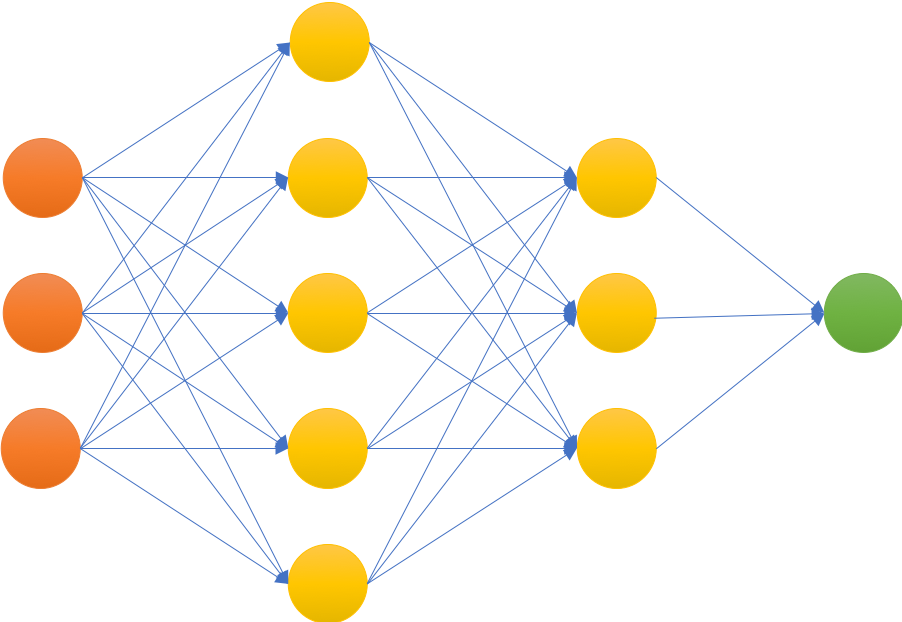
\includegraphics[width=0.9\linewidth]{Methods/plots/nn.png}}
  \caption[Illustration plot of a neural network.]{Illustration plot of a neural network. Orange, yellow, and green nodes indicate the input layer, hidden layers, and output, respectively.}
  \label{Chap:Meth:NN:fig1}
\end{figure}
\endgroup
Recently, machine learning methods have been widely used in materials science to construct the interatomic force fields in complex multi-component systems\cite{artrith2016implementation}, predict material properties\cite{hu2019local,hu2020predicting}.
Deep learning (or \ac{NN}) is a special category of machine learning models that uses a network of neurons, which are arranged in (fully/partially) interconnected layers. A \ac{NN} works similarly to the human brain’s neural connectivity, which will be activated under certain circumstances using various activation functions. \ac{NN}s are non-linear functions with parameters in different layers, called weights. Weights are optimizable through the back-propagation method of a cost function with respect to each weight. The input layer collects input patterns. The output layer has classifications or regression values to which input patterns are related. Hidden layers fine-tune the input weighting parameters until the \ac{NN}’s cost function is minimal. It is hypothesized that hidden layers extrapolate features in the input data that have predictive power about the outputs. In Figure \ref{Chap:Meth:NN:fig1}, a two-layer \ac{NN} is shown. Three orange nodes on the left indicate input nodes, which can be atom species encoding in the on-lattice bulk diffusion model. Yellow nodes in the middle are two layers of fully connected hidden layers. The green node on the right is the output layer, which can be the diffusion barrier. In practice, the neural network architecture will be much more complicated. Details of fitting diffusion barriers will be discussed in Chapter \ref{chap:Al/Vac}.
 
 \chapter{Electronic Mechanism of H Adsorptions on ZnO Surfaces}
 \label{chap:ZnO_H}
 Adsorption strengths of H on anion-terminated (000$\overline{1}$) surfaces of pure and doped wurtzite ZnO are investigated under varying H surface coverage conditions. Consistent with the prediction of the classical electron counting rules, a $\frac{1}{2}$ \ac{ML} of adsorbed H changes the electronic structure of pure ZnO (000$\overline{1}$) surface from metallic to semiconductor state by saturating unpaired electrons of surface oxygen atoms. This closed-shell electron configuration of ZnO (000$\overline{1}$) surface significantly reduces the adsorption strengths of subsequent H atoms, making the dissociative adsorption of a hydrogen molecule endothermic. A simple electron counting model is applied to predict and tune the coverage-dependent H adsorption strengths on general polar semiconductor surfaces. This model is confirmed by our investigations of H adsorption on (000$\overline{1}$) surfaces of ZnO with a series of dopant elements (Na, Mg, Al, Ti, Fe, Sn, etc.). It can also be applied to H adsorption on other similar polar semiconductors, such as ZnO (000$\bar{1}$) containing O vacancies, wurtzite GaN  (000$\overline{1}$), and zincblende ZnS ($\overline{1}$$\overline{1}$$\overline{1}$) surfaces.

\section{Introduction}
\label{ZnO_H/Intro}
H adsorption on solid surfaces is critical to determine the electronic \cite{pearton2010recent,friend1987electronic}, optical \cite{lee2003electrical,major1986effect}, catalytic \cite{xie2011control,haruta1989gold,levy1973platinum} and many other material applications based on surface physical and chemical properties. For example, the catalytic activities of noble metal catalysts depend on the adsorption strength of critical reaction intermediates on noble metal surfaces at steady states \cite{qi2012adsorbate}. The surface electronic structures of oxides, such as ZnO, can change significantly with different surface coverage of H atoms, and there are still debates on whether the origin of the n-type ZnO conductivity results from adsorbed H on ZnO surfaces \cite{janotti2009fundamentals}. In addition, semiconductor oxides are used as the substrate materials for the metallic thin films, whose adhesion strengths on these substrates can be reduced significantly because of adsorbed H on substrate surfaces, resulting in thin-film dewetting and the formation of the undesired discontinued islands \cite{lin2007density,duriau2006growth}.

There have been many theoretical studies based on first-principles calculations to investigate H adsorption on both metal and oxide surfaces.  The adsorption strengths of H and other adsorbates on surfaces depend not only on the interaction between the surface and a single adsorbed atom/molecule but also the lateral interactions between adsorbates. Usually, the lateral interactions are relatively strong for adsorbates with relatively large atomic sizes, such as oxygen (O), hydroxyl (OH) and carbon monoxide (CO) \cite{Miller09,qi2012adsorbate}. It is excepted that H atoms have relatively weak lateral interactions. First-principles calculations confirmed that H adsorption strength increases slightly and continuously when H surface coverage $\theta_{\textup{H}}$ increases from 0 \ac{ML} to 1 \ac{ML} on metal surfaces \cite{pallassana1999theoretical}. Thus, H coverage on metal surfaces at equilibrium conditions change smoothly with H chemical potential in the reservoir, and Langmuir model can be used to describe the adsorption isotherm of H atoms in many circumstances \cite{Benard01}.

On semiconductor surfaces, the coverage-dependent H adsorption strengths may show different characteristics compared to those on metal surfaces. H coverage on these semiconductor surfaces at equilibrium conditions can change discontinuously by varying H chemical potential in the reservoir. Surface phase diagrams of H adsorption are applied to describe the stable surface structure with different H coverage \cite{deWalle02GaN,wang2005hydrogen,lauritsen2011stabilization}. Clean semiconductor surfaces contain unpaired electrons in dangling chemical bonds and can be energetically unstable \cite{Harrison79, dulub2003novel,wander2001stability,hellstrom2017surface,calzolari2013dipolar}. These surfaces can be stabilized by either surface reconstructions or adsorptions under different environmental conditions \cite{Kaxiras87, meyer2004first,lauritsen2011stabilization,wahl2013stabilization,valtiner2009temperature,Jacobs16ZnO}, and the electron counting rule \cite{pashley1989electron} plays an important role. Recently, a simple electron counting model is developed to predict and study the half-Heusler surfaces of CoTiSb \cite{kawasaki2018simple}. Similarly, the electron counting rule can also be applied to H adsorptions on semiconductor surfaces. So far many surface phase diagrams were obtained case-by-case using first-principles calculations. Most of the reported unreconstructed surfaces with lowest energies \cite{meyer2004first,valtiner2009temperature,Jacobs16ZnO} still follow the electron counting rule. Based on the understanding of the electron counting rule, it is easy to predict equilibrium H coverage on a given surface construction. However, a general method to manipulate H surface coverage is still missing.

Many efforts have been made to study H adsorption on surfaces of ZnO \cite{Meyer03,meyer2004first,wang2005hydrogen,valtiner2009temperature,lauritsen2011stabilization, wahl2013stabilization, Jacobs16ZnO}, a wide-band-gap semiconductor widely used in the fields of catalysis, gas sensing, and optoelectronics \cite{Ozgur05_ZnO,Klingshirn07_ZnO}. There are also a few studies on surfaces of ZnO with dopant elements, like Al and Mg \cite{lin2009first, lahmer2015effect}. Since there are increasing applications of doped ZnO and other semiconductors depending on their surface structures and electronic properties \cite{Pan08_doped_ZnO, Georgekutty08_Ag_ZnO, lin2009first, Ling11_Sn-Doped, Buonsanti11_Al_ZnO, Kim14_doped, Hsu14_Ag_ZnO, Lin17_Ni_SnO2}, it is necessary to explore the general principles that guide H adsorption strengths on a wide range of pure and doped ZnO and similar semiconductor surfaces. Especially, it will be interesting to verify for these general cases the accuracy of the electron counting model, which was recently applied to determine the atomic and electronic structures of (001) surface of CoTiSb, a prototypical semiconducting half-Heusler compound \cite{kawasaki2018simple}.

When ZnO bulk structure is chopped into slabs along [0001] directions, two types of surfaces, O-terminated (000$\overline{1}$) surface and Zn-terminated  (0001) surface, are exposed as shown in Fig. \ref{Chap:ZnO_H:fig:ZnO}. These two surfaces were found to have different stabilization principles\cite{lauritsen2011stabilization}: the Zn-terminated  (0001) surface usually has corrugated morphology and complex surface reconstructions because the transition-metal element Zn is more flexible with respect to bonding orientation \cite{dulub2003novel,woll2007chemistry}; the O-terminated (000$\bar{1}$) surface is usually flat on the top layer with different coverage and occupation sites for O and H atoms depending on their chemical potentials because O prefers the bonding configurations with certain bond angles and nearest neighbors \cite{meyer2004first,lauritsen2011stabilization}. In addition, many functional applications of ZnO surfaces are used in oxygen-rich environments, where there are few oxygen vacancies on ZnO (000$\bar{1}$) surface \cite{meyer2004first,lauritsen2011stabilization,wahl2013stabilization}. For these reasons, we use the simple O-terminated (000$\bar{1}$) wurtzite ZnO by its bulk-terminated ideal form (the top surface in Fig. \ref{Chap:ZnO_H:fig:ZnO}) as the model system to investigate the effects of electronic structures and dopant elements on the coverage-dependent H adsorption strength in this study.

\section{Methods}
\label{sec:method}

\begingroup
\begin{figure}[!ht]
  \centering
  \subfigure[]{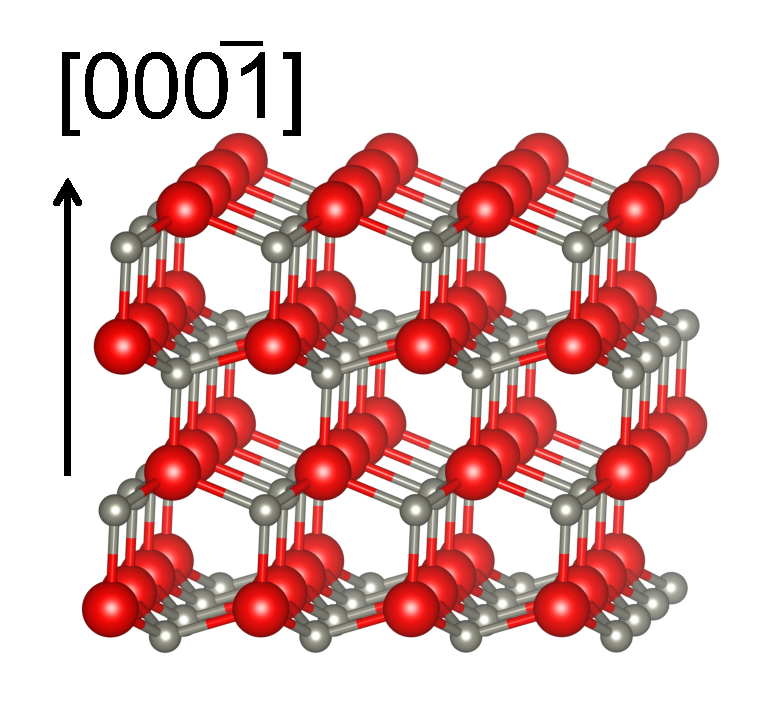
\includegraphics[width=0.4\linewidth]{Chap1/polar1.pdf}}\label{Chap:ZnO_H:fig:ZnO}
  \subfigure[]{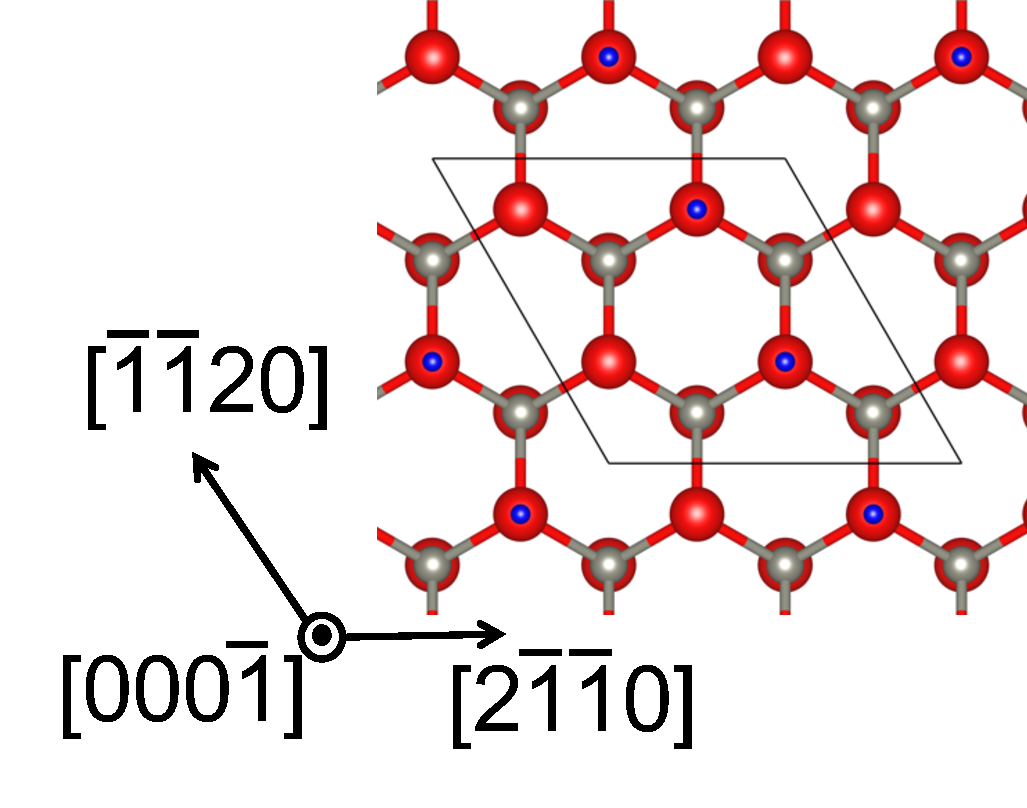
\includegraphics[width=0.4\linewidth]{Chap1/surface2x2.pdf}}\label{Chap:ZnO_H:fig:ZnOSurf}
\caption[Schematic of (2$\times$2) supercell used to model  (000$\bar{1}$) wurtzite ZnO surface with H adsorption.]{(a) and (b): Schematic of (2$\times$2) supercell used to model  (000$\bar{1}$) wurtzite ZnO surface with H adsorption. Large red, small grey and small blue atoms are O, Zn and H atoms, respectively. (a) is the side view projection of ZnO (000$\bar{1}$) slabs, (b) is the top view of (2$\times$2) O-terminated (000$\bar{1}$)  ZnO surface with $\frac{1}{2}$ ML adsorbed H.}
\label{fig1}
\end{figure}
\endgroup

We performed first-principles calculations based on \ac{DFT} by using \ac{VASP} \cite{kresse1996efficient,kresse1999ultrasoft}. Projector augmented wave (PAW) \cite{blochl1994projector} potentials with Perdew-Burke-Ernzerhof (PBE) \cite{perdew1996generalized} exchange-correlation functional and the Hubbard U correction \cite{dudarev1998electron} were used. We applied GGA+U with $U_\text{eff}=U - J = 5.0 eV$ on Zn \textit{d} orbitals as reported in literature\cite{huang2012detailed, oba2010native}. Several other Hubbard U correction parameters ($\text{U}_\text{eff} =$ 3.0 or 7.5 eV) were also tested and showed no significant effects on H adsorption energies. K-points sampling for Brillouin zone integration was performed on a grid of 6$\times$6$\times$1, 6$\times$4$\times$1 with Monkhorst-Pack meshing scheme for (2$\times$2) and (2$\times$3) surface, respectively\cite{monkhorst1976special}. An energy cut-off of 450.0 eV was used in the calculation. The electronic convergence threshold was set as $10^{-4}$ eV. The wurtzite ZnO (000$\overline{1}$) surfaces were constructed by periodic supercell slab models. (2$\times$2) supercells with a vacuum layer of 18 $\angstrom$ in the directions perpendicular to the surfaces were applied as shown in Fig. \ref{Chap:ZnO_H:fig:ZnO} and \ref{Chap:ZnO_H:fig:ZnOSurf}. Each slab contains eight layers of Zn-O repeating units along [0001] direction. Since the ZnO surface slab supercell is not symmetric along [0001] direction, we tested the dipole effects on H adsorption energies and found the dipole effects are minimal if the passivation of the Zn-terminated surface eliminates the artificial electron transfer described as the following. So only the results corresponding no dipole corrections are reported in this study.

As shown in Fig. \ref{Chap:ZnO_H:fig:ZnO}, two types of surfaces are exposed, O-terminated (000$\overline{1}$) surfaces and Zn-terminated  (0001) surfaces, are presented in ZnO slab by its bulk-terminated ideal form. In theoretical modeling, if both sides of a surface slab layer are exposed without modifications, there will be unbalanced electron transfer from Zn-terminated surface to O-terminated surface\cite{Meyer03}. In reality, if the O-terminated surface is exposed to the external environment, the Zn-terminated surface usually is connected to a substrate, which can act as an electron reservoir and compensate unsaturated electrons on the Zn-terminated surface. Many methods have been applied to reduce this artificial electron transfer, such as the introduction of pseudo-hydrogen passivation atoms, Zn vacancies and other adsorbates on Zn-terminated surfaces\cite{calzolari2013dipolar,lin2007microscopic,lahmer2015effect}.

In this work, we focused on O-terminated (000$\overline{1}$) ZnO surface, where H atoms are adsorbed on the top of each surface O atoms as shown in Fig. \ref{Chap:ZnO_H:fig:ZnOSurf}. Zn-terminated (0001) surface on the other side of the slab model was passivated by two different methods to exam their effect on long-distance surface-to-surface electron transfer in the same supercell. First, $\frac{1}{4}$ ML of Zn vacancy was introduced on the top layer of the Zn-terminated surface in a (2$\times$2) supercell. Second, pseudo-hydrogen atoms with different numbers of valence electrons were introduced on the top layer of the Zn-terminated surface. Each Zn atom on the top layer of the Zn-terminated surface was bonded with one pseudo-hydrogen atom, which can have 1.5, 1.0 or 0.5 electrons (denoted as H$_{1.5}$, H$_{1.0}$ and H$_{0.5}$, respectively). In this paper, all the adsorption energy calculations and electronic structure analyses were conducted on the supercells with H$_{1.5}$-passivated Zn-terminated surfaces unless otherwise specified. The reason will be explained and verified in Sec. \ref{subsec:pass}.

\section{Results and Discussions}
\label{sec:results}

\subsection{Coverage-dependent Hydrogen Adsorption Energies on ZnO (000$\bar{1}$) Surface}
\label{subsec:Ead}

In this paper, hydrogen adsorption energy $E_{\textup{ad}}^{\textup{H}}$ with H surface coverage $\theta_{\textup{H}}$ equal to $\frac{n}{m}$ ML is calculated as:
\begin{equation}
  \begin{array}{rcl}
       E_{\textup{ad}}^{\textup{H}}(\theta_{\textup{H}}=\frac{n}{m} \textup{ML})&=&E_{\textup{slab+}n\textup{ H}}-E_{\textup{slab+}(n-1) \textup{ H}}-\frac{1}{2}E_{\textup{H}_{2}}
  \end{array}
  \label{eq1}
\end{equation}
Here $E_{\textup{slab+}n \textup{H}}$ and $E_{\textup{slab+}(n-1) \textup{H}}$ is the total energy of surface slab supercell containing $n$ and $n-1$ adsorbed H atoms, respectively, and $E_{\textup{H}_{2}}$ is the energy of an isolated H$_2$ molecule. The ($x\times y$) surface slab supercell itself contains $m=x\cdot y$ duplicates of (1$\times$1) unit cell of 2D surface lattice, so $m=4$ and $m=6$ for (2$\times$2) and (2$\times$3) slab supercells, respectively. As shown in Fig. \ref{Chap:ZnO_H:fig:Ead}, $E_{\textup{ad}}^{\textup{H}}$ on platinum (Pt) (111) surface only increases slightly with a rising surface H coverage $\theta_{\textup{H}}$ ($\delta E_{\textup{ad}}^{\textup{H}}$ $\sim0.1$ eV when  $\theta_{\textup{H}}$ increases from $\frac{1}{4}$ ML to 1 ML ). On the contrary, $E_{\textup{ad}}^{\textup{H}}$ is highly negative and increases slightly on (2$\times$2) slab supercell of (000$\overline{1}$) ZnO when  $\theta_{\textup{H}}$ = $\frac{1}{4}$ and $\frac{1}{2}$ ML, then $E_{\textup{ad}}^{\textup{H}}$ jumps up suddenly after $\theta_{\textup{H}}$ above $\frac{1}{2}$ ML. 

\begingroup
\begin{figure}[!ht]
  \centering
  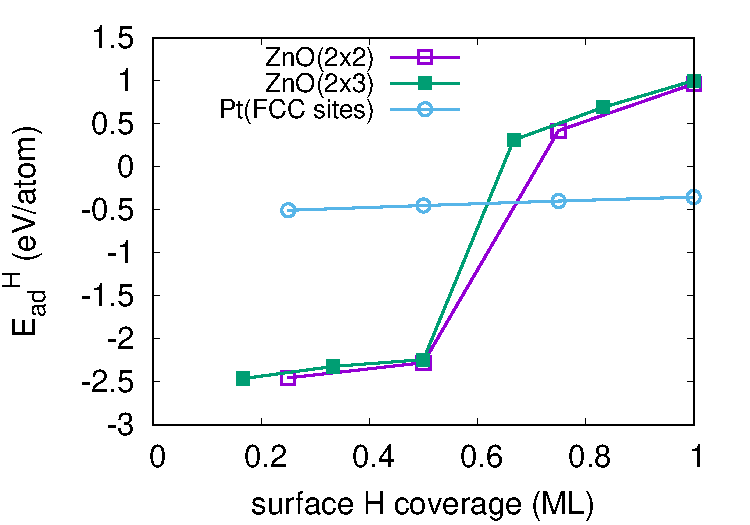
\includegraphics[width=0.75\linewidth]{Chap1/Eadh_coverage_H.pdf}
\caption[H adsorption energies on ZnO surfaces with different H coverage]{H adsorption energies $E_{\textup{ad}}^{\textup{H}}$ defined by Eq. \ref{eq1} on ZnO (000$\overline{1}$) and Pt (111) surfaces with different H coverage}
  \label{Chap:ZnO_H:fig:Ead}
\end{figure}
\endgroup

In order to confirm the critical transition, $E_{\textup{ad}}^{\textup{H}}$ for a larger wurtzite ZnO (000$\overline{1}$) slab supercell with (2$\times$3) in-plane periodicity was also studied. The abrupt increase of $E_{\textup{ad}}^{\textup{H}}$, again, happens when $\theta_{\textup{H}}$ is higher than $\frac{1}{2}$ ML, as shown in Fig. \ref{Chap:ZnO_H:fig:Ead}. It can be concluded that there is a large driving force ($E_{\textup{ad}}^{\textup{H}}$ $<$ -2 eV per H atom) for an isolated H$_2$ molecule to dissociate into two H atoms adsorbed on ZnO (000$\overline{1}$) surface if $\theta_{\textup{H}}$ smaller than $\frac{1}{2}$ ML, above which such adsorption-dissociation reaction becomes highly endothermic and difficult to occur ($E_{\textup{ad}}^{\textup{H}}$ $>$ 0). These results are consistent with previous theoretical calculations and experimental characterizations that $\frac{1}{2}$ ML of adsorbed H were often observed on ZnO (000$\overline{1}$) surface\cite{lin2007density,meyer2004first,lauritsen2011stabilization}.

\subsection{Electronic Structure Analyses and Electron Counting Model}
\label{subsec:electron}

Electronic structures of surface oxygen atoms before and after H adsorption are analyzed in order to understand the mechanism to determine the critical transition of $E_{\textup{ad}}^{\textup{H}}$ on ZnO (000$\overline{1}$) surface. \ac{PDOS} of all four surface O atoms on the top layer of (2$\times$2) ZnO (000$\overline{1}$) surface with different H coverage are plotted in Fig. \ref{Chap:ZnO_H:fig:DOSO}. PDOS of O atoms for $\theta_{\textup{H}}$ = 0 ML and $\frac{1}{4}$ ML cases have strong peaks at the Fermi level, so these ZnO surfaces are in metallic states. When ZnO surface is covered by $\frac{1}{2}$ ML of H atoms, the Fermi level is 0.1 eV above valence band maximum, making these ZnO surfaces in semiconductor states. The cases of  $\theta_{\textup{H}}$ = $\frac{3}{4}$ and 1 ML keep in semiconductor states by further decreasing the valence band maximum to the positions much lower than the Fermi level. PDOS of all surface atoms, including all O, Zn and adsorbed H atoms on the top layer of ZnO (000$\overline{1}$) surface, are plotted in Fig. \ref{Chap:ZnO_H:fig:DOSall} to confirm the above analyses. Similar to Fig. \ref{Chap:ZnO_H:fig:DOSO},  PDOS of all surface atoms for the cases of $\theta_{\textup{H}}$ =  0 ML and $\frac{1}{4}$ ML show strong peaks in the Fermi level, while the PDOS of all surface atoms for the cases of $\theta_{\textup{H}}=\frac{1}{2}$ ML and above exhibit semiconductor characteristics. Thus,  $\frac{1}{2}$ ML is the critical $\theta_{\textup{H}}$ to transform  ZnO (000$\overline{1}$) surface from metallic into semiconductor states. 

\begingroup
\begin{figure}[!ht]
  \centering
  \subfigure[]{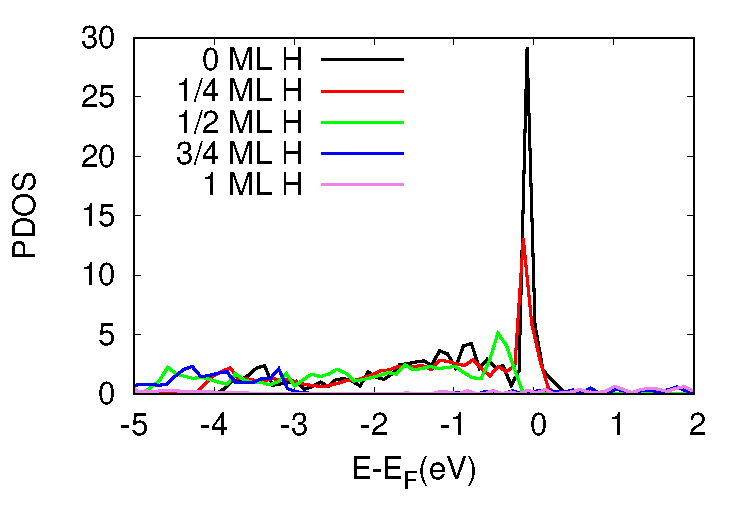
\includegraphics[width=0.45\linewidth]{Chap1/DOS_ZnO_surfO.pdf}}\label{Chap:ZnO_H:fig:DOSO}
  \subfigure[]{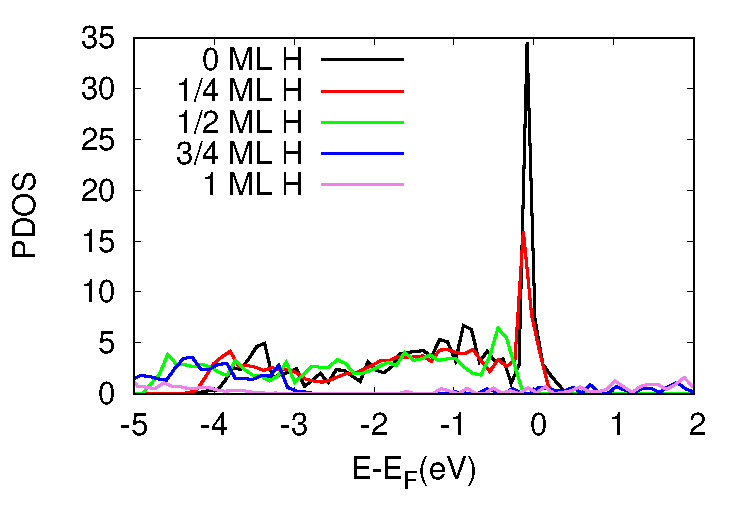
\includegraphics[width=0.45\linewidth]{Chap1/DOS_ZnO_surface_all.pdf}}\label{Chap:ZnO_H:fig:DOSall}
  \caption[PDOS for all the surface O atoms on pure ZnO (2$\times$2) (000$\overline{1}$) surface under different H coverage]{(a) PDOS for all the surface O atoms on pure ZnO (2$\times$2) (000$\overline{1}$) surface under different H coverage. (b) PDOS of all O, Zn and adsorbed H atoms on the topmost layer of ZnO (000$\overline{1}$) surface under different H coverage.}
  \label{Chap:ZnO_H:fig:DOS}
\end{figure}
\endgroup

The coincidence ($\frac{1}{2}$ ML) of the critical $\theta_{\textup{H}}$ for the abrupt change of $E_{\textup{ad}}^{\textup{H}}$ and the critical $\theta_{\textup{H}}$ for the metal-semiconductor transition indicates that $E_{\textup{ad}}^{\textup{H}}$ is controlled by surface electronic structures. This coincidence can be explained by the electron counting model\cite{pashley1989electron}. Each Zn has 2 valence electrons, and each O has 6 valence electrons. In bulk wurtzite lattice, each Zn/O atom connects to 4 nearby O/Zn atoms so that every Zn-O bond has 2 valence electrons, in which 1.5 electrons are contributed from O and 0.5 electron is from Zn. After bulk ZnO is chopped into two slabs with two surfaces in [0001] direction, each surface O and Zn atom has one broken Zn-O bond, as shown in Fig. \ref{Chap:ZnO_H:fig:ZnO}. For Zn-terminated (0001) surface, we applied appropriate methods to passivate the dangling bonds as explained in Sec. \ref{subsec:pass}. For O-terminated (000$\overline{1}$) surface, each O atom requires 0.5 more electron to fill its dangling bond and reach the closed-shell electron configuration. Thus, the electrons of clean O-terminated (000$\overline{1}$) surface are in open-shell configurations. 

The unpaired electrons from surface O atoms are delocalized, making ZnO surface in metallic states. There is a large energetic driving force for surface O atoms to reach closed-shell configurations, meaning ZnO surface has a strong adsorption strength to any atoms/molecules that can contribute electrons to surface O atoms, such as H. In a simple picture, each H atom can contribute one electron to make 2 surface O atoms on (000$\overline{1}$) ZnO surface transform into electron closed-shell configurations. Thus, once $\theta_{\textup{H}}$ reaches $\frac{1}{2}$ ML, there are no unpaired electrons in delocalized states on (000$\overline{1}$) ZnO surface. Correspondingly, the surface transforms into semiconductor state and has much weaker adsorption strength for the consecutive H atoms.

\begingroup
\begin{figure}[!ht]
  \centering
  \subfigure[]{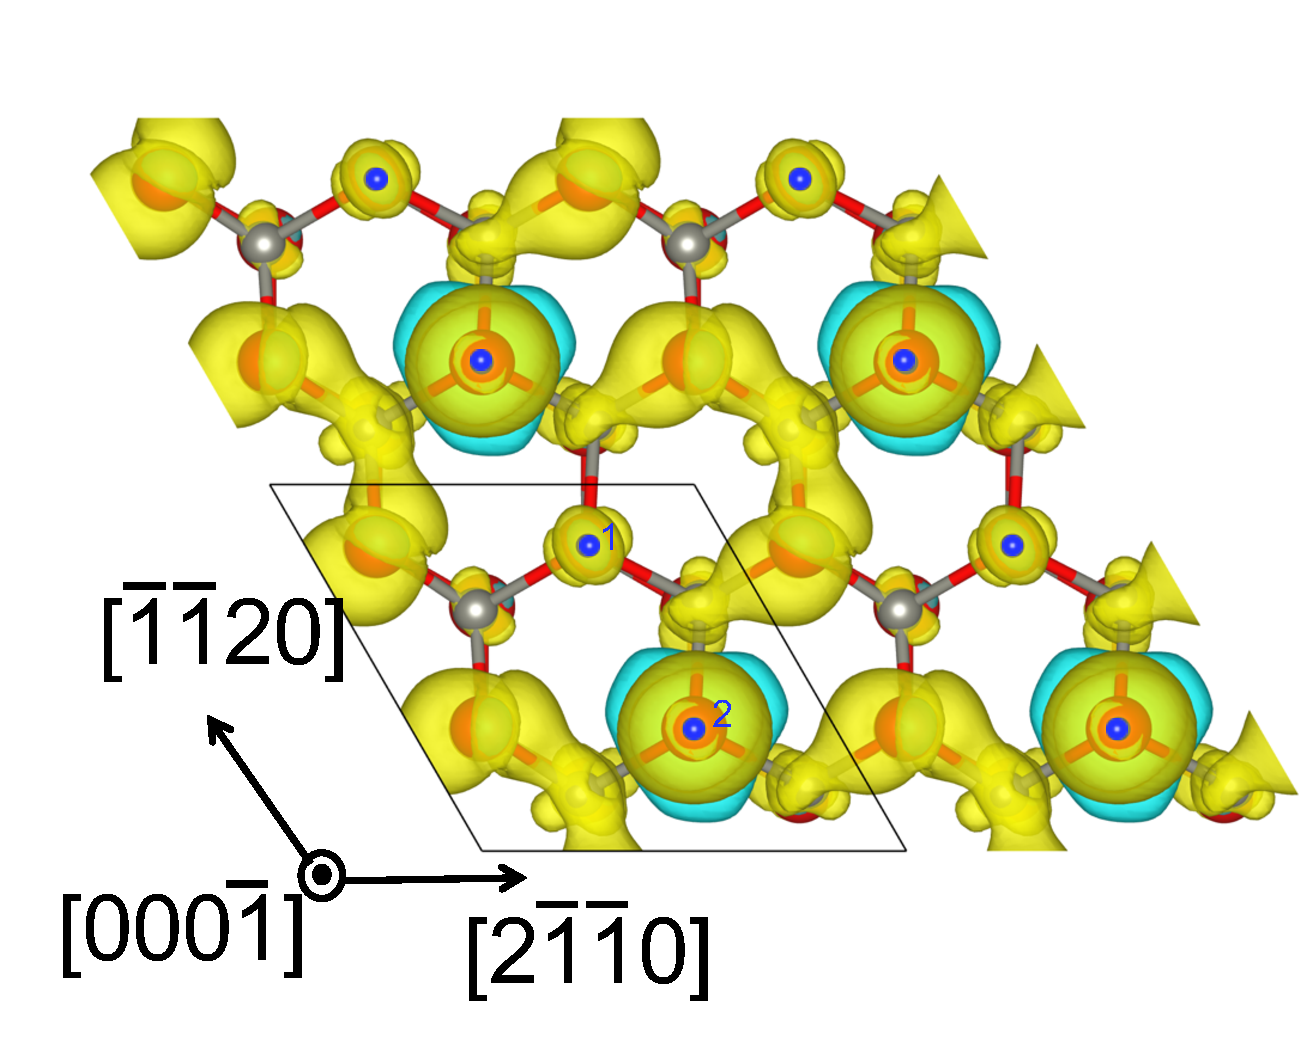
\includegraphics[width=0.49\linewidth]{Chap1/chgdiff1.pdf}}\label{Chap:ZnO_H:fig:chgdiff1}
  \subfigure[]{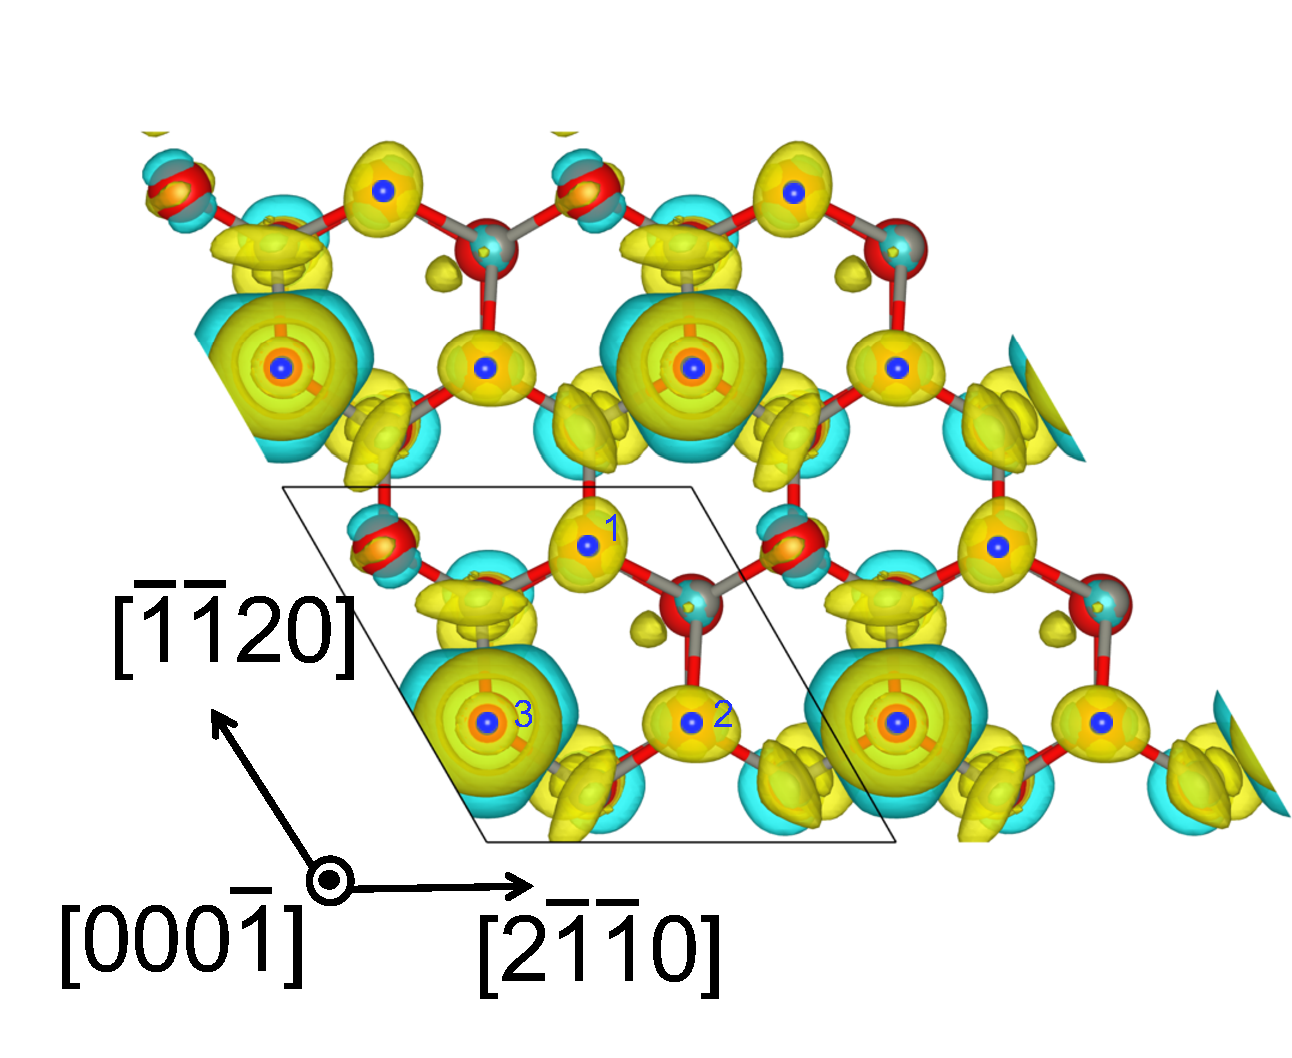
\includegraphics[width=0.49\linewidth]{Chap1/chgdiff2.pdf}}\label{Chap:ZnO_H:fig:chgdiff2}
\caption[Top views of the charge density difference isosurfaces before and after H adsorption]{Top views of the charge density difference isosurfaces before and after (a) the second H and (b) the third adsorption on ZnO (000$\overline{1}$) surface in (2$\times$2) supercells, corresponding to $\Delta\rho(\theta_{\textup{H}}= \frac{1}{2} \textup{ ML})$ and $\Delta\rho(\theta_{\textup{H}}= \frac{3}{4} \textup{ ML})$ defined in Eq. \ref{eq2}, respectively. Large red, small grey and small blue atoms are O, Zn and H atoms, respectively. Label 1, 2 and 3 in the plots denote the adsorption site for the first, second, and third H atom, respectively. The yellow and blue color indicate electron accumulation and annihilation with the isosurface of $0.001e/{\textup{\AA}}^3$.}
  \label{fig3}
\end{figure}
\endgroup

Such electron counting rule and the corresponding PDOS analyses can be further confirmed by the analyses of charge density difference on ZnO (000$\overline{1}$) surface due to H adsorption. Here we define the charge density difference $\Delta\rho$ at different $\theta_{\textup{H}}$ as the following
\begin{equation}
  \begin{array}{rcl}
    \Delta\rho(\theta_{\textup{H}}=\frac{n}{m}\textup{ML})&=&\rho(\textup{slab+}n\textup{H})-\rho(\textup{slab+}(n-1)\textup{H})
  \end{array}
  \label{eq2}
\end{equation}
Here $\rho(\textup{slab+}n \textup{H})$ and $\rho(\textup{slab+}(n-1) \textup{H})$ is the charge density of ZnO (000$\overline{1}$) surface slab with $n$ and $(n-1)$ adsorbed H atoms, respectively. For (2$\times$2) supercell, $\Delta\rho(\theta_{\textup{H}}= \frac{1}{2} \textup{ ML})$ and  $\Delta\rho(\theta_{\textup{H}}= \frac{3}{4} \textup{ ML})$ corresponds to the charge density difference induced by the adsorption of the second and third H atom in the supercell, as shown in Fig. \ref{Chap:ZnO_H:fig:chgdiff1} and  \ref{Chap:ZnO_H:fig:chgdiff2}, respectively. 

In Fig. \ref{Chap:ZnO_H:fig:chgdiff1}, the second H added on (2$\times$2) ZnO (000$\overline{1}$) surface induces charge density accumulation not only near this H atom itself but also other surface sites without H. Such delocalized $\Delta\rho$ is consistent with the metallic state of ZnO (000$\overline{1}$) surface with $\theta_{\textup{H}}$ $<$ $\frac{1}{2}$ ML. The increase of charge density at multiple surface sites indicates that the electron from the second H atom intends to saturate the unpaired electrons on the whole surface and induce the metal-semiconductor transition. In Fig. \ref{Chap:ZnO_H:fig:chgdiff2}, the third H added on (2$\times$2) ZnO (000$\overline{1}$) surface results in charge density accumulation mostly located near the third H atom itself, with a localized s-orbital-like isosurface of $\Delta\rho$ shown in Fig. \ref{Chap:ZnO_H:fig:chgdiff2}. Such localized $\Delta\rho$ is consistent with the semiconductor electronic structure of ZnO (000$\overline{1}$) surface with $\theta_{\textup{H}}$ $\geq$ $\frac{1}{2}$ ML. 

\subsection{Passivation of Zn-terminated ZnO (0001) Surface}
\label{subsec:pass}

As mentioned in Sec. \ref{sec:method}, the above coverage-dependent H adsorption strengths $E_{\textup{ad}}^{\textup{H}}$ on O-terminated (000$\overline{1}$) ZnO surface may change due to different passivation methods on the Zn-terminated (0001) surface, where each Zn atom has a dangling bond with 0.5 unpaired electron in its bulk-terminated ideal form. The dangling bond of each surface Zn atom should be emptied to reach the passivated structure and eliminate the artificial charge transfer from (0001) to (000$\overline{1}$) surface according to the classical electron counting model\cite{pashley1989electron}. It can be achieved by generating a  $\frac{1}{4}$ ML Zn vacancy on (0001) surface layer (one Zn vacancy in the (2$\times$2) supercell) because the 0.5 unpaired electron from each of 3 remaining Zn atoms on (0001) surface can transfer to each of 3 O atoms that are the first-nearest neighbors of the Zn vacancy to form the stable closed-shell electron configurations. In addition, the passivated (0001) surface can also be achieved by adding one atom, such as a pseudo-hydrogen atom with 1.5 electrons (H$_{1.5}$), to each Zn atom on (0001) surface to fill the dangling bond.

\begin{table}[!htbp]
\centering
\caption[Comparison of different passivation mechanisms for the coverage-dependent adsorption energy of H atom]{The coverage-dependent adsorption energy of H atom $E_{\textup{ad}}^{\textup{H}}$ in unit of eV on (2$\times$2) O-terminated (000$\bar{1}$) ZnO surface with different mechanisms to passivate the Zn-terminated (0001) surface, including a clean Zn-terminated surface, a $\frac{1}{4}$ ML Zn vacancy (V$_{\textup{Zn}}$) on the Zn-terminated surface and pseudo-hydrogen atoms with different numbers of valence charges (1.5, 1.0 and 0.5 electron, respectively) at each Zn site on the Zn-terminated surface (H$_{1.5}$, H$_{1.0}$ and H$_{0.5}$).}
\label{tab:pass}
\begin{tabular}{lllll}
\hline
eV/Atom       & 0.25ML & 0.5ML & 0.75ML & 1ML  \\ \hline
V$_{\textup{Zn}}$     & -2.43  & -2.18 & 0.43   & 0.95 \\
H$_{1.5}$         & -2.45  & -2.28 & 0.42   & 0.96 \\
H$_{1.0}$         & -2.45  & -2.27 & 0.11   & 0.95 \\
H$_{0.5}$         & -2.38  & -1.82 & 0.43   & 0.98 \\ 
Clean Zn-terminated & -2.34  & -1.49 & 0.52   & 0.95 \\
\hline
\end{tabular}
\end{table}

Tab.\ref{tab:pass} lists the H adsorption energies on (2$\times$2) (000$\overline{1}$) ZnO calculated using different passivation methods: the addition of Zn vacancies or (pseudo-)hydrogen atoms with different numbers of valence charges (H$_{1.5}$, H$_{1.0}$, and H$_{0.5}$) on (0001) surface. 
$\frac{1}{4}$ ML Zn vacancy (V$_{\textup{Zn}}$) and H$_{1.5}$ generate almost the same $E_{\textup{ad}}^{\textup{H}}$ on (000$\bar{1}$) for all investigated H surface coverages $\theta_{\textup{H}}$. These results confirm that both methods can fully passivated the Zn-terminated surface and eliminate the artificial electron transfer in the supercell. Meanwhile, an obvious difference between  H$_{1.0}$ and H$_{1.5}$ cases can be observed for the adsorption of the third H atom in the (2$\times$2) supercell ($\theta_{\textup{H}}$ = $0.75$ ML), where $E_{\textup{ad}}$ of H$_{1.0}$ case is 0.11 eV, $\sim$ 0.3eV lower than the values for V$_{\textup{Zn}}$ and H$_{1.5}$ cases. This is because one H$_{1.0}$ atom cannot completely fully filled the bonding bond of each Zn atom on (0001). For the cases of Zn-terminated surfaces without pseudo-hydrogen atoms (Clean Zn-terminated in Tab. \ref{tab:pass}) and the cases of H$_{0.5}$, because there are large amounts of electron transfers from Zn-terminated to O-terminated surfaces, H adsorption energies on the O-terminated surfaces are much weaker than those of V$_{\textup{Zn}}$ and H$_{1.5}$ cases for $\theta_{\textup{H}}$ = $0.5$ and $0.75$ ML. Thus, in the paper, only the results corresponding to H$_{1.5}$ cases (fully passivated Zn-terminated surfaces) are reported.

\subsection{Hydrogen Adsorption on (000$\overline{1}$) Surface of ZnO with Dopants}
\label{subsec:doped}

In this study, we find that the electron counting model can also be applied to explain the variation of $E_{\textup{ad}}^{\textup{H}}$ with $\theta_{\textup{H}}$ on (000$\overline{1}$) surfaces of doped ZnO\cite{pashley1989electron}. Different metallic elements are added as substitutional dopants on Zn lattice sites. Because these dopant elements can have different numbers of valence electrons than Zn, it can change the required number of adsorbed H atoms to saturate all surface O atoms and induce the metal-semiconductor transition on the surface. Correspondingly, the critical $\theta_{\textup{H}}$ for the transition of $E_{\textup{ad}}^{\textup{H}}$ can also be varied.  Based on this mechanism, one Zn atom in ZnO bulk lattice is replaced by various types of dopant atoms. 

The dopant atoms located at slab layers with different distances to the top (000$\overline{1}$) surface layer are investigated, and our results show that the location of such dopant atom does not have a significant effect on H adsorption energetics and the critical $\theta_{\textup{H}}$. As illustrated in Tab. \ref{tab:layer}, H adsorption energies with the substitutional dopant elements on Zn lattice sites at different layers away from the O-terminated (000$\bar{1}$) surfaces are listed. H adsorption energies do not show significant variations for the dopant atom at varying distances to the top layer of (000$\bar{1}$) surfaces. Thus, the results for one dopant atom (Al, Ti, V, Na, Mg, Be, Fe, Sn, and Pb) at bulk Zn site far away from the top surface layer in (2$\times$2) ZnO (000$\overline{1}$) supercells are summarized in Fig. \ref{Chap:ZnO_H:fig:doped}. 

\begin{table}[!htbp]
\centering
\caption[Comparison of different doping locations to the top surface layer]{The coverage-dependent adsorption energy of H atom $E_{\textup{ad}}^{\textup{H}}$ (unit: eV/atom) on O-terminated  (000$\bar{1}$) ZnO surface with substitutional Be dopant atom at different locations to the top surface layer. Layer 1 is at the Zn lattice site nearest to the top surface layer.}
\label{tab:layer}
\begin{tabular}{lllll}
\hline
eV/atom      & 0.25ML & 0.5ML & 0.75ML & 1ML  \\ \hline
Layer 1      & -2.71  & -2.39 & 0.52   & 0.97 \\
Layer 2      & -2.38  & -2.23 & 0.43   & 0.97 \\
Layer 3      & -2.42  & -2.28 & 0.51   & 0.94 \\
Layer 4      & -2.39  & -2.32 & 0.46   & 0.98 \\\hline
\end{tabular}
\end{table}

\begingroup
\begin{figure}[!htb]
  \centering
  \subfigure[]{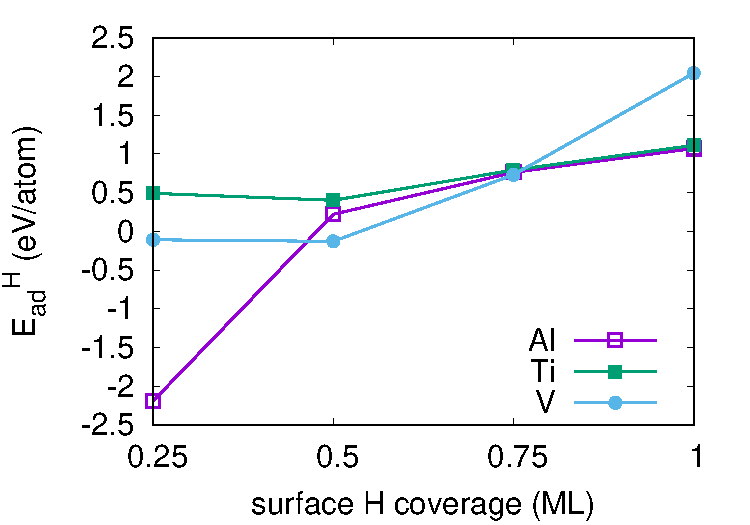
\includegraphics[width=0.32\linewidth]{Chap1/E_C_1.pdf}}\label{Chap:ZnO_H:fig:dop1}
  \subfigure[]{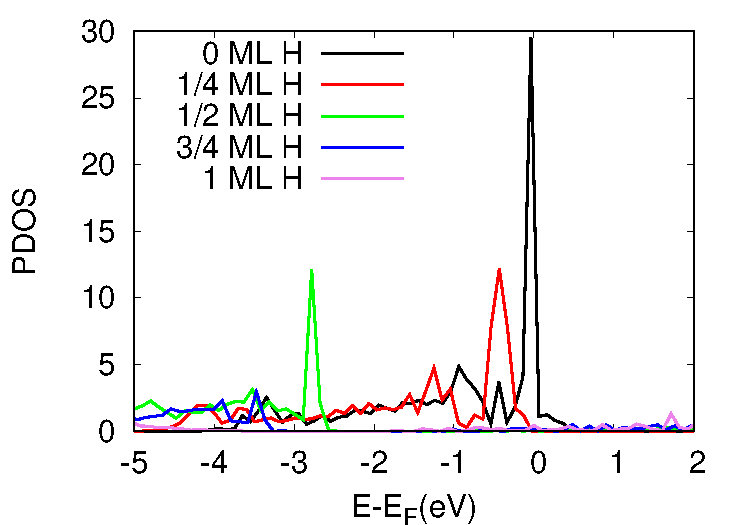
\includegraphics[width=0.32\linewidth]{Chap1/DOS_Al_surfO.pdf}}\label{Chap:ZnO_H:fig:dop2}
  \subfigure[]{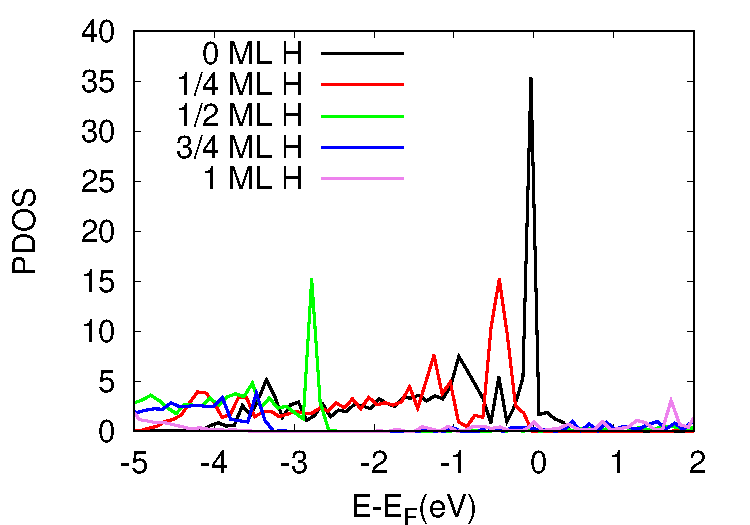
\includegraphics[width=0.32\linewidth]{Chap1/DOS_Al_surf_all.pdf}}\label{Chap:ZnO_H:fig:dop3}
   \qquad
  \subfigure[]{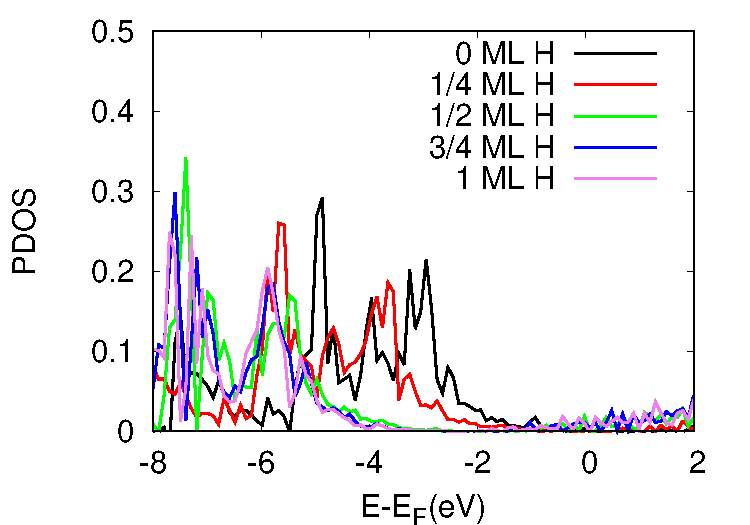
\includegraphics[width=0.32\linewidth]{Chap1/DOS_bulk_Al.pdf}}\label{Chap:ZnO_H:fig:dop4}
  \subfigure[]{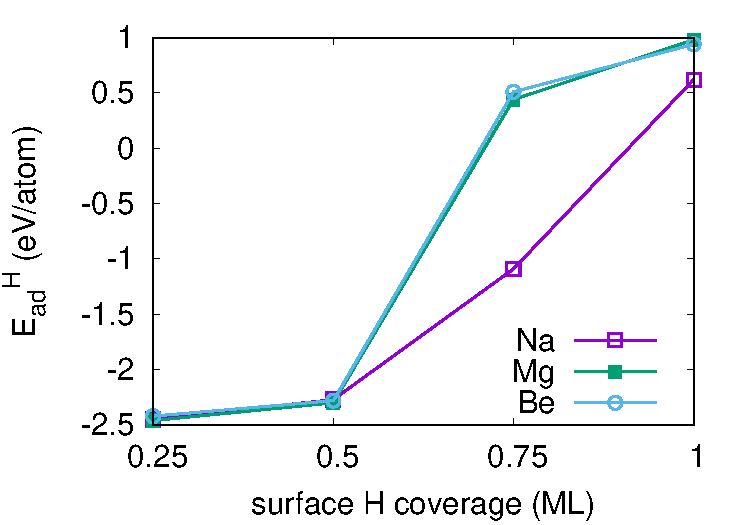
\includegraphics[width=0.32\linewidth]{Chap1/E_C_2.pdf}}\label{Chap:ZnO_H:fig:dop5}
  \subfigure[]{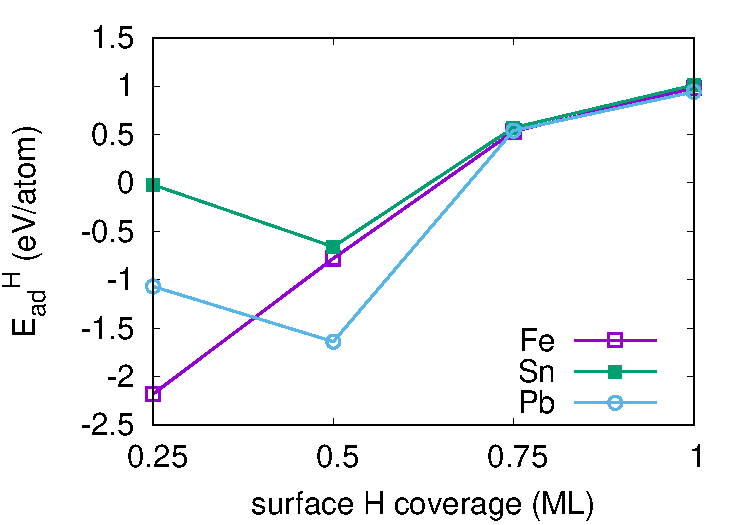
\includegraphics[width=0.32\linewidth]{Chap1/E_C_3.pdf}}\label{Chap:ZnO_H:fig:dop6}
\caption[H adsorptions on ZnO surfaces with different doping]{(a) $E_{\textup{ad}}^{\textup{H}}$ on (2$\times$2) ZnO (000$\overline{1}$) surface with one substitutional dopant atom (Al, Ti or V) at bulk Zn site. Each dopant atom has more valence electrons more than Zn. (b) PDOS for all the O atoms on top surface layer of Al-doped ZnO (000$\overline{1}$) under different $\theta_{\textup{H}}$. (c) PDOS of all O, Zn and adsorbed H atoms on the topmost layer of Al-doped ZnO (000$\overline{1}$) under different $\theta_{\textup{H}}$. (d) PDOS for Al atom in the bulk layer of Al-doped ZnO (000$\overline{1}$) under different $\theta_{\textup{H}}$. (e) $E_{\textup{ad}}^{\textup{H}}$ on (2$\times$2) ZnO (000$\overline{1}$) surface with one substitutional dopant atom (Mg, Be or Na)  at bulk Zn sites. Each dopant atom has equal or less valence electrons than Zn. (f) $E_{\textup{ad}}^{\textup{H}}$ on (2$\times$2) ZnO (000$\overline{1}$) surface with one substitutional dopant atom (Fe, Sn or Pb) at bulk Zn sites. Each dopant atom has multiple common charge states.}
\label{Chap:ZnO_H:fig:doped}
\end{figure}
\endgroup

In Fig. \ref{Chap:ZnO_H:fig:dop1}, all dopant atoms (Al, Ti and V) have more valence electrons than Zn. For Al-doped ZnO surface, if the one extra valence electron from Al already transfers to O atoms on the top surface layer, only one H atom is required to saturate all 4 O atoms in a (2$\times$2) supercell and induce the metal-semiconductor transition according to the electron counting model. Consistent with this interpretation, the H adsorption strength for the Al-doped ZnO surface in Fig. \ref{Chap:ZnO_H:fig:dop1} is as strong as the pure ZnO surface in Fig. \ref{Chap:ZnO_H:fig:Ead} when $\theta_{\textup{H}}$ $\leq$ $\frac{1}{4}$ ML. Above this critical $\theta_{\textup{H}}$, $E_{\textup{ad}}^{\textup{H}}$ suddenly increases to positive values, consistent with the proposed metal-semiconductor transition for ZnO surface. This interpretation is further confirmed by analyses of PDOS of all four surface O atoms on (2$\times$2) Al-doped ZnO surface in Fig. \ref{Chap:ZnO_H:fig:dop2}. PDOS of O atoms with $\theta_{\textup{H}}$ = 0 ML case have strong peaks at the Fermi level. When Al-doped ZnO surfaces are covered by $\frac{1}{4}$ to 1 ML of H atoms, there are no peaks on the Fermi level, making these surfaces in semiconductor states. PDOS of all surface atoms, including all the O, Zn and adsorbed H atoms on the topmost layer of Al-doped ZnO (000$\overline{1}$) surface, are plotted in Fig. \ref{Chap:ZnO_H:fig:dop3} to confirm the above analyses. Similar to Fig. \ref{Chap:ZnO_H:fig:dop2},  PDOS of all surface atoms for the case of $\theta_{\textup{H}}$ =  0 ML  show strong peaks in the Fermi level, while PDOS of all surface atoms for the cases of $\theta_{\textup{H}}=\frac{1}{4}$ ML and above exhibit semiconductor characteristics. PDOS of the Al atom, which is located at the third layer away from the (000$\overline{1}$) O-term surface, under different H surface coverages is also plotted in Fig. \ref{Chap:ZnO_H:fig:dop4}.  As can be seen from the plot, there is no significant peak around Fermi level for all the H surface coverages, showing that the bulk Al atom under different H surface coverages is also saturated in closed-shell electron configuration. Interestingly, PDOS of Al downshifts indicating a stronger bonding between Al and nearby O atoms as the H surface coverages increases.

If one Zn atom is replaced by one Ti or V atom in the (2$\times$2) supercell, because both Ti and V have two or more valence electrons than Zn, all O atoms on (000$\overline{1}$) surface are already saturated without any adsorbed H atoms. Therefore,  both Ti-doped and V-doped ZnO surfaces have very weak H adsorption strengths with $E_{\textup{ad}}^{\textup{H}}$ close to or above zero for all $\theta_{\textup{H}}$ values in Fig. \ref{Chap:ZnO_H:fig:dop1}. Meanwhile, if one Zn atom is replaced by one dopant atom with two valence electrons the same as Zn, such as beryllium (Be) or magnesium (Mg), the variations of $E_{\textup{ad}}^{\textup{H}}$ with $\theta_{\textup{H}}$ are almost the same as those on pure ZnO surface as shown in Fig. \ref{Chap:ZnO_H:fig:dop5}, so the doped ZnO (000$\overline{1}$) surfaces have strong H adsorption strength only when $\theta_{\textup{H}}$ $\leq$ $\frac{1}{2}$ ML. If one Zn atom is replaced by a dopant atom with only one valence electron such as sodium (Na), the dopant can attract one electron from O atoms on (2$\times$2)  (000$\overline{1}$) surface, so three H atoms are required to saturate all 4 O atoms in a (2$\times$2) supercell. Correspondingly, this Na-doped ZnO (000$\overline{1}$) surface has strong H adsorption strength when $\theta_{\textup{H}}$ $\leq$ $\frac{3}{4}$ ML  as shown in Fig. \ref{Chap:ZnO_H:fig:dop5}. 

Moreover, the dopant effects of elements with multiple common charge states are shown in Fig. \ref{Chap:ZnO_H:fig:dop6}. Fe has both +2 and +3 charge states, so the Fe-doped ZnO (000$\overline{1}$) shows H adsorption strengths at the intermediate level between those on Mg-doped and Al-doped ZnO (000$\overline{1}$) surfaces. It only demonstrates strong H adsorption strengths ($E_{\textup{ad}}^{\textup{H}}$ $\ll$ 0 ) only when $\theta_{\textup{H}}$ $\leq$ $\frac{1}{2}$ ML, similar to the cases for Mg dopant, but the adsorption energy of the second H atom ($\theta_{\textup{H}}$ = $\frac{1}{2}$ ML) is much weaker than that of pure ZnO,  similar to the cases for Al dopant. Meanwhile, Sn and Pb elements can have variant charge states ranging from +1 to +4, with +2 and +4 as the most common states\cite{Greenwood97}. Because of the +2 charge state, ZnO (000$\overline{1}$) with either a Sn or Pb dopant atom show very weak H adsorption strengths ($E_{\textup{ad}}^{\textup{H}}$ $\gg$ 0 ) when $\theta_{\textup{H}}$ $>$ $\frac{1}{2}$ ML, similar to the cases for Mg dopant.  However, since each Sn or Pb atom can contribute more than 2 electrons to ZnO (000$\overline{1}$) surface, H adsorption strengths are also significantly weakened when $\theta_{\textup{H}}$ $\leq$ $\frac{1}{2}$ M. In addition, because the +3 charge state is not as stable as +2 or +4 states for Sn/Pb\cite{Greenwood97}, $E_{\textup{ad}}^{\textup{H}}$ of the first H atom ($\theta_{\textup{H}}$ = $\frac{1}{4}$ ML) is even weaker (more positive) than $E_{\textup{ad}}^{\textup{H}}$ of the second H atom ($\theta_{\textup{H}}$ = $\frac{1}{2}$ ML).

\subsection{Hydrogen Adsorption in Generalized Cases and Electron Counting Model}

According to Fig. \ref{Chap:ZnO_H:fig:doped}, in a (2$\times$2) supercell of ZnO (000$\overline{1}$) surface, if one Zn atom is replaced by one metallic dopant atom with 1 (Na), 2 (Mg), 3 (Al) and 4 (Ti) valence electrons, the critical $\theta_{\textup{H}}$ for the metal-semiconductor transition and the abrupt change of $E_{\textup{ad}}^{\textup{H}}$, denoted as  $\theta_{\textup{H}}^{\textup{c}}$, is $\frac{3}{4}$,  $\frac{1}{2}$, $\frac{1}{4}$ and 0 ML, respectively. $\theta_{\textup{H}}^{\textup{c}}$ is simply obtained by the requirement that all O atoms on the top surface layer should be fully saturated in closed-shell electron configuration according to the electron counting model. Thus, $\theta_{\textup{H}}^{\textup{c}}$ can be calculated for other (000$\overline{1}$) surfaces of wurtzite structures, ($\overline{1}$$\overline{1}$$\overline{1}$) surfaces of zincblende structures, and other semiconductor surfaces with two separate sublattices (one for cations and one for anions) and only the anions (O, N, S, etc.) on the top surface layer (\emph{polar semiconductor surfaces}). Generally, with $n_{\textup{dopant}}$ types of dopant elements in bulk lattice, $\theta_{\textup{H}}^{\textup{c}}$ can be calculated in the unit of ML as the following
\begin{equation}
  \begin{array}{rcl}
      \theta_{\textup{H}}^{\textup{c}}&=&(\frac{8}{N_{\textup{bond}}}-\frac{1}{N_{\textup{bond}}}V_{\textup{anion}})\times1.0\textup{ML}\\\\
      &&-\sum_{i=1}^{n_{\textup{dopant}}}\theta_{\textup{dopant}}^i(V_{\textup{dopant}}^i-V_{\textup{cation}})\\
  \end{array}
  \label{eq3}
\end{equation}
Here $V_{\textup{cation}}$, $V_{\textup{anion}}$ and $V_{\textup{dopant}}^i$ is the number of valence electrons for the cation element in bulk lattice, the anion element in bulk lattice and the dopant cation element $i$, respectively. $N_{\textup{bond}}$ is the number of bonds between one cation (anion) and its nearest anion (cation) neighbors in bulk lattice. $\theta_{\textup{dopant}}^i$ is the concentration of the dopant element $i$ per surface area (in unit of ML). For a Al-doped ZnO (000$\overline{1}$) surface that has only one Al atom in a (2$\times$2) supercell, $N_{\textup{bond}}$ = 4, $V_{\textup{cation}}$ = 2, $V_{\textup{anion}}$ = 6, $n_{\textup{dopant}}$ = 1, $V_{\textup{dopant}}^1$ = 3 and $\theta_{\textup{dopant}}^1$ = $\frac{1}{4}$ ML, so $\theta_{\textup{H}}^{\textup{c}}$ = $\frac{1}{4}$ ML according to Eq. \ref{eq3}, consistent with Al-doped result in Fig. \ref{Chap:ZnO_H:fig:dop1}. 

Eq. \ref{eq3} can be easily extended to the cases with multiple dopant elements ($n_{\textup{dopant}} > 1$). For example, if two Zn atoms at bulk Zn substitutional sites are replaced by one Al dopant atom and one Ti dopant atom in a (2$\times$3) supercell of ZnO (000$\overline{1}$) surface, $n_{\textup{dopant}}$ = 2,  $V_{\textup{dopant}}^1$ = 3, $V_{\textup{dopant}}^2$ = 4, and $\theta_{\textup{dopant}}^1$ = $\theta_{\textup{dopant}}^2$ = $\frac{1}{6}$ ML,  so $\theta_{\textup{H}}^{\textup{c}}$ = 0 ML according to Eq. \ref{eq3}. This prediction is confirmed by our calculations of H adsorption strength on this Al-Ti-doped ZnO (000$\overline{1}$) surface shown in Fig. \ref{Chap:ZnO_H:fig:2dop}. 

Eq. \ref{eq3} can also be easily extended to the cases of other defects such as vacancies. For example, recently it was reported that a stable ZnO (000$\overline{1}$) surface configuration has $\frac{1}{3}$ ML Zn vacancies and 10 H atoms in a (3$\times$3) (000$\overline{1}$) surface unit cell \cite{Jacobs16ZnO}. Here the Zn vacancy can be regarded as a type of dopant cation with zero valence electron. Using the corresponding parameters ($N_{\textup{bond}}$ = 4,$V_{\textup{anion}}$ = 6, $n_{\textup{dopant}}$ = 1, $\theta_{\textup{dopant}}$ = $\frac{1}{3}$ ML, $V_{\textup{dopant}}$ = 0 and $V_{\textup{cation}}$ = 2), $\theta_{\textup{H}}^{\textup{c}}$ = $\frac{7}{6}$ ML according to Eq. \ref{eq3}, corresponding to 10.5 H atoms in a (3$\times$3) ZnO (000$\overline{1}$) surface unit cell. It means the adsorption of the 11th H atom in this unit cell would be too weak to occur under normal environment conditions, consistent with the experimental observations and \ac{DFT} calculations \cite{Jacobs16ZnO}.

\begingroup
\begin{figure}[!ht]
  \centering
  \subfigure[]{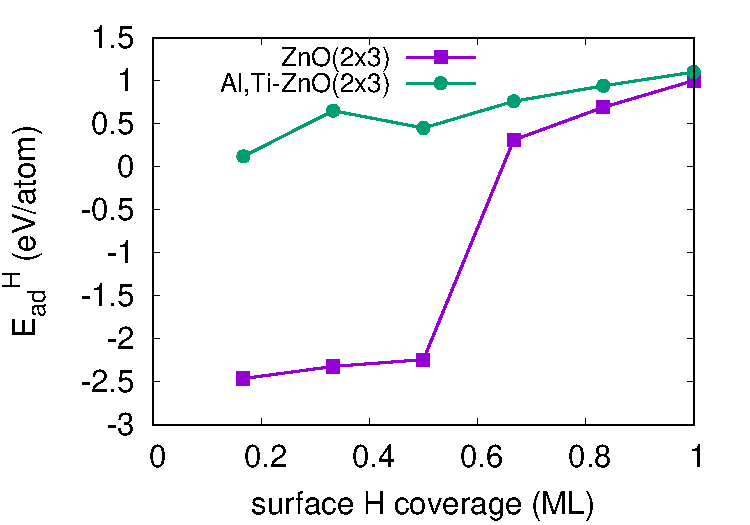
\includegraphics[width=0.45\linewidth]{Chap1/Eadh_2x3_H.pdf}}\label{Chap:ZnO_H:fig:2dop}
  \subfigure[]{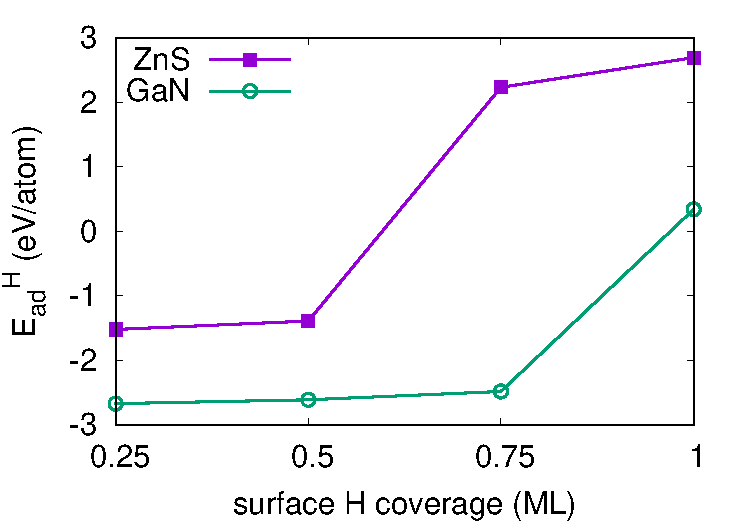
\includegraphics[width=0.45\linewidth]{Chap1/E_C_4.pdf}}\label{Chap:ZnO_H:fig:otherads}
\caption{(e) $E_{\textup{ad}}^{\textup{H}}$ on (2$\times$3) ZnO (000$\overline{1}$) surface with the co-existence of 1 Al substitutional dopant atom and 1 Ti substitutional dopant atom at bulk Zn sites. (a):$E_{\textup{ad}}^{\textup{H}}$ on (2$\times$2) zincblende ZnS ($\overline{1}$$\overline{1}$$\overline{1}$) and wurtzite GaN (000$\overline{1}$) surfaces with different $\theta_{\textup{H}}$. }
  \label{Chap:ZnO_H:fig:others}
\end{figure}
\endgroup

The electron counting model and Eq. \ref{eq3} can be used to explain the H adsorption strength on other polar semiconductor surfaces. For example, sulfur(S)-terminated ($\overline{1}$$\overline{1}$$\overline{1}$) surface of zincblende ZnS have the similar atomistic structure and valence electron configuration as those for wurtzite ZnO (000$\overline{1}$). As shown in Fig. \ref{Chap:ZnO_H:fig:otherads}, the dramatic decrease of H adsorption strength happens when $\theta_{\textup{H}}$ increases from $\frac{1}{2}$ to $\frac{3}{4}$ ML, the same as ZnO in Fig. \ref{Chap:ZnO_H:fig:Ead}. Moreover, for nitrogen(N)-terminated (000$\overline{1}$) surface of wurtzite GaN, because each N atom has 5 valence electrons and 4 Ga-N bonds, $\frac{8-5}{4}$ = 0.75 electron is required to saturate each N atom on (000$\overline{1}$) surface once the GaN bulk lattice is chopped into two surfaces along [0001] direction. According to Eq. \ref{eq3}, $N_{\textup{bond}}$ = 4, $V_{\textup{anion}}$ = 5, and $\theta_{\textup{dopant}}^i$ = 0 ML, so $\theta_{\textup{H}}^{\textup{c}}$ = $\frac{3}{4}$ ML . Therefore, $\theta_{\textup{H}}$ = $\frac{3}{4}$ ML, equivalent to 3 hydrogen atoms in the supercell of a (2$\times$2) GaN (000$\overline{1}$) surface, can transform all 4 surface N atoms from metallic to semiconductor states. Correspondingly, the hydrogen adsorption strength decreases dramatically when $\theta_{\textup{H}}$ increases from $\frac{3}{4}$ to 1 ML as shown in Fig. \ref{Chap:ZnO_H:fig:otherads}. 

\section{Conclusions}
\label{sec:con}

In summary,  the coverage-dependent adsorption of hydrogen atoms on O-terminated (000$\overline{1}$) surface of wurtzite ZnO and other similar polar semiconductor surfaces behave differently than the counterparts on typical metal/alloy surfaces, where H adsorption strength usually decreases slightly and continuously (more positive values of $E_{\textup{ad}}^{\textup{H}}$ in Fig. \ref{Chap:ZnO_H:fig:Ead} ) with increasing H surface coverage \cite{pallassana1999theoretical,qi2012adsorbate}. The adsorption strength of individual H atom on these semiconductor surfaces strongly depends on hydrogen coverage and surface electronic structures. If the surface is in the metallic state, the hydrogen adsorption strength is so strong that the adsorption-dissociation reaction of a single H$_2$ molecule on this surface is highly exothermic at zero K ($E_{\textup{ad}}^{\textup{H}} < -2.0 $ eV in Eq. \ref{eq1}). If the surface is in semiconductor state, the hydrogen adsorption strength is so weak that the adsorption-dissociation reaction of a single H$_2$ molecule on this surface is endothermic at zero K ($E_{\textup{ad}}^{\textup{H}} > 0 $ in Eq. \ref{eq1}).  The surface can be transformed from metallic to semiconductor state by either hydrogen adsorption on the surface or dopant elements in bulk lattice in order to saturate unpaired electrons of anion elements on the top surface layer. The critical H surface coverage $\theta_{\textup{H}}^{\textup{c}}$ to induce such metal-semiconductor transition, which is also the equilibrium H coverage at many experimental conditions \cite{lin2007density,meyer2004first,lauritsen2011stabilization},  is determined by the classical electron counting model described in Eq. \ref{eq3} \cite{pashley1989electron}. This model is confirmed by our investigations of H adsorption on (000$\overline{1}$) surfaces of ZnO with a series of doping elements (Na, Mg, Al, Ti, Fe, Sn, etc.). When doping elements (such as Be, Mg, Na) have equal or less valence electrons than Zn, the critical H coverage will remain unchanged or increase to higher coverages. When doping elements (such as Al, Ti and V) have more valence electrons than Zn, the critical H coverage will decrease to lower coverages. When doping elements (such as Fe, Sn and Pb) have multiple common charge states, the behavior of the critical H coverage will become sophisticated but still follows the general electron counting rule.

This simple electron counting model can be applied to determine and manipulate the equilibrium surface adsorption configurations for H and other adsorbates on different semiconductor polar surfaces with chemical dopant elements. It is different than the d-band model that is widely used to understand trends of H adsorption strengths on different transition metal surfaces \cite{HAMMER95,Kibler05}. Since the driving force for surface reconstruction is also from the tendency to eliminate unpaired electrons and dangling bonds, the model can be used to identify the possible adsorbate and dopant configurations to obtain stable semiconductor surface structures \cite{Kaxiras87,pashley1989electron, Jacobs16ZnO}. It also suggests that the investigations of further adsorptions and depositions of other materials on these semiconductor surfaces should consider the coexistence of adsorbed H atoms at stable configurations. For example,  in many optoelectronic applications, ZnO and other semiconductor oxides are used as the substrate materials for metallic thin films, whose adhesion strengths on these substrates can be reduced significantly because of adsorbed H on substrate surfaces, resulting in thin-film dewetting and the formation of the undesired discontinued islands \cite{lin2007density,duriau2006growth}. Studies in this paper provide a critical step to understand the substrate surface structures and adsorption characteristics for the further investigations on thin film qualities and optoelectronic properties.
 
%  \chapter{Alloy Segregations in Ag Grain Boundaries}
%  \label{chap:Ag_W}
%  
\section{Introduction}
Solute atoms, whether they are added voluntarily for specific needs, inevitably remained as impurities after the synthesis, or introduced during the materials service, can affect various properties of alloys by changing the stability and mobility of crystalline defects.
 
 \chapter{Using Alloy to Enhance Corrosion Resistance of Mg Alloy with Transition Metal Impurities}
 \label{chap:Mg_H}
 In this chapter, we focus on the Mg alloy corrosion due to impurities from casting processing and create a build-in corrosion-resistant mechanism by high-throughput first-principles calculations. A significant challenge for applications of Mg alloys is their poor corrosion resistance and hence Mg alloys designs with built-in corrosion resistance are of significant interest. Corrosion can result from the coupling of anodic dissolution of Mg and cathodic reduction of water on impurities such as Iron (Fe)-rich second-phase particles. Experiments have shown that small quantities of Arsenic (As) or Germanium (Ge) can inhibit Mg corrosion, possibly slowing the \ac{HER} as the cathodic reaction on Fe surfaces. Since a broader experimental search across the periodic table for other Mg corrosion inhibiting elements is unavailable, we designed thermodynamic and \ac{HER} criteria and used high-throughput computations to search a pool of 68 elements including As and Ge that can segregate from bulk Mg to surfaces of Fe particles and impede \ac{HER} there. Our computational procedure predicts that six p-block elements meet these criteria, and they rank according to their ability to reduce H adsorption energies and the \ac{HER} rate as follows: $\text{As} > \text{Ge} > \text{Si} > \text{Ga} > \text{P} \approx \text{Al}$. Results for As, the most effective corrosion-inhibiting element, and Ge are in qualitative accord with recent experiments. While none of the 68 elements was found to enhance H adsorption, the six p-block elements reduce H adsorption via strong orbital overlap (Pauli repulsion) between their outer-shell orbitals and the s orbitals of H adsorbates. These p-block elements are also found to have the potential to reduce \ac{HER} on surfaces of Ni second-phase particles in Mg according to the same criteria, but not on surfaces of Cu second-phase particles. 

\section{Introduction}

\begingroup
\begin{figure}[!ht]
  \centering
  \subfigure[]{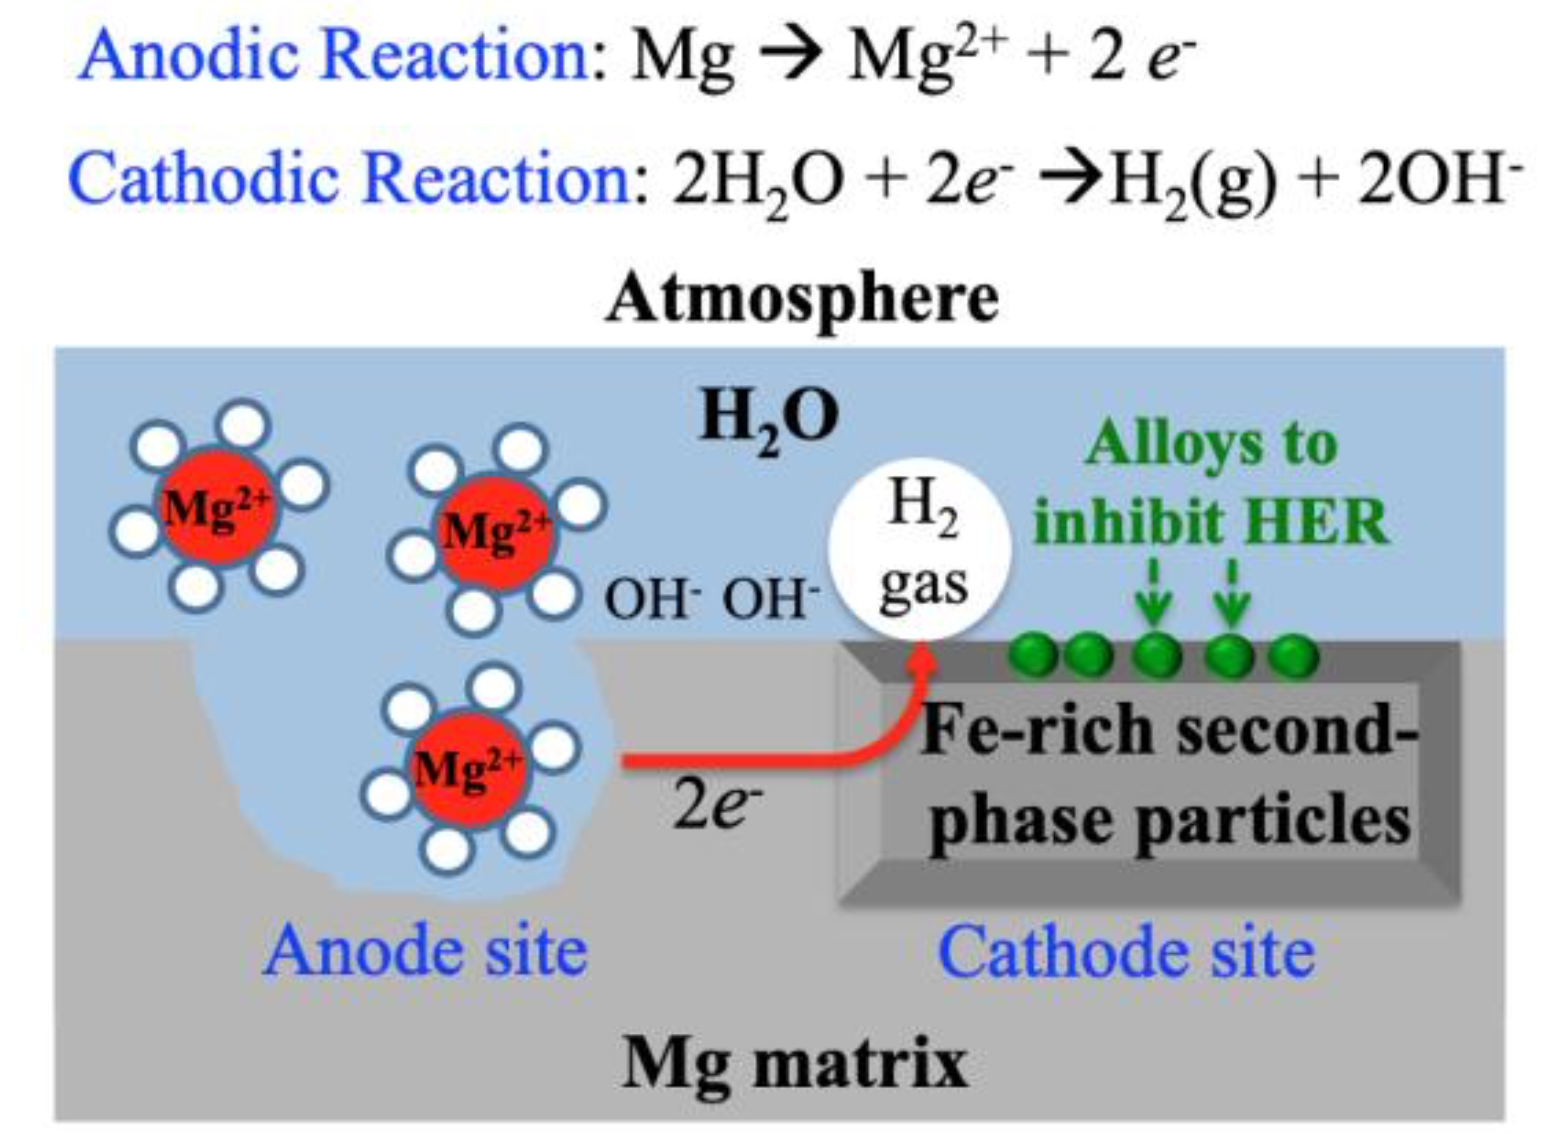
\includegraphics[width=0.49\linewidth]{Chap3/plots/Fig1a.png}}\label{Chap:Mg_H:fig:1a}
  \subfigure[]{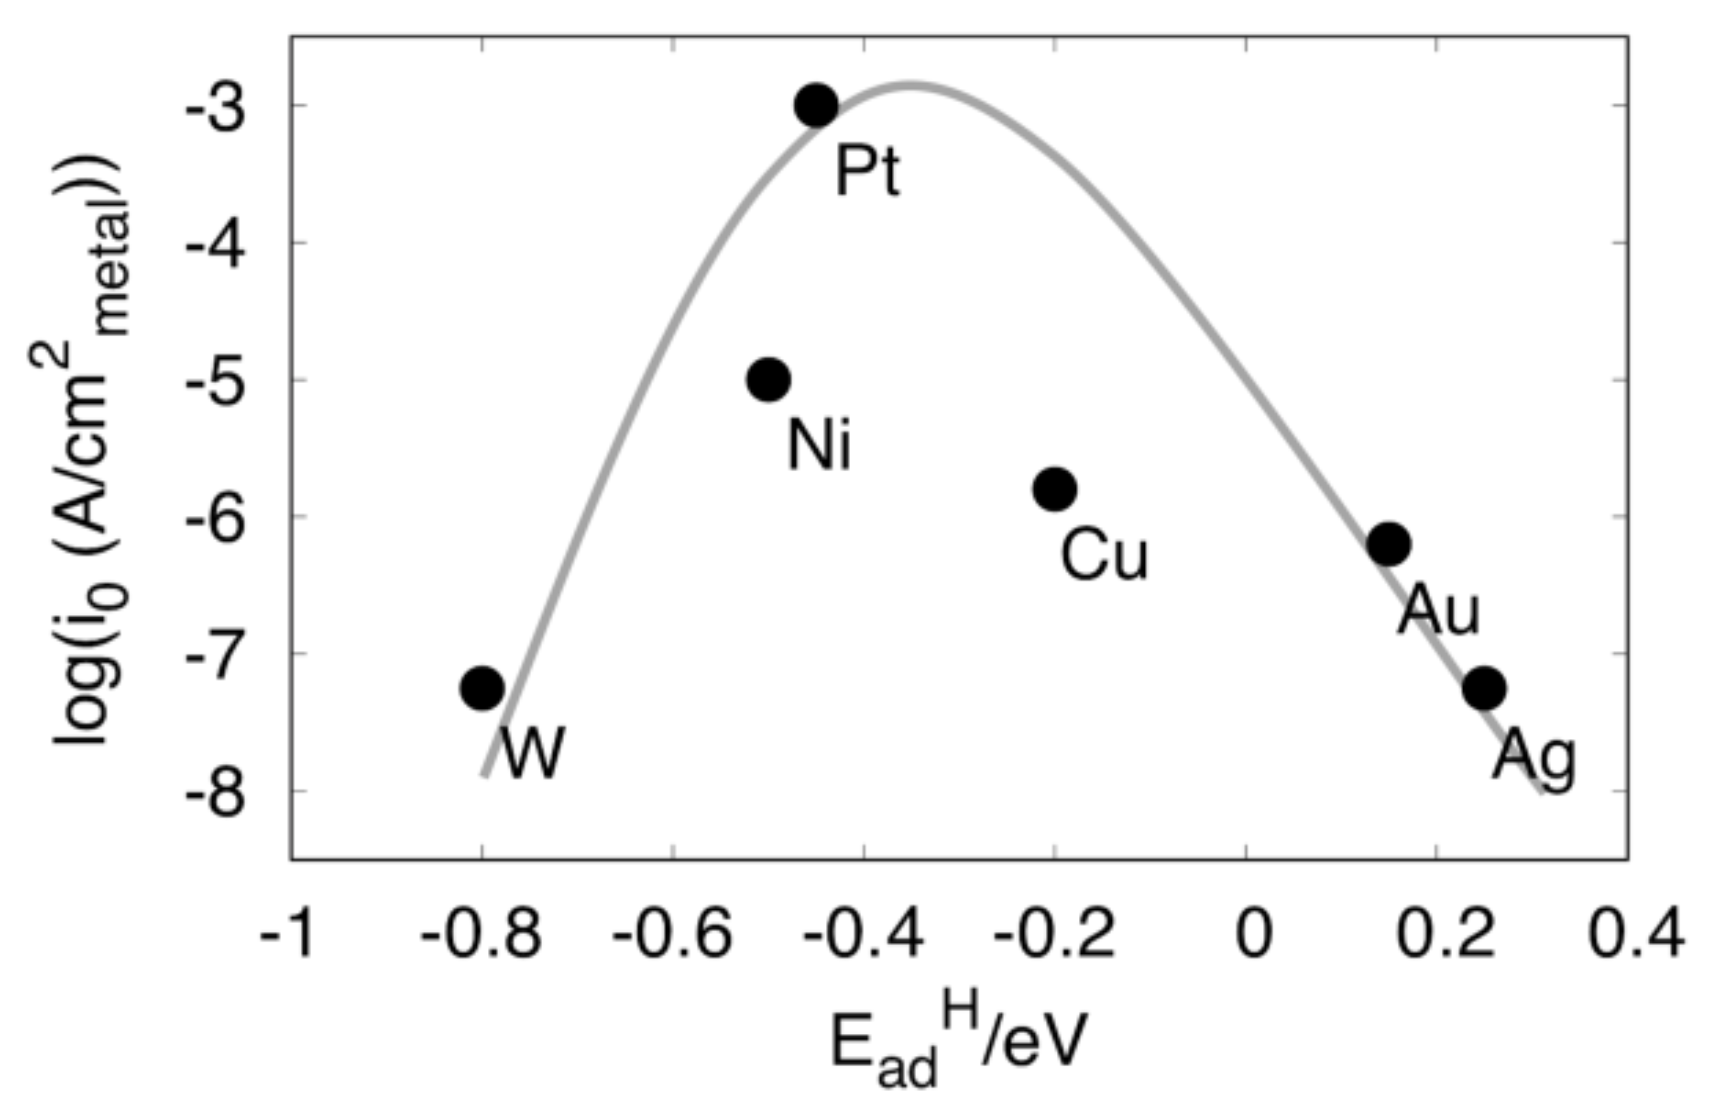
\includegraphics[width=0.49\linewidth]{Chap3/plots/Fig1b.png}}\label{Chap:Mg_H:fig:1b}
\caption[Illustration of corrosion reaction mechanism on Mg and the alloying strategy to inhibit \ac{HER}]{(a) Illustration of corrosion reaction mechanism on Mg and the alloying strategy to inhibit the \ac{HER} as the cathodic reaction. The anodic reaction occurs to Mg matrix by dissolving one Mg atom to produce a $Mg^{2+}$ cation into the electrolyte and two electrons for HER as the cathodic reaction, which occurs on surfaces of second-phase particles, usually rich in Fe and other transition metal elements, to produce a H2 gas molecule. A possible strategy to reduce \ac{HER} rate is to change the H adsorption energy on the surfaces of second-phase particles by proper alloying. (b) Exchange current density of \ac{HER}, $\log(i_0(A/cm^2_{metal})])$, measured in experiments under pH$=$12 vs. H adsorption energy $E_{ad}^H$ defined by Eq. \ref{Chap:Mg_H:eq:H_ads} from \ac{DFT} calculations. This figure is adapted from data of Sheng et al.\cite{sheng2013correlating}. A higher exchange current density corresponds to a faster \ac{HER} and higher corrosion rate. The volcano-shaped solid curve line is plotted only for an illustration the relation between $\log(i_0)$ and $E_{ad}^H$ without quantitative accuracy.}
  \label{Chap:Mg_H:fig1}
\end{figure}
\endgroup

Magnesium alloys are potential candidates for lightweight structural components in transportation industries and other applications due to their low density and high specific strength. Substantial effort has been focused on exploring cast and wrought magnesium (Mg) alloys for application in vehicle propulsion systems and body structures, for example, as part of light-weighting strategies \cite{luo2005development, luo2006wrought,carter2011structural, jekl2015development, luo2013magnesium}. However, corrosion in aqueous and atmospheric environments is one of two significant challenges facing broader implementation of current Mg alloys in vehicles. The other challenge is poor room temperature formability of Mg sheet alloys in stamping, a consequence of the anisotropy in plasticity response associated with the various dislocation slip systems in the \ac{HCP} structure \cite{yasi2010first}. Post-forming surface treatments can be applied to mitigate Mg corrosion \cite{zheng2005corrosion}. 
In an aqueous environment, the coupling between regions of anodic dissolution of Mg and cathodic reduction of water drives galvanic corrosion leading to the removal of Mg and the formation of pits surrounding second-phase particles as cathode sites \cite{birbilis2014evidence, zeng2006review}. Magnesium has a highly negative standard electrode potential of -2.37 V relative to the \ac{SHE}, making it a very active anode (all electrode potential values are relative to the \ac{SHE} in this paper). Anodic dissolution of Mg via 
\begin{align}
Mg \rightarrow Mg^{2+} + 2e^{-}
 \label{Chap:Mg_H:eq:anodic_dissolution}
\end{align}
couples with the cathodic reaction, which is the reduction of water in an alkaline electrolyte 
\begin{align}
2H_2O + 2e^{-} \rightarrow H_{2}(g) + 2OH^{-}
 \label{Chap:Mg_H:eq:cathodic_reaction}
\end{align}
Eq. \ref{Chap:Mg_H:eq:cathodic_reaction} is the \ac{HER} with a standard electrode potential of -0.828 V relative to \ac{SHE}. The overall reaction mechanism is illustrated in Fig. \ref{Chap:Mg_H:fig:1a}. 

Corrosion on Mg proceeds without any limitation for pH < 11 since oxygen is not involved and no passivating surface layer forms \cite{liu2016controlling,ralston2012effect}. Previously, it was found that Fe, Cu, Co and Ni accelerate Mg corrosion in aqueous environments containing chlorides \cite{hanawalt1942corrosion, mcnulty1942some}. Even though Fe (an impurity often introduced during alloy processing \cite{yang2015corrosion, scharf2007iron}) has a very low solubility limit in Mg \cite{mcnulty1942some}, Fe particles in \ac{BCC} structure have been identified as cathode sites. This was demonstrated by Taub et al. \cite{taub2002mechanism} with experiments involving powdered Mg and Fe in chloride solutions. Cathodic reaction in Mg alloys typically occurs at submicron and micron-scale Fe (and Fe-rich) second-phase particles positioned at the metal-aqueous solution interface \cite{yang2015corrosion, eaves2012inhibition}. The detailed roles of Fe-rich particles as cathodic reaction sites can vary according to corrosion potentials (such as the \ac{NDE}) and the populations/sizes of Fe-rich particles \cite{hoche2016effect, yang2018effect}; the cathodic reaction rates should also depend on the surface configurations of Mg, which typically contain mixtures of porous Mg hydroxides and oxides (e.g. aluminum oxide). Hence, the accurate locations of Fe-rich particles relative to these mixtures can result in changes in corrosion rates \cite{taheri2012analysis, taheri2014towards}. Song and Atrens provided an overview of galvanic as well as other corrosion mechanisms of Mg with some useful insights \cite{song2003understanding}. Esmaily et al. presented a comprehensive summary of the recent progress of studies in Mg-alloy corrosion \cite{esmaily2017fundamentals}. 

There is significant interest in designing Mg alloys that have a “built-in” corrosion inhibition mechanism \cite{eaves2012inhibition}. A possible strategy is to slow down the HER rates on cathode sites such as Fe particles in \ac{BCC} phase. The HER can be completed through either the Volmer-Heyrovsky mechanism or the Volmer-Tafel mechanism \cite{ghali2010corrosion,walling1968electrochemical}. The associated reactions are
\begin{subequations}
\begin{align}
&\text{Volmer reaction:    } & H_2O + e^- & \rightarrow H^* + OH^-
 \label{Chap:Mg_H:eq:Volmer}\\
&\text{Heyrovsky reaction:    } & H^* + H_2O + e^- & \rightarrow H_2(g) + OH^-
 \label{Chap:Mg_H:eq:Heyrovsky}\\
&\text{Tafer reaction:    } 
& 2H^* & \rightarrow H_2(g)
 \label{Chap:Mg_H:eq:Tafel}
\end{align}
\end{subequations}
Here * means the corresponding atom/molecule is adsorbed on cathode surface sites. The Volmer-Heyrovsky mechanism proceeds first via Eq. \ref{Chap:Mg_H:eq:Volmer} followed by Eq. \ref{Chap:Mg_H:eq:Heyrovsky}. The Volmer-Tafel mechanism involves Eq. \ref{Chap:Mg_H:eq:Volmer} twice followed by Eq. \ref{Chap:Mg_H:eq:Tafel}. The equilibrium potentials of Eqs. \ref{Chap:Mg_H:eq:Volmer}, \ref{Chap:Mg_H:eq:Heyrovsky} and \ref{Chap:Mg_H:eq:Tafel} depend on the free energies of hydrogen atoms adsorbed on cathode surface sites. 

The slowing down of the HER as the cathodic reaction requires the reduction of reaction rates via the Volmer-Heyrovsky mechanism and the Volmer-Tafel mechanism. Regarding the Volmer reaction in Eq. \ref{Chap:Mg_H:eq:Volmer}, its fast kinetics favors the strong adsorption of an H atom on a cathode surface site to increase its thermodynamic driving force since H* is its reaction product. However, the fast kinetics of the Heyrovsky and Tafel reactions in Eq. \ref{Chap:Mg_H:eq:Heyrovsky} and \ref{Chap:Mg_H:eq:Tafel}, respectively, require the weak adsorption of an H atom since H* is the reactant on the left side of each equation. Thus, the adsorption strength of H atoms on a cathode surface must be at an intermediate range to reach the maximum \ac{HER} rate: this is the Sabatier principle \cite{medford2015sabatier}. Fig. \ref{Chap:Mg_H:fig:1b} shows the exchange-current density of the \ac{HER} vs. H adsorption energy, $E_{ad}^H$, in alkaline electrolytes \cite{sheng2013correlating}: the highest values of $\log(i_0)$ corresponding to the fastest \ac{HER} rate appear for the intermediate $E_{ad}^H$. Similar plots of \ac{HER} rate in acid electrolyte vs. $E_{ad}^H$ have been explored on different metals, even though the detailed reaction mechanisms in the \ac{HER} differ from those in an acid electrolyte. Therefore, to slow down the overall \ac{HER} rate on cathode sites, either the adsorption strength of H must be strongly enhanced, so that the rate of the Heyrovsky and Tafel reactions is largely decreased, or the adsorption of H must be significantly weakened thereby reducing the rate of the Volmer reaction. 

\begingroup
\begin{figure}[ht]
  \centering
  \subfigure[]{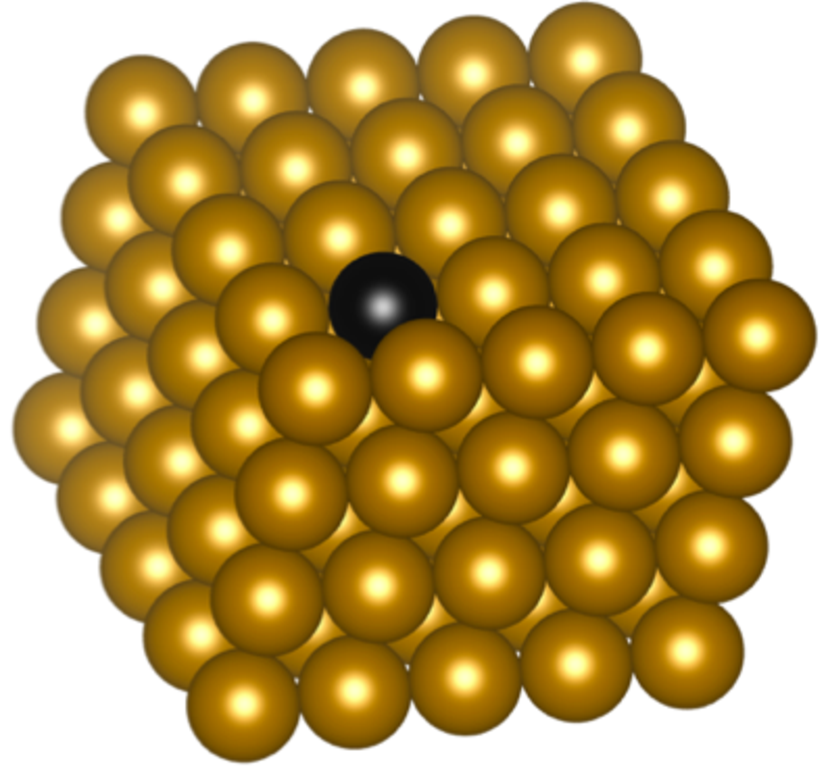
\includegraphics[width=0.25\linewidth]{Chap3/plots/Fig2a.pdf}}\label{Chap:Mg_H:fig:2a}
  \subfigure[]{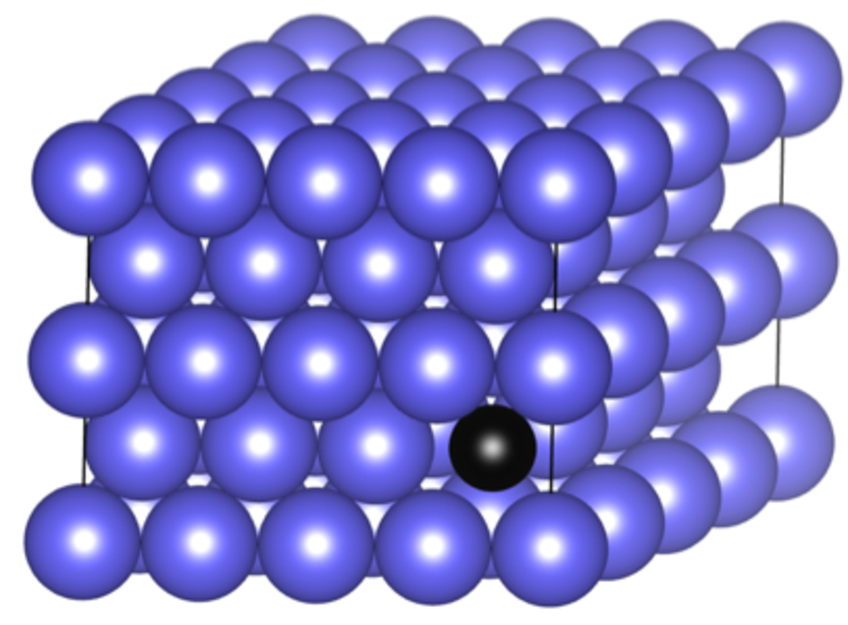
\includegraphics[width=0.25\linewidth]{Chap3/plots/Fig2b.pdf}}\label{Chap:Mg_H:fig:2b}\\
  \subfigure[]{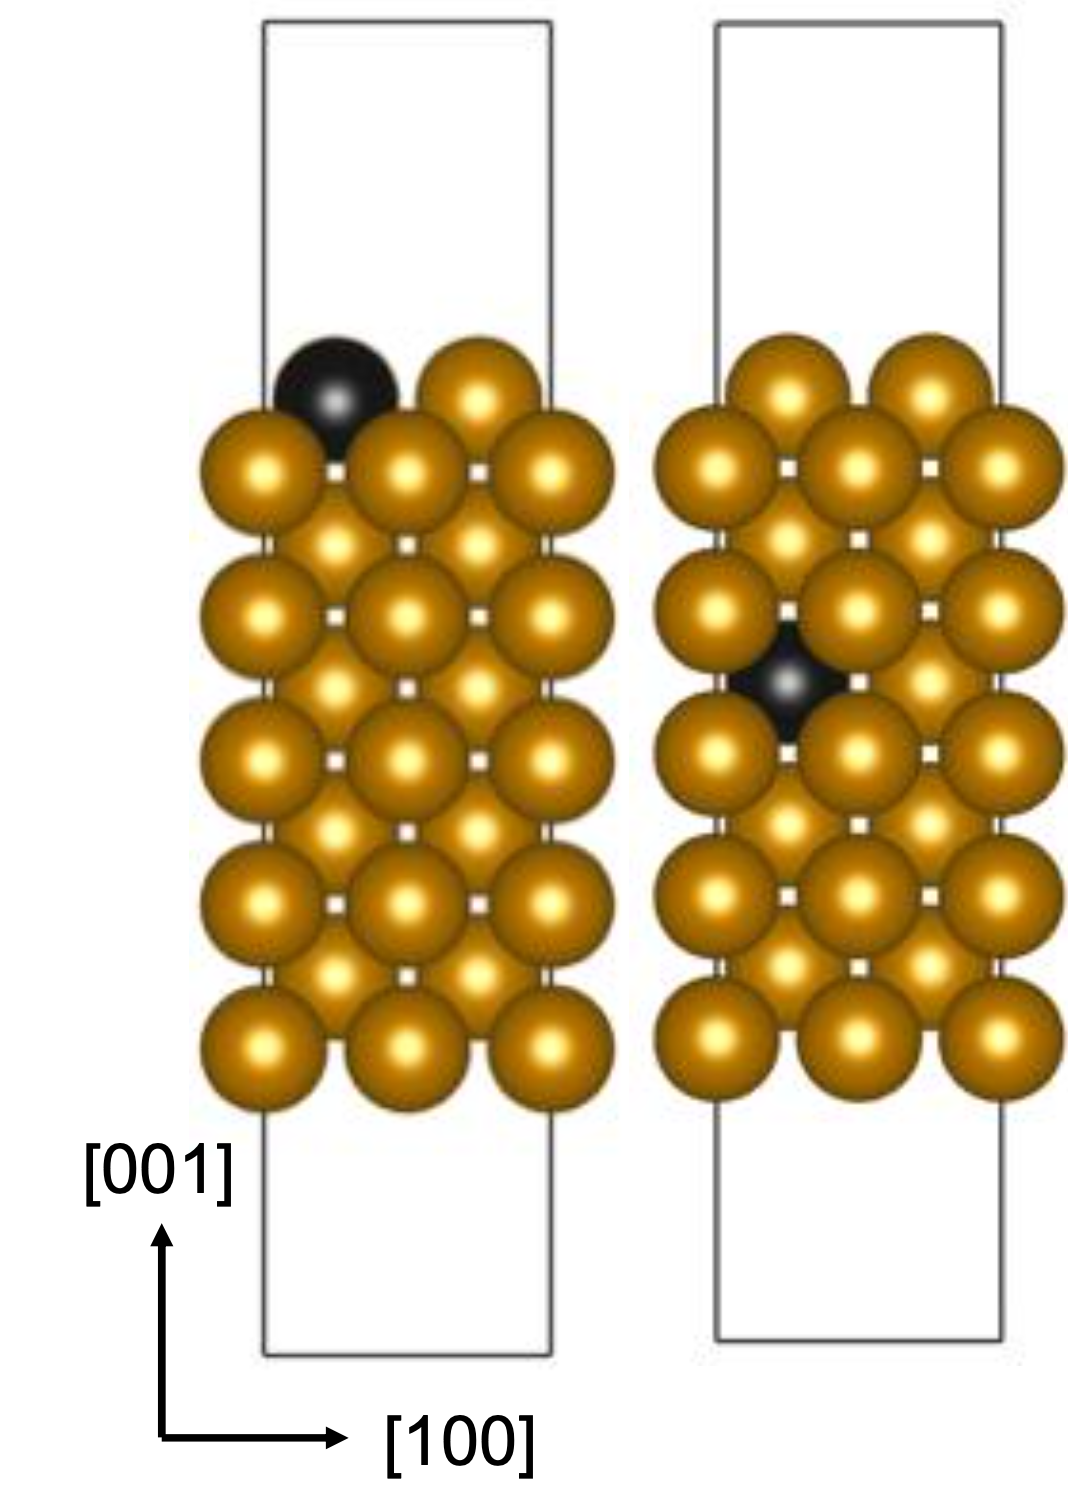
\includegraphics[width=0.25\linewidth]{Chap3/plots/Fig2c.png}}\label{Chap:Mg_H:fig:2c}
  \subfigure[]{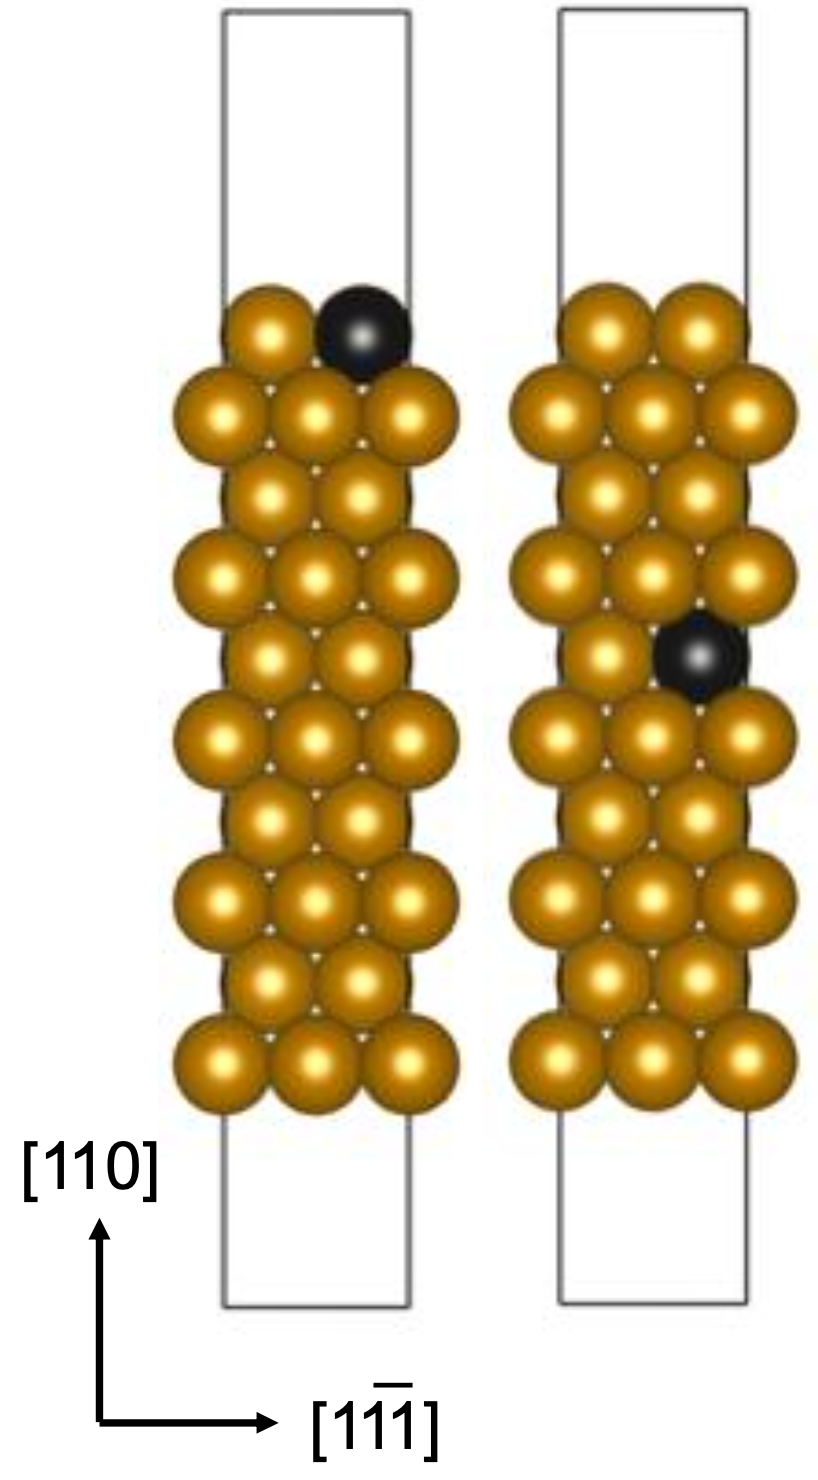
\includegraphics[width=0.25\linewidth]{Chap3/plots/Fig2d.png}}\label{Chap:Mg_H:fig:2d}
\caption[Perspective and side views of a generic alloying element in the simulation]{(a) and (b): Perspective view of a generic alloying element (black) in (a) bulk Fe (gold) and (b) bulk Mg (blue) lattice. (c)/(d): Side views of a generic alloying element (black) positioning in (2x2) Fe (100) (c) /Fe (110) (d) surface slab (the left sub-figure) at a substitutional site in the top surface layer and (the right sub-figure) at a substitutional site inside bulk Fe ($5^{th}$ layers from the top surface).}
  \label{Chap:Mg_H:fig2}
\end{figure}
\endgroup

Experimentalists have identified Arsenic (As) and Germanium (Ge) as Mg corrosion inhibitors. These are thought to exert a form of “kinetic control” over Mg corrosion, which is somewhat surprising from the standpoint that most elements tend to increase Mg corrosion rates \cite{liu2016controlling}. Eaves et al. \cite{eaves2012inhibition} were among the first to report that As is an effective corrosion inhibitor for commercially pure Mg with 280 ppm Fe in aqueous NaCl electrolyte. A subsequent report by Birbilis et al. \cite{birbilis2014evidence} proposed that As effectively ``poisons'' Mg corrosion by acting as a barrier for hydrogen intermediate (H*) recombination on surfaces of Fe particles (i.e. the cathode sites) thereby disrupting the formation of $\text{H}_2$(g) and, consequently, the \ac{HER} reaction. Noting that As is carcinogenic to humans, Liu et al. \cite{liu2016controlling,liu2018simultaneously} explored Ge and Ge-Zn metallurgically alloyed with pure Mg and found that Ge also interferes with cathode reactions. Other investigations have focused on adding rare earth elements to Mg \cite{birbilis2009corrosion,liu2009effect,shi2013corrosion}. New Mg-Li and Mg-Sn alloys were recently reported in which protective surface films form that prevent corrosion \cite{xu2015high,cain2019corrosion}. While these studies have pointed to an effect of a few elemental additives on Mg corrosion, the experimental literature has not, to our knowledge, provided a more expansive study of Mg corrosion inhibiting elements, and it is essentially silent regarding the role of electronic structure and chemical bonding at surfaces of Fe particles especially with regards to possible disruption of the \ac{HER}.

In this chapter, we use a high-throughput computational procedure based on \ac{DFT} to search for potential Mg corrosion inhibiting elements. We first search for other elements that can effectively slow down/disrupt the \ac{HER} by computing H adsorption energies on clean Fe surfaces with different alloying elements. Under realistic electrochemical conditions, there are other atoms/molecules and reaction intermediates, such as O atoms, OH groups and water molecules that affect the overall \ac{HER} rate, and multiscale simulations would be required to output accurate electrochemical rates \cite{qi2012adsorbate}. Alternatively, clean metallic surfaces have been widely used as effective model systems to quantitatively evaluate the relative changes of surface reaction rates, including those related to the \ac{HER} on pure and doped Mg surfaces \cite{williams2016modeling,pozzo2009hydrogen}. In general, the H adsorption energy on clean metallic surfaces has been proven to be an effective ``descriptor'' of \ac{HER} rates on these surfaces \cite{greeley2006computational}.

\newpage
\begingroup
\begin{figure}[!ht]
  \centering
  \subfigure[]{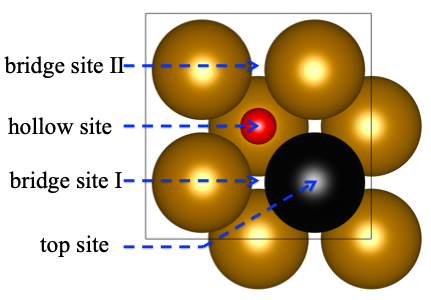
\includegraphics[width=0.5\linewidth]{Chap3/plots/Fig3a.png}}\label{Chap:Mg_H:fig:3a}
  \subfigure[]{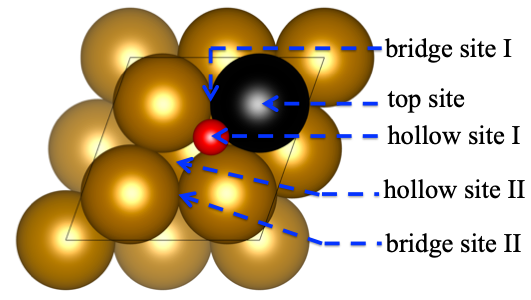
\includegraphics[width=0.55\linewidth]{Chap3/plots/Fig3b.png}}\label{Chap:Mg_H:fig:3b}
\caption[Top-down views of Fe surfaces with substitutional alloying elements and adsorbed H atoms]{Top-down views of Fe (gold) surfaces with substitutional alloying (black) elements and adsorbed H (red) atoms. (a) The (2x2) Fe (100) slab with a generic alloying element substituting a Fe atom in the top surface layer and an adsorbed H atom at the hollow site. (a) The (2x2) Fe (110) slab with a generic alloying element substituting a Fe atom in the top surface layer and an adsorbed H atom at the hollow site I. The concentration of the adsorbed H and the substitutional alloying atom is $\frac{1}{4}$ \ac{ML} for both Fe (100) and Fe (110).}
  \label{Chap:Mg_H:fig3}
\end{figure}
\endgroup
\section{Criteria to determine candidate elements to inhibit Mg corrosion}
\label{chap:Mg_H:sec:criteria}

The following three criteria were applied to determine if an alloying element could potentially inhibit Mg corrosion by slowing down the \ac{HER} as the cathodic reaction on surfaces of Fe-rich second-phase particles. (1) The alloying element must show a thermodynamic preference for bulk Fe over bulk Mg. (2) The alloying element must be thermodynamically more stable on Fe surfaces than in bulk Fe. (3) The adsorption energies of a lone H atom on Fe surfaces with an alloying element in their topmost layers should be significantly reduced (or enhanced) relative to the adsorption energies of a lone H atom on pure Fe surfaces, suggesting possible interference with $\text{H}_2$(g) formation and a consequent decrease in the \ac{HER} rate. Therefore, criterion 3 requires that a potential candidate significantly increase or reduce H adsorption strength on Fe particle surfaces.


The second and third criteria require the investigation of specific Fe surfaces. The Wulff plot shows (100) and (110) surfaces of a \ac{BCC} Fe single crystal are the two-major low-index surfaces at equilibrium conditions; (100) and (110) occupy more than $\text{50}\%$ of the \ac{BCC} Fe surface area and have the lowest energies\cite{tran2016surface}. Other high-index surfaces are also combinations of these two surfaces with steps. Therefore, our high-throughput search was conducted on models constructed with either (100) or (110) surfaces of \ac{BCC} Fe.

\begingroup
\begin{figure}[!ht]
  \centering
  \subfigure{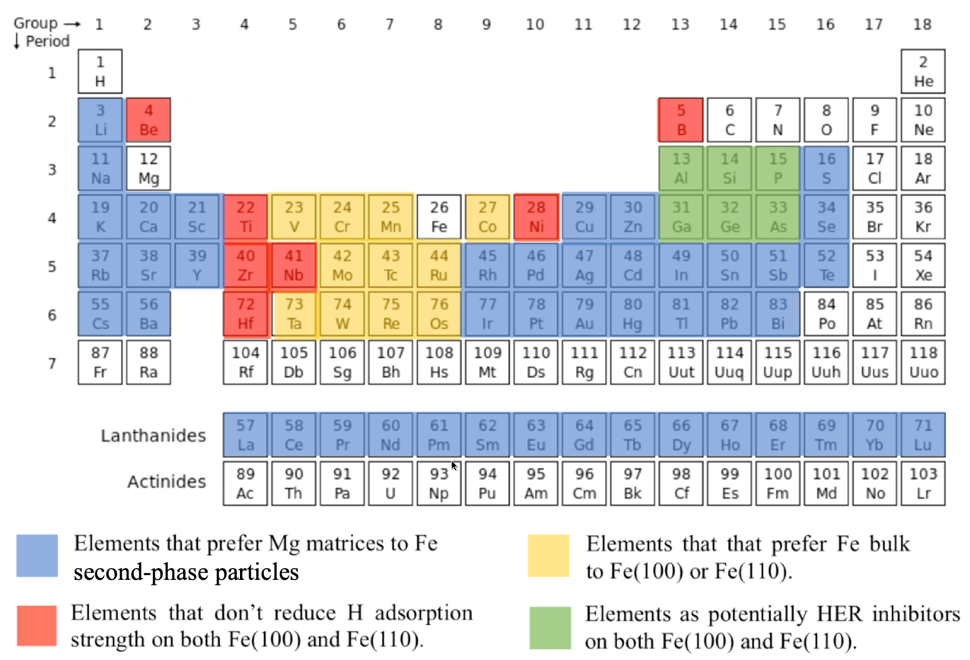
\includegraphics[width=1.0\linewidth]{Chap3/plots/Fig4.png}}
  \caption[Summary of the high-throughput search for alloying elements that can inhibit \ac{HER} on surfaces of Fe second-phase particles in Mg matrix.]{Summary of the high-throughput search for alloying elements that can inhibit \ac{HER} on surfaces of Fe second-phase particles in Mg matrix. All investigated alloying elements are labeled in colors (blue, yellow, red and green). Different colors describe the search results for the corresponding alloying elements as explained in the figure legends. (White periodic table from Wikimedia Commons)}
  \label{Chap:Mg_H:fig4}
\end{figure}
\endgroup

% \section{First-principles calculation methods and high-throughput search approach}
% \label{chap:Mg_H:sec:calculation}

The first criterion requires that a Mg corrosion-inhibiting element must have a thermodynamic preference for bulk Fe over bulk Mg. Hence, models aimed at examining bulk segregation energetics were constructed. To simulate bulk Fe, we constructed a 4$\times$4$\times$4(64 atoms) supercell (each primitive cell consists of 1 Fe atom). To simulate bulk Mg, we constructed a 4$\times$4$\times$2 supercell (64 atoms) with each primitive cell consisting of 2 Mg atoms. An element (e.g. As) was then placed at an Fe substitutional site in the bulk Fe supercell and at a Mg substitutional site in the Mg bulk supercell, as shown in Figs. 2(a) and 2(b), respectively.


To address the second criterion (an element must have a thermodynamic preference for Fe (100) and Fe (110) surfaces rather than for bulk Fe), four models aimed at examining Fe surface segregation energetics were constructed. Each consisted of 40 atoms in the Fe (100) and Fe (110) slabs with 10 layers of 2$\times$2 surface periodicity and a 12$\angstrom$ vacuum.  Two of the models contained an element placed at an Fe substitutional site in the top surface layers of Fe (100) and Fe (110) (i.e. where the \ac{HER} is expected to occur). These models are shown in Figs. 2(c) and 2(d), respectively. For the remaining two models, also shown in Figs. 2(c) and 2(d), an element (e.g. As) was placed at an Fe substitutional site five layers below the top surface.


\newpage
\begingroup
\begin{figure}[!ht]
  \centering
  \subfigure[]{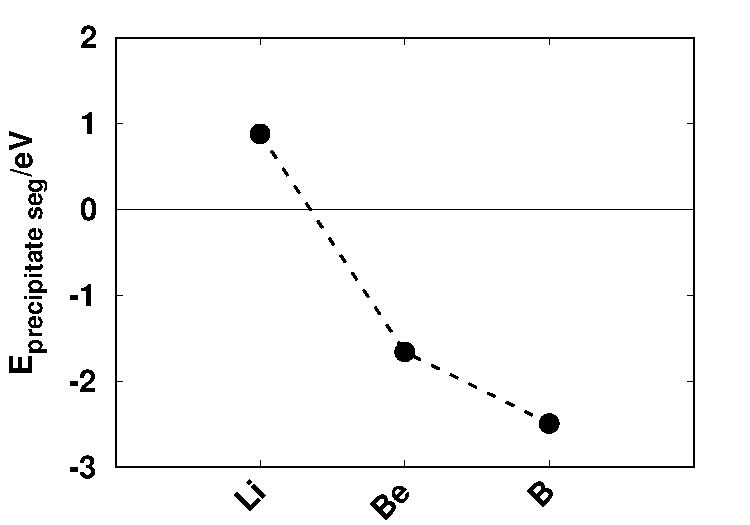
\includegraphics[width=0.46\linewidth]{Chap3/plots/Fig5a.pdf}}\label{Chap:Mg_H:fig:5a}
  \subfigure[]{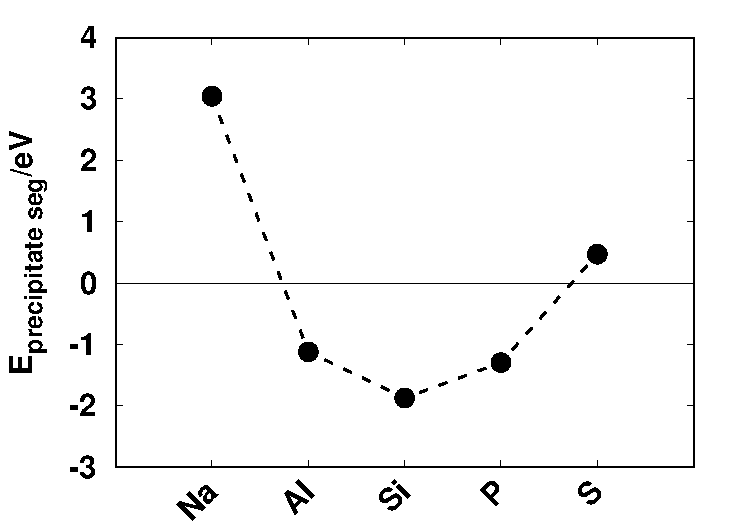
\includegraphics[width=0.46\linewidth]{Chap3/plots/Fig5b.pdf}}\label{Chap:Mg_H:fig:5b}
  \\
  \subfigure[]{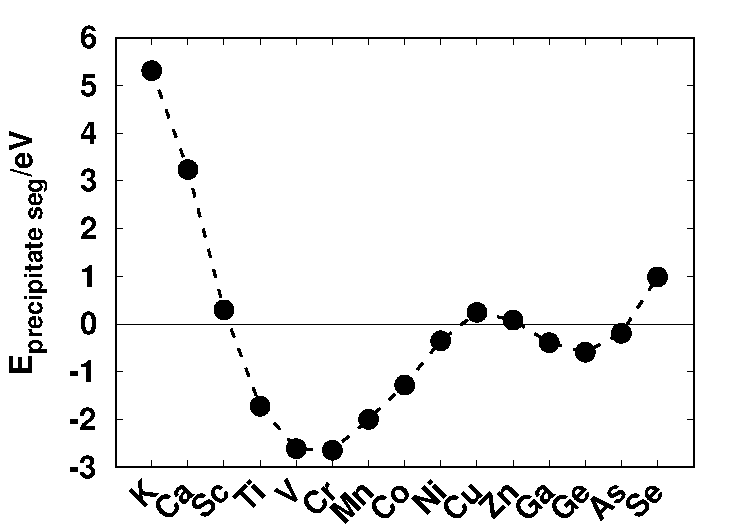
\includegraphics[width=0.46\linewidth]{Chap3/plots/Fig5c.pdf}}\label{Chap:Mg_H:fig:5c}
  \subfigure[]{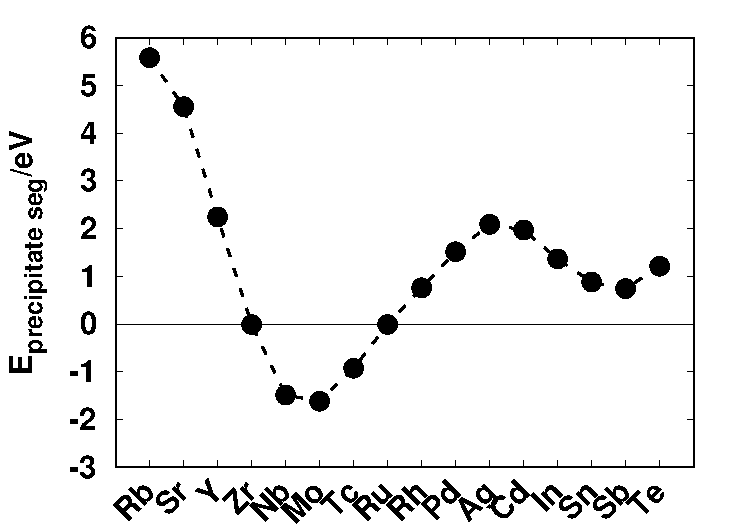
\includegraphics[width=0.46\linewidth]{Chap3/plots/Fig5d.pdf}}\label{Chap:Mg_H:fig:5d}
  \\
  \subfigure[]{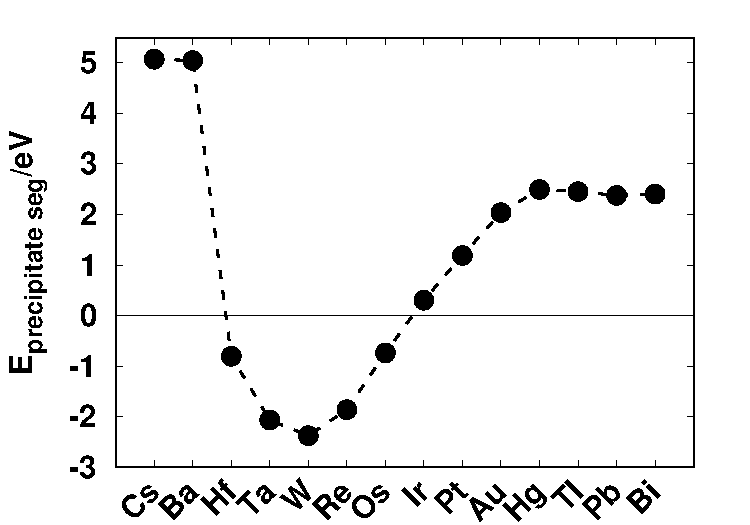
\includegraphics[width=0.46\linewidth]{Chap3/plots/Fig5e.pdf}}\label{Chap:Mg_H:fig:5e}
  \subfigure[]{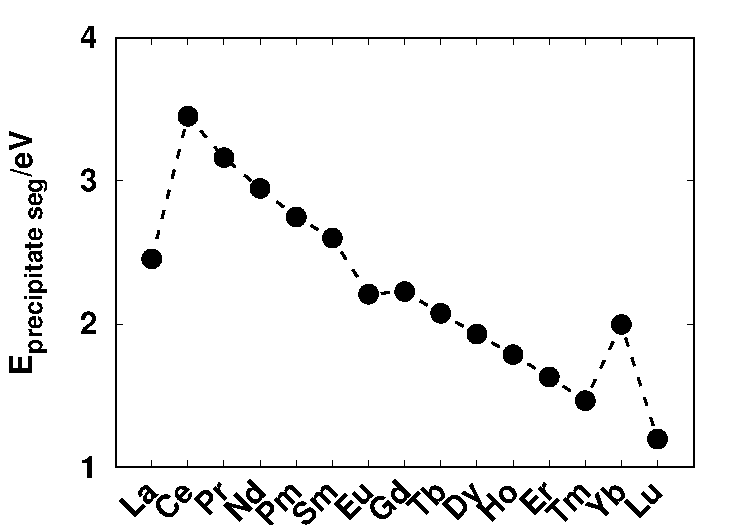
\includegraphics[width=0.46\linewidth]{Chap3/plots/Fig5f.pdf}}\label{Chap:Mg_H:fig:5f}
\caption[Segregation energies to bulk second-phase particles $E_{particle seg}$ defined in Equation \ref{Chap:Mg_H:eq:particle_seg} for the 68 potential alloying elements.]{Segregation energies to bulk second-phase particles $E_{particle seg}$ defined in Equation \ref{Chap:Mg_H:eq:particle_seg} for the 68 potential alloying elements. Preference for a \ac{BCC} Fe particle over the bulk \ac{HCP} Mg requires that an alloying element should have a significantly negative value of $E_{particle seg}$. (a)~(e): Elements in Row 2, 3, 4, 5 and 6 of the periodic table, respectively. (f) Lanthanide Elements. Elements with negative Eparticle seg are narrowed to 24: Be, B, Al, Si, P, Ti, V, Cr, Mn, Co, Ni, Ga, Ge, As, Zr, Nb, Mo, Tc, Ru, Hf, Ta, W, Re and Os.}
  \label{Chap:Mg_H:fig5}
\end{figure}
\endgroup

To address the third criterion that pertains to affecting H adsorption energies and possibly the HER rate, H adsorption energetics were investigated with both a single H atom adsorbed ($\frac{1}{4}$ \ac{ML}) at different sites on Fe (100) and Fe (110) with (2$\times$2) in-plane periodicity and an alloying element substituting a Fe atom in the top surface layer. On a (2$\times$2) Fe (100) with a substitutional alloying atom in the top layer, there are four possible H adsorption sites as shown in Figure \ref{Chap:Mg_H:fig3} (a): (1) a top site directly above 1 Fe atom or 1 alloying atom substituting for a Fe surface atom, (2) a bridge site I with 1 Fe atom and 1 alloying atom nearest neighbors (NNs), (3) a bridge site II with 2 Fe atoms as NNs, (4) a hollow site with 3 Fe atoms and 1 alloying atom NNs. On a (2$\times$2) Fe (110) with a substitutional alloying atom in the top layer, there are five H adsorption sites of interest as shown in Figure  \ref{Chap:Mg_H:fig3} (b): (1) a top site directly above 1 Fe atom or 1 alloying atom, (2) a bridge site I with 1 Fe atom and 1 alloying atom as NNs, (3) a bridge site II with 2 Fe atoms as NNs, (4) a hollow site I with 2 Fe atoms and 1 alloying atom as NNs, (5) a hollow site II with 3 Fe atoms as NNs.


The computational engine that provided the energetics used to evaluate the three criteria for each of the 68 candidate alloying elements was the implementation of \ac{DFT} in the \ac{VASP}. Each model was spin-polarized to account for \ac{BCC} Fe ferromagnetism. All-electron \ac{PAW} potentials were employed for the elemental constituents with the \ac{GGA} of \ac{PBE} for the exchange-correlation energy functional, $\mu_{xc}$, and the interpolation formula of Vosko et al.\cite{vosko1980accurate}. Using plane-wave cutoff energy of at 450.0 eV, the total energy for all models was converged to $10^{−7}$ eV/cell, and the force components on each atom were relaxed to less than $10^{−3}$ eV/Å. The reciprocal space of Fe (110), Fe (100) and bulk supercells were sampled with (16$\times$16$\times$1), (14$\times$14$\times$1), and (8$\times$8$\times$8) k-point grids, respectively. Each grid was generated using the Monkhorst-Pack scheme \cite{monkhorst1976special}. A 20$\angstrom$$\times$20$\angstrom$$\times$20$\angstrom$ supercell with a $\text{H}_2$ molecule in the middle was used for this calculation. The reciprocal space was sampled with a (1$\times$1$\times$1) Gamma centered k-points grid. Using plane-wave cutoff energy of at 450.0 eV, the total energy for all models was converged to $10^{−7}$ eV/cell.


Two successive structural optimizations (adapting basis vectors and computational grids to the cell parameters) were conducted on the bulk solids to ensure that the cell energies and structural parameters were fully converged. A \ac{VASP}-optimized lattice parameter of 2.83 $\angstrom$ for \ac{BCC} Fe was computed (the experimental room temperature value is 2.87 $\angstrom$\cite{kohlhaas1967temperature}) along with a 2.197 $\mu B/atom$ spin moment. Our computed spin moment is in good agreement with the 2.2 $\mu B/atom$ value from the \ac{DFT} study of Tiago et al.\cite{tiago2006evolution}. For \ac{HCP} Mg, the VASP-optimized lattice parameters are: a=3.19 $\angstrom$, c/a = 1.62 (the room temperature experimental values are: a=3.32 $\angstrom$, c/a = 1.62\cite{wrobel2012thermodynamic}). DFT calculations predict Fe (110) to have the lowest surface energy (2.40 $J/m^2$) and Fe (100) to have the second-lowest surface energy (2.45 $J/m^2$), in accord with previous DFT studies of Fe surfaces\cite{hung2002first}.  Experiments, however, identify (100) as having the lowest surface energy\cite{tyson1977surface}. Possible reasons for the disparity between DFT and experiments are provided by Hung et al.\cite{hung2002first}.

\newpage
\begingroup
\begin{figure}[!ht]
  \centering
  \subfigure[]{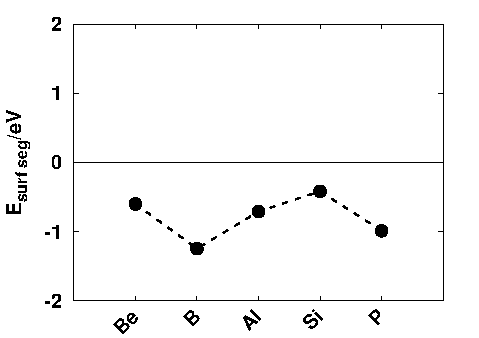
\includegraphics[width=0.49\linewidth]{Chap3/plots/Fig6a.pdf}}\label{Chap:Mg_H:fig:6a}
  \subfigure[]{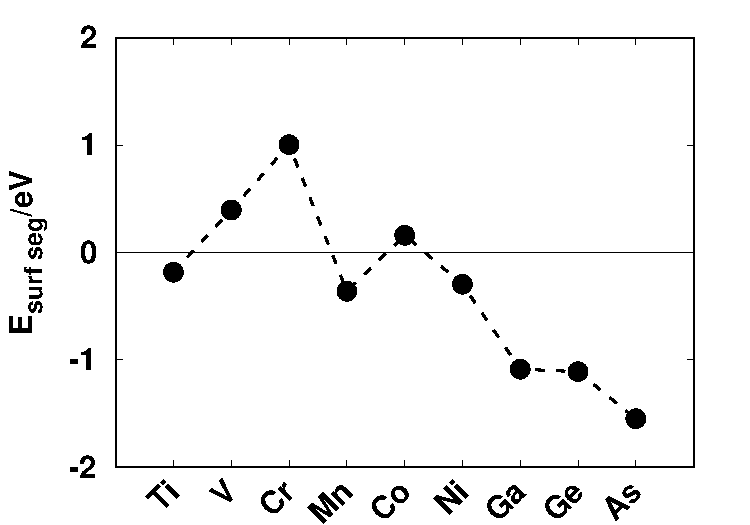
\includegraphics[width=0.49\linewidth]{Chap3/plots/Fig6b.pdf}}\label{Chap:Mg_H:fig:6b}
  \\
  \subfigure[]{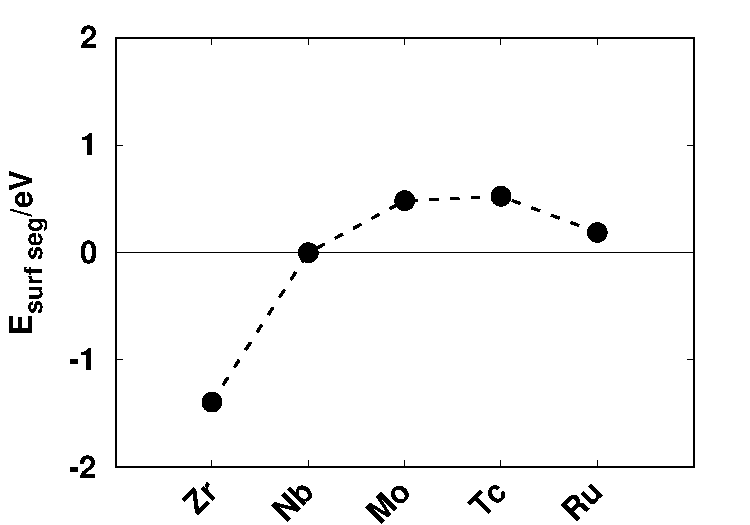
\includegraphics[width=0.49\linewidth]{Chap3/plots/Fig6c.pdf}}\label{Chap:Mg_H:fig:6c}
  \subfigure[]{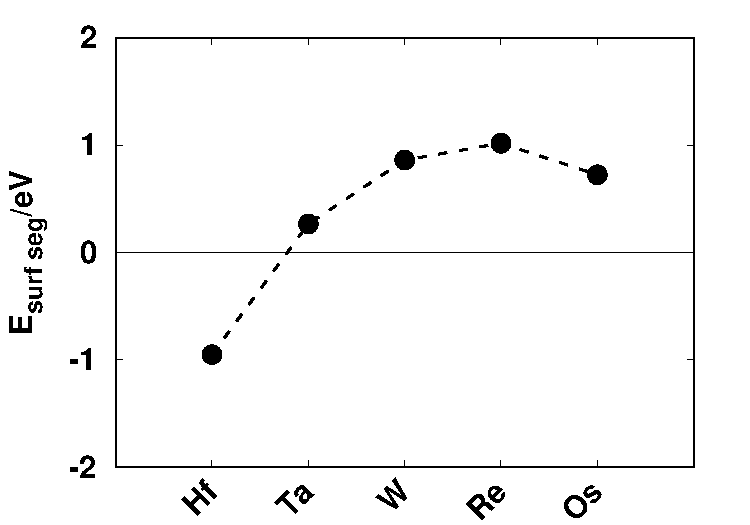
\includegraphics[width=0.49\linewidth]{Chap3/plots/Fig6d.pdf}}\label{Chap:Mg_H:fig:6d}
\caption[Segregation energies $E_{surf seg}$ defined in Equation \ref{Chap:Mg_H:eq:surf_seg} for Fe (100) of 24 alloying elements narrowed from the first screening round.]{Segregation energies $E_{surf seg}$ defined in Equation \ref{Chap:Mg_H:eq:surf_seg} for Fe (100) of 24 alloying elements narrowed from the first screening round. A qualified alloy candidate should have a strongly negative value of $E_{surf seg}$. (a): Elements in Row 2 and 3 of the periodic table. (b)~(d): Elements in Row of 4, 5 and 6 of the periodic table, respectively.}
  \label{Chap:Mg_H:fig6}
\end{figure}
\endgroup

Other than H adsorption energetics, there are two other criteria that are important as mentioned in Section 2.1: (1) an alloying element X should be more thermodynamically stable in bulk \ac{BCC} Fe instead of bulk \ac{HCP} Mg, (2) an alloying element X should segregate to an Fe surface rather than remaining in bulk Fe. Regarding the first criterion, we calculated the segregation energy to the second-phase particle, $E_{particle seg}$, via
\begin{align}
 E_{particle seg} = (\frac{63}{64}E_{Mg64} + E_{Fe63}X) - (E_{Mg63}X + \frac{63}{64}E_{Fe64})
 \label{Chap:Mg_H:eq:particle_seg}
\end{align}
where $E_{Mg64}$, $E_{Fe63X}$, $E_{Mg63X}$, and $E_{Fe64}$ are the total energies of 64-atom supercells for pure bulk HCP Mg, bulk \ac{BCC} Fe with 1 substitutional X atom (see Figure \ref{Chap:Mg_H:fig2} (a)), bulk HCP Mg with 1 substitutional X atom (see Figure \ref{Chap:Mg_H:fig2} (b)), and pure bulk \ac{BCC} Fe, respectively. A negative value of $E_{particle seg}$ for a given X means that it is energetically favorable for X to bind to bulk Fe instead of segregating to bulk Mg. The results show that a substitutional As atom has an energetic preference for bulk Fe over bulk Mg using the models shown in Figure \ref{Chap:Mg_H:fig2} (a) and \ref{Chap:Mg_H:fig2} (b), with a computed segregation energy of -0.19 eV.

\newpage
\begingroup
\begin{figure}[!ht]
  \centering
  \subfigure[]{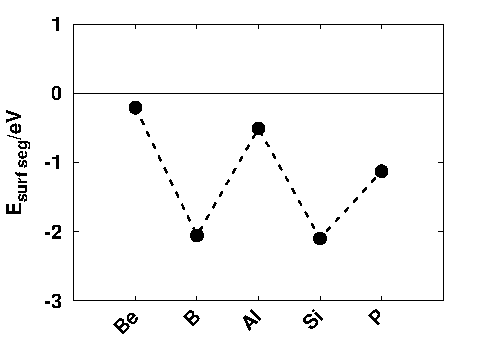
\includegraphics[width=0.49\linewidth]{Chap3/plots/Fig7a.pdf}}\label{Chap:Mg_H:fig:7a}
  \subfigure[]{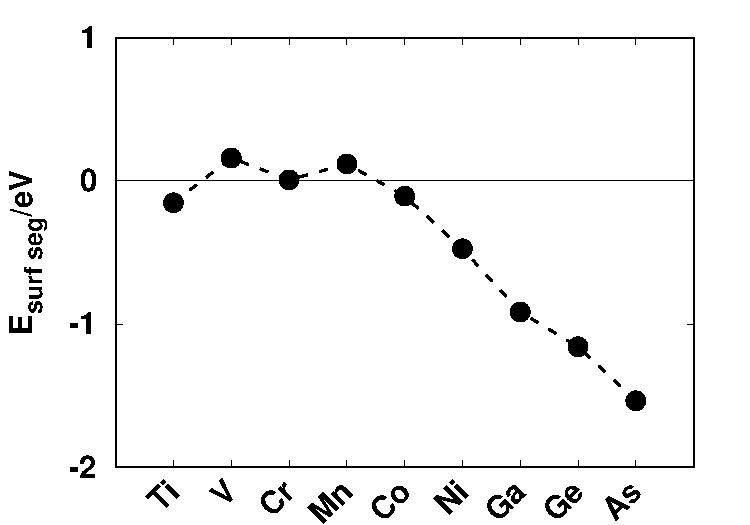
\includegraphics[width=0.49\linewidth]{Chap3/plots/Fig7b.pdf}}\label{Chap:Mg_H:fig:7b}
  \\
  \subfigure[]{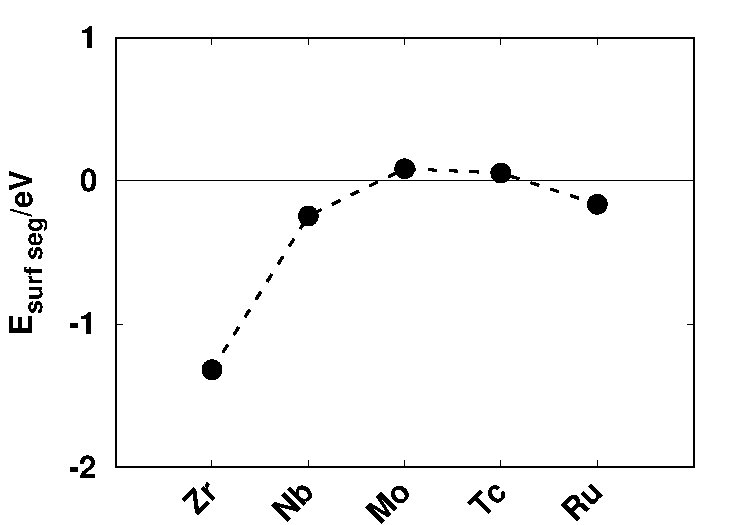
\includegraphics[width=0.49\linewidth]{Chap3/plots/Fig7c.pdf}}\label{Chap:Mg_H:fig:7c}
  \subfigure[]{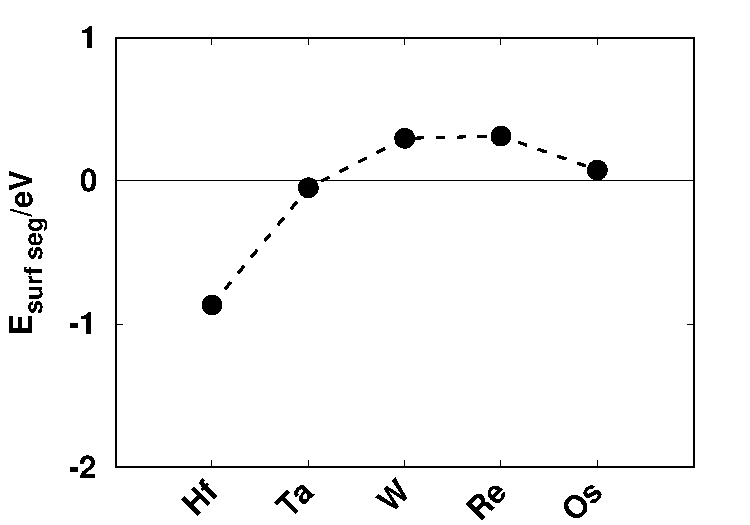
\includegraphics[width=0.49\linewidth]{Chap3/plots/Fig7d.pdf}}\label{Chap:Mg_H:fig:7d}
\caption[Segregation energies $E_{surf seg}$ defined in Equation \ref{Chap:Mg_H:eq:surf_seg} for Fe (110) of 24 alloying elements narrowed from the first screening round.]{Segregation energies $E_{surf seg}$ defined in Equation \ref{Chap:Mg_H:eq:surf_seg} for Fe (110) of 24 alloying elements narrowed from the first screening round. A qualified alloy candidate should have a strongly negative value of $E_{surf seg}$. (a): Elements in Row 2 and 3 of the periodic table. (b)~(d): Elements in Row of 4, 5 and 6 of the periodic table, respectively.}
  \label{Chap:Mg_H:fig7}
\end{figure}
\endgroup

Regarding the second criterion, we calculated the surface segregation energy of a substitutional alloying atom, $E_{surf seg}$, via:
\begin{align}
 E_{surf seg} = E_{surf} - E_{bulk}
 \label{Chap:Mg_H:eq:surf_seg}
\end{align}
where $E_{surf}$ and $E_{bulk}$ are the \ac{DFT}-computed energies of the corresponding surface slab with a substitutional alloying atom in the top surface layer (left figure in either Figure \ref{Chap:Mg_H:fig2} (c) or \ref{Chap:Mg_H:fig2} (d)) and the surface slab with a substitutional alloying atom inside the bulk (right figure in either Figure \ref{Chap:Mg_H:fig2} (c) or \ref{Chap:Mg_H:fig2} (d)), respectively). A negative $E_{surf seg}$ suggests that an alloying element will preferentially occupy an Fe site in the top surface layer instead of a site within bulk Fe. The results show that As prefers Fe (100) and Fe (110) instead of bulk Fe with computed segregation energies of -1.55 eV and -1.54 eV, respectively. Similar computations based on Equation \ref{Chap:Mg_H:eq:particle_seg} and \ref{Chap:Mg_H:eq:surf_seg} were conducted for the other 67 elements noted in Figure \ref{Chap:Mg_H:fig4} and detailed below.

The H adsorption energy, $E_{ad}^H$, was computed from
\begin{align}
 E_{ad}^{H} = E_{H/slab} - E_{slab} - \frac{1}{2}E_{H_2}(g)
 \label{Chap:Mg_H:eq:H_ads}
\end{align}

where $E_{H/slab}$ and $E_{slab}$ are the total energies of supercells of an Fe surface slab with/without adsorbed H atoms, respectively. $\text{H}_2$(g) is the energy of an isolated hydrogen gas molecule. Thus, the hydrogen adsorption strength is stronger with a more negative value of $E_{ad}^H$. The most stable H adsorption site on pure Fe (100) is the hollow site noted in Figure \ref{Chap:Mg_H:fig3} (a) with $E_{ad}^H$ = -0.38 eV. With an As atom substituting an Fe atom in the top surface layer of Fe (100), Table \ref{Chap:Mg_H:tab:H_ads} shows that $E_{ad}^H$ at the hollow site with an As NN in Figure \ref{Chap:Mg_H:fig3} (a) changes to -0.22 eV/atom. If H is initially placed at the top site above the substitutional As atom in the top layer of Fe (100), an unfavorable $E_{ad}^H$ = 0.67 eV is substantially different than the $E_{ad}^H$ = 0.20 eV for H at the top site of pure Fe (100) as listed in Table \ref{Chap:Mg_H:tab:H_ads}. If H is initially placed at bridge site I in Figure \ref{Chap:Mg_H:fig3} (a), it moves to the top site above the Fe NN during \ac{VASP} optimization. $E_{ad}^H$ at the bridge site II in Figure \ref{Chap:Mg_H:fig3} (a) is very similar to $E_{ad}^H$ at the bridge site of pure Fe (100) because there is no As as the NN.

\newpage
\begingroup
\begin{figure}[!ht]
  \centering
  \subfigure[]{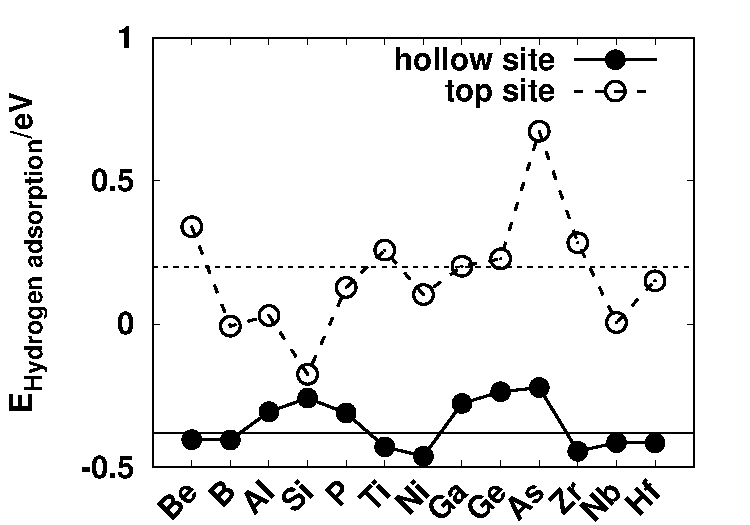
\includegraphics[width=0.6\linewidth]{Chap3/plots/Fig8a.pdf}}\label{Chap:Mg_H:fig:8a}
  \subfigure[]{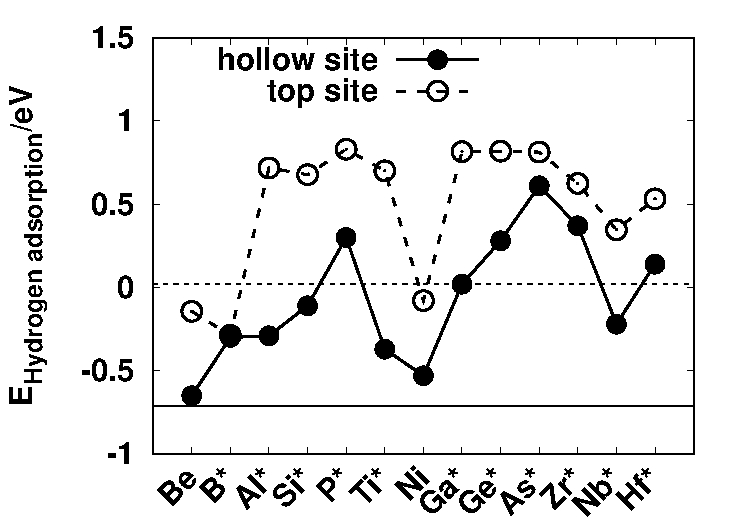
\includegraphics[width=0.6\linewidth]{Chap3/plots/Fig8b.pdf}}\label{Chap:Mg_H:fig:8b}
\caption[H adsorption energies $E_{ad}^H$ defined in Equation \ref{Chap:Mg_H:eq:H_ads} on Fe (100) and Fe (110) with the 13 alloying elements that pass the second screening round.]{H adsorption energies $E_{ad}^H$ defined in Equation \ref{Chap:Mg_H:eq:H_ads} on Fe (100) and Fe (110) with the 13 alloying elements that pass the second screening round. (a) H adsorption energies at the hollow site and the top site on Fe (100) with different alloying elements. Their surface geometry is shown in Figure \ref{Chap:Mg_H:fig3} (a). The horizontal solid and dash lines are the hydrogen adsorption energy at the hollow site and top site of pure Fe (100), respectively. (b) H adsorption energies at the hollow site I and the top site on Fe (110) with different alloying elements. Their surface geometry is shown in Figure \ref{Chap:Mg_H:fig3} (b). The horizontal solid and dash lines are the hydrogen adsorption energy at the hollow site I and top site on a pure Fe surface, respectively. H adsorption energies at the hollow site I on Fe (110) surfaces with B, Al, Si, P, Ti, Ga, Ge, As, Zr, Nb and Hf (marked with *) were computed by only allowing H and surface atoms to relax in the direction normal to the Fe (110).}
  \label{Chap:Mg_H:fig8}
\end{figure}
\endgroup
\section{High Throughput Screening Results}

We next examined the remaining 67 elements identified in Fig. \ref{Chap:Mg_H:fig4} (all elements with colors in the periodic table) with high-throughput DFT computations. Three successive rounds of calculations, each aimed at addressing one of the three criteria listed in Section 2.1, were conducted to narrow down the broader pool of elements highlighted in Fig. \ref{Chap:Mg_H:fig4}. In the first round, we examined Fe segregation energies to determine which of the remaining elements in Fig. \ref{Chap:Mg_H:fig4} prefers to segregate to bulk Fe rather than bulk Mg. This is the basis of the first criteria. In the second round, we determined which of those elements that passed the first round have favorable binding to Fe (100) and Fe (110) relative to bulk Fe. This is the basis of the second criteria. In the third and final round, we investigated which elements can either significantly weaken or strengthen H adsorption on Fe (110) and Fe (100).

For the first round, we calculated the second-phase particle segregation energy, $E_{particle seg}$,  of all alloying elements X (except As, which was previously addressed) denoted with colors in Fig. \ref{Chap:Mg_H:fig4} using Eq. \ref{Chap:Mg_H:eq:particle_seg}. As shown in Fig. \ref{Chap:Mg_H:fig5}, elements with negative $E_{particle seg}$ are narrowed to 24: Be, B (Fig \ref{Chap:Mg_H:fig:5a}), Al, Si, P (Fig. \ref{Chap:Mg_H:fig:5b}), Ti, V, Cr, Mn, Co, Ni, Ga, Ge, As (Fig. \ref{Chap:Mg_H:fig:5c}), Zr, Nb, Mo, Tc, Ru (Fig. \ref{Chap:Mg_H:fig:5d}), Hf, Ta, W, Re and Os (Fig. \ref{Chap:Mg_H:fig:5e}). No elements in the $7^{th}$ row or lanthanide series passed the first screening round (Fig. \ref{Chap:Mg_H:fig:5f}).

In the second round, we determined which of the 24 elements that passed the first screening round bind to Fe (100) and Fe (110) rather than to bulk Fe. The implication here is that potential slowing or even disruption of the HER can only occur if X preferentially binds to surfaces of Fe second-phase particles in an Mg alloy. We performed \ac{VASP} calculations with the remaining 24 elements adsorbed on Fe (100) and (110) using the models in Fig. \ref{Chap:Mg_H:fig:2c} and \ref{Chap:Mg_H:fig:2d}, where there is one atom of alloying element X in the top surface layer or the bulk layer of a (2x2) periodic unit cell. We calculated the surface segregation energy, $E_{surf seg}$, of all 24 elements using Eq. \ref{Chap:Mg_H:eq:surf_seg}. According to Fig. \ref{Chap:Mg_H:fig6}, only 13 elements from the pool of 24 from the second round were predicted to have favorable binding to Fe (100) ($E_{surf seg}$ < 0): Be, B, Al, Si, P (Fig. \ref{Chap:Mg_H:fig:6a}), Ti, Mn, Ni, Ga, Ge, As (Fig. \ref{Chap:Mg_H:fig:6b}), Zr (Fig. \ref{Chap:Mg_H:fig:6c}), and Hf (Fig. \ref{Chap:Mg_H:fig:6d}). Figure \ref{Chap:Mg_H:fig:6c} suggests that Nb has no preference for either Fe (100) or bulk Fe. We passed Nb on, nevertheless, to the third screening round. Similarly, Fig. 7 shows the same 13 candidates for Fe (110).  Hence, Be, B, Al, Si, P, Ti, Ni, Ga, Ge, As, Zr, Nb, and Hf are passed to the third and final screening round.

\begin{table}[ht]
\caption[Summary of H adsorption energies (eV/atom) defined at Equation \ref{Chap:Mg_H:eq:H_ads} at selected sites on (2$\times$2) Fe (100) and Fe (110) surface slabs without/with one substitutional atom from one of the 13 alloying elements that pass the second screening round.]{Summary of H adsorption energies (eV/atom) defined at Equation \ref{Chap:Mg_H:eq:H_ads} at selected sites on (2$\times$2) Fe (100) and Fe (110) surface slabs without/with one substitutional atom from one of the 13 alloying elements that pass the second screening round. H adsorption site is indicated at the top of each column and plotted in Figure 3(a) and 3(b). The ``stability'' at the top of the $5^{th}$ column means that H stays at the hollow site I on Fe (110) with substitutional alloying atoms as Figure 3(b) after the H and surface atoms are fully relaxed by \ac{VASP} optimization. Otherwise, the H adsorption energies at such hollow site I are calculated by only allowing the H and surface atoms to relax in the direction normal to the surface.}
\label{Chap:Mg_H:tab:H_ads}
\centering
\begin{tabular}{cccccc}
\\
\hline
\hline
        & \begin{tabular}[c]{@{}c@{}}(100) \\ top site\end{tabular} & \begin{tabular}[c]{@{}c@{}}(100) \\ hollow site\end{tabular} & \begin{tabular}[c]{@{}c@{}}(110)\\  top site\end{tabular} & \begin{tabular}[c]{@{}c@{}}(110) hollow \\ site I stability\end{tabular} & \begin{tabular}[c]{@{}c@{}}(110) hollow \\ site I\end{tabular} \\ \hline
Pure Fe & 0.2                                                       & -0.38                                                        & 0.02                                                      & Yes                                                                      & -0.71                                                          \\
Be      & 0.34                                                      & -0.4                                                         & -0.14                                                     & Yes                                                                      & -0.65                                                          \\
B       & -0.01                                                     & -0.4                                                         & -0.29                                                     & No                                                                       & -0.3                                                           \\
Al      & 0.03                                                      & -0.31                                                        & 0.72                                                      & No                                                                       & -0.29                                                          \\
Si      & -0.18                                                     & -0.26                                                        & 0.68                                                      & No                                                                       & -0.11                                                          \\
P       & 0.13                                                      & -0.31                                                        & 0.83                                                      & No                                                                       & 0.3                                                            \\
Ti      & 0.26                                                      & -0.43                                                        & 0.7                                                       & No                                                                       & -0.37                                                          \\
Ni      & 0.1                                                       & -0.46                                                        & -0.08                                                     & Yes                                                                      & -0.53                                                          \\
Ga      & 0.2                                                       & -0.28                                                        & 0.82                                                      & No                                                                       & 0.02                                                           \\
Ge      & 0.23                                                      & -0.24                                                        & 0.82                                                      & No                                                                       & 0.28                                                           \\
As      & 0.67                                                      & -0.22                                                        & 0.81                                                      & No                                                                       & 0.61                                                           \\
Zr      & 0.28                                                      & -0.44                                                        & 0.62                                                      & No                                                                       & 0.37                                                           \\
Nb      & 0.01                                                      & -0.41                                                        & 0.35                                                      & No                                                                       & -0.22                                                          \\
Hf      & 0.15                                                      & -0.42                                                        & 0.53                                                      & No                                                                       & 0.14                                                           \\ \hline\hline
\end{tabular}
\end{table}

In the third screening round, we investigated the H adsorption energies on both Fe (100) and Fe (110) with each of the 13 elements that passed the second screening round. Results are shown in Fig. 8 and Table \ref{Chap:Mg_H:tab:H_ads}. We used Eq. \ref{Chap:Mg_H:eq:H_ads} to calculate the H adsorption energies $E_{ad}^H$ on the two Fe surfaces with 1 alloying element X substituting a surface Fe atom as shown in Figs. \ref{Chap:Mg_H:fig:3a} and \ref{Chap:Mg_H:fig:3b}. Based upon our results for As, we limited the number of models for each Fe surface to two: H at the hollow site and at the top site of an alloying element X adsorbed on Fe (100) (Fig. \ref{Chap:Mg_H:fig:3a}), H at the hollow site I and at the top site of an alloying element X adsorbed on Fe (110) (Fig. \ref{Chap:Mg_H:fig:3b}). In the instance that an element X caused H to move from the hollow site I to the hollow site II on Fe (110), the same as the case for As, we only relaxed the H and the surface atoms along the direction normal to the surface to calculate $E_{ad}^H$. This decision was made after we fully relaxed all atoms on Fe (110) and determined which X causes H to move from its initial position. Whether to apply this restriction is summarized in Table \ref{Chap:Mg_H:tab:H_ads}, which uses the column of ``(110) hollow site I stability'' to indicate whether the H atom stays in the hollow site I (``Yes'' in that column) or moves to another site (``No'' in that column) after full relaxation.

Figs. \ref{Chap:Mg_H:fig8} shows H adsorption energies at hollow sites (the solid horizontal lines in both Figs. \ref{Chap:Mg_H:fig:8a} and \ref{Chap:Mg_H:fig:8b}) and top sites (the dashed horizontal lines in both Figs. \ref{Chap:Mg_H:fig:8a} and \ref{Chap:Mg_H:fig:8b}) on both pure Fe (100) and (110) surfaces, indicating that H prefers the hollow sites rather than the top sites. The same trend can be found for Fe surfaces with one of the 13 alloying element X as shown by the curved lines with open (for H at top sites) /solid (for H at hollow sites) circles in both Figs. \ref{Chap:Mg_H:fig:8a} and \ref{Chap:Mg_H:fig:8b}. The numerical values of the corresponding $E_{ad}^H$ for each case are listed in Table \ref{Chap:Mg_H:tab:H_ads}. Thus, the hydrogen adsorption energy at the hollow site was used as a numerical criterion to determine whether an alloying element can increase or reduce the hydrogen adsorption strength on Fe surfaces. For the Fe (100) surface, 6 of the 13 remaining alloying elements (As, Ge, Ga, P, Si, Al) resulted in a significant reduction of hydrogen adsorption strength on the hollow site, all of which have $E_{ad}^H$ values more positive than $E_{ad}^H$ for H at the hollow site on pure Fe (100) as shown in Fig. \ref{Chap:Mg_H:fig:8a}. The other 7 alloying elements (Be, B, Ti, Ni, Zr, Nb, and Hf) resulted in almost no changes or even slightly increased the hydrogen adsorption strength.

On Fe (110), the addition of an element X may cause H to move, as was observed for As. This had the net result of moving the H from hollow site I to hollow site II in Fig. \ref{Chap:Mg_H:fig:3b}. Interestingly, Be and Ni were the notable exceptions in the pool of the 13 alloying elements X investigated in the third screening round since H remained at hollow site I in the presence of either element as indicated by the ``Yes'' in the column of ``(110) hollow site I stability'' of Table \ref{Chap:Mg_H:tab:H_ads}. Comparison of the pure Fe (110) H adsorption energy of -0.71 eV at hollow site I with H adsorption energies at the same site on Fe (110) with one of the 13 X implies that each of these elements weakens H adsorption strength on an Fe surface. Moreover, this comparison leads to the following rank ordering of the 13 elements starting with As, which causes the greatest weakening of H adsorption strength, and ending with Be that weakens H adsorption strength the least: $\text{As} > \text{Zr} > \text{Ge} \approx \text{P} > \text{Hf} > \text{Ga} > \text{Si} > \text{Nb} > \text{Al} > \text{B} > \text{Ti} > \text{Ni} > \text{Be}$.

Comparison of the H adsorption energies between the (100) hollow site and (110) hollow site identifies six elements that significantly weaken or destabilize H adsorption on both Fe (100) and Fe (110) are: Al, Si, P, Ga, Ge, As. The inference here is that they will reduce \ac{HER} rates on both Fe surfaces by slowing the Volmer reaction in Eq. \ref{Chap:Mg_H:eq:Tafel}. Transition metal elements (Ti, Ni, Zr, Nb and Hf) and B can have opposite effects on hydrogen adsorption strengths on Fe (100) and Fe (110) surfaces, and hence changes to the \ac{HER} rate are likely to be quite small. Specifically, changes in hydrogen adsorption energies on Fe (100) with these transition metal elements are relatively minor, which are confirmed by further studies of Fe (100) with higher surface concentrations of substitutional alloying atoms in Sec. 4. Hence, these surfaces can still behave as active cathode sites with a fast \ac{HER} rate, resulting in their elimination from the candidate list of potential corrosion inhibitors. Beryllium has the most favorable H adsorption energies at both the Fe (110) hollow site I (-0.65 eV/atom) and the Fe (100) hollow site (-0.40 eV/atom) relative to corresponding H adsorption energies on the pure Fe surfaces (-0.71 eV atom for the Fe (110) hollow site I and -0.38 eV/atom at the Fe (100) hollow site), resulting in its elimination from the list.

Since all of the H adsorption energies on hollow sites of the alloyed Fe (100) (Fig. \ref{Chap:Mg_H:fig:3a}) are obtained based on VASP relaxations with no ancillary restrictions, we expect that these adsorption energies can be used to rank the order the final six elements (Al, Si, P, Ga, Ge, As) based upon reduction and/or destabilization of H adsorption to the Fe surfaces. According to the results in Table \ref{Chap:Mg_H:tab:H_ads}, these H adsorption energies suggest the following rank ordering by reduction of H adsorption strengths, and consequently, HER rates as: $\text{As} > \text{Ge} > \text{Si} > \text{Ga} > \text{P} \approx \text{Al}$. These p-block elements, which are highlighted in green in Fig. \ref{Chap:Mg_H:fig4}, are the final group of corrosion-inhibiting elements that resulted from the application of the three criteria discussed above in our high-throughput computations. Note that the high-throughput computations call out As and Ge as potentially the best corrosion inhibiting elements using the idealized models in Figs. \ref{Chap:Mg_H:fig2} and \ref{Chap:Mg_H:fig3}. 

This result is in qualitative accord with experiments \cite{liu2016controlling,birbilis2014evidence}. A recent experimental study shows that microalloying additions of Ge, Sb, Pb, Sn and Bi (group 14 and 15 elements) can reduce the cathodic kinetics upon Mg, and Mg-Ge alloys were demonstrated to have the highest corrosion resistance among them \cite{liu2018simultaneously}. Another experimental study on corrosion behavior of biodegradable Mg–X (X = Sn, Ga, In) alloys shows a low amount ($<$ 1 wt$\%$) of Ga is the most effective among these three elements to improve the corrosion resistance of Mg alloys \cite{kubasek2013structure}. We didn't consider the effects of In, Sn, Sb, Pb or Bi in our studies because our \ac{VASP} calculations suggest that these four elements prefer to stay in Mg matrix instead of Fe particles (Fig. \ref{Chap:Mg_H:fig4} and \ref{Chap:Mg_H:fig5}). In reality, even Sn, Sb, Pb and Bi may prefer to stay on the surfaces of Fe-rich particles relative to the Mg matrix due to surface segregation, and hence it possible that they reduce the cathodic kinetics to some extent.

\newpage
\begingroup
\begin{figure}[!ht]
  \centering
  \subfigure[]{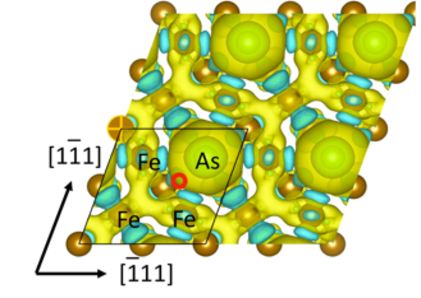
\includegraphics[width=0.45\linewidth]{Chap3/plots/Fig9a.pdf}}\label{Chap:Mg_H:fig:9a}
  \subfigure[]{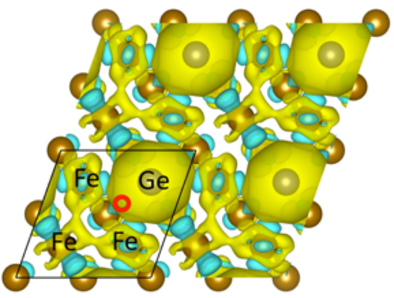
\includegraphics[width=0.45\linewidth]{Chap3/plots/Fig9b.pdf}}\label{Chap:Mg_H:fig:9b}
  \\
  \subfigure[]{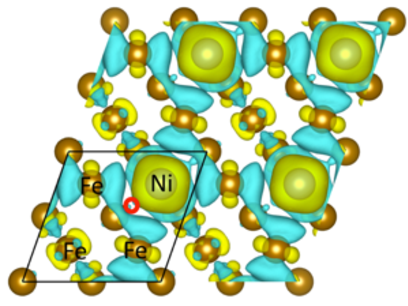
\includegraphics[width=0.45\linewidth]{Chap3/plots/Fig9c.pdf}}\label{Chap:Mg_H:fig:9c}
  \subfigure[]{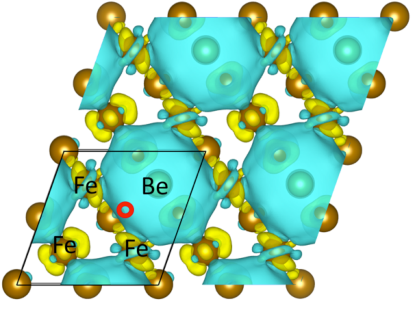
\includegraphics[width=0.45\linewidth]{Chap3/plots/Fig9d.pdf}}\label{Chap:Mg_H:fig:9d}  
\caption[Top-down views of isosurfaces of electron density difference for (2x2) Fe (110) with one substitutional alloying atom in top surface layer]{Top-down views of isosurfaces of electron density difference ($\Delta \rho$ defined in Eq. \ref{Chap:Mg_H:eq:chargediff}) for (2x2) Fe (110) with one substitutional alloying atom in top surface layer. Surface Fe and alloy element X (X as As, Ge. Ni and Be in (a), (b), (c) and (d), respectively) are denoted. The open red circle is located at a hollow site I (Fig. \ref{Chap:Mg_H:fig:3b}) for hydrogen adsorption. The black box indicates the periodicity of a (2x2) Fe (110). The yellowish isosurface is $1.5x10^{-3}\frac{e}{bohr^3}$ corresponding to positive $\Delta \rho$ or electron accumulation after the substitutional alloying. The blue isosurface is $-1.5x10^{-3}\frac{e}{bohr^3}$ corresponding to negative $\Delta \rho$ or electron depletion after the substitutional alloying.}
  \label{Chap:Mg_H:fig9}
\end{figure}
\endgroup






\section{Electronic Mechanism of Mg Corrosion Inhibition}

In general, chemisorption on a transition metal surface is determined by two factors: a potential attractive energy term ($E_{attractive}$) related to the d-band center location relative to the Fermi level (i.e. so-called d-band center model), and a repulsive energy term ($E_{repulsive}$) related to the orbital overlap between the adsorbate orbital and the orbitals of other surface atoms (so-called Pauli repulsion) \cite{hammer1995electronic,hammer1995gold}:
\begin{align}
 %(9)
E_{chem adsorption} \sim E_{attractive} + E_{repulsive}
\label{Chap:Mg_H:eq:electronic}
\end{align}

We found that the effect of each of the 6 p-block elements identified as Mg corrosion inhibitors in Section 3c is negligible on the d-band center of Fe surface atoms. This was confirmed by computing and examining electronic density-of-states (Section S1 of the Supplementary Materials). Specifically, when one Fe atom in the top surface layer of (2x2) Fe (100) or (110) was substituted by an alloying atom from one of 6 p-block elements, the change of d-band center for all atoms in the top surface layer was always less than 0.2 eV. According to previous DFT studies of a series of transition metals, a change of $\sim$1 eV in the d-band center of their surface atoms results in a change of $\sim$0.5 eV in H adsorption energy \cite{greeley2006computational}. Thus, it is not expected that such small changes in the d-band center for an Fe surface with p-block substitutional elements reported here can induce significant variations of hydrogen adsorption strengths.

\begingroup
\begin{figure}[!ht]
  \centering
  \subfigure[]{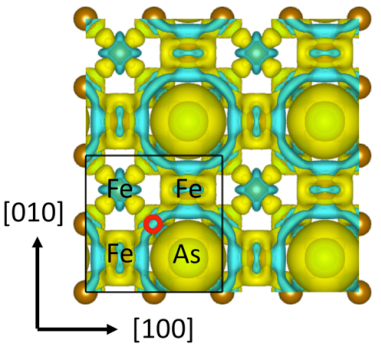
\includegraphics[width=0.45\linewidth]{Chap3/plots/Fig10a.pdf}}\label{Chap:Mg_H:fig:10a}
  \subfigure[]{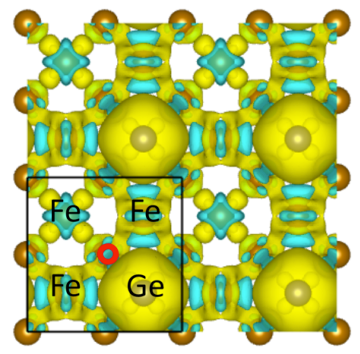
\includegraphics[width=0.45\linewidth]{Chap3/plots/Fig10b.pdf}}\label{Chap:Mg_H:fig:10b}
  \\
  \subfigure[]{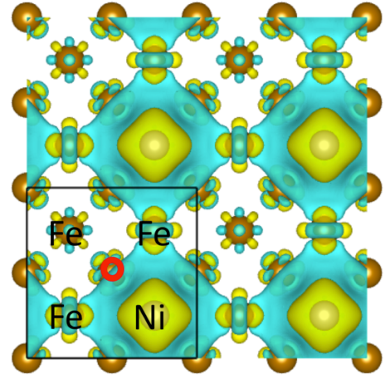
\includegraphics[width=0.45\linewidth]{Chap3/plots/Fig10c.pdf}}\label{Chap:Mg_H:fig:10c}
  \subfigure[]{\includegraphics[width=0.45\linewidth]{Chap3/plots/Fig10d.pdf}}\label{Chap:Mg_H:fig:10d}  
\caption[Top-down views of isosurfaces of electron density difference for (2x2) Fe (100) with one substitutional alloying atom in top surface layer]{Top-down views of isosurfaces of electron density difference ($\Delta \rho$ defined in Eq. \ref{Chap:Mg_H:eq:chargediff}) for (2x2) Fe (100) with one substitutional alloying atom in top surface layer. Surface Fe and alloy element X (X as As, Ge. Ni and Be in (a), (b), (c) and (d), respectively) are denoted. The open red circle is located at a hollow site I (Fig. \ref{Chap:Mg_H:fig:3b}) for hydrogen adsorption. The black box indicates the periodicity of a (2x2) Fe (100). The yellowish isosurface is $1.0x10^{-3}\frac{e}{bohr^3}$ corresponding to positive $\Delta \rho$ or electron accumulation after the substitutional alloying. The blue isosurface is $-1.0x10^{-3}\frac{e}{bohr^3}$ corresponding to negative $\Delta \rho$ or electron depletion after the substitutional alloying.}
  \label{Chap:Mg_H:fig10}
\end{figure}
\endgroup

We next examined surface charge redistribution by computing and displaying the difference, $\Delta \rho$, between the electron density of a pure (2x2) Fe (100)/(110) surface, $\rho_{Fe}$, and the electron density of the same surface unit cell with a substitutional X atom in the top surface layer, $\rho_{Fe+X}$, via
\begin{align}
 %(10)
\Delta \rho = \rho_{Fe+ X} - \rho_{Fe}
\label{Chap:Mg_H:eq:chargediff}
\end{align}
Results are shown in Figs. \ref{Chap:Mg_H:fig9} and \ref{Chap:Mg_H:fig10} for Fe (110) and Fe (100), respectively. Yellowish contours denote positive $\Delta \rho$ or regions of electron accumulation in the surface layer, while blue contours denote negative $\Delta \rho$ or electron depletion in the surface layer. Referring to Fig. \ref{Chap:Mg_H:fig:9a}, the yellowish contours surrounding the adsorbed As denote electron concentration in a shape resembling an s orbital with p-character. Fig. \ref{Chap:Mg_H:fig:9a} also shows a network of electron accumulation that encircles the As atom and flows through Fe surface atoms. This is somewhat counter-intuitive since As has five valence electrons, which is less than the eight in Fe. This electron accumulation around the As atom suggests the enhancement of both the spatial extent and electron density of the s/p orbital for the As atom compared with the pure Fe surface. When a H atom is absorbed at the hollow site near the As atom, indicated by the red circle in Fig. \ref{Chap:Mg_H:fig:9a}, the electrons from the adsorbed H atom and those from the substitutional As atom should overlap, and quantum mechanics requires that they must be orthogonal to each other. This drives up the energy and leads to so-called Pauli repulsion as described by $E_{repulsive}$ in Eq. \ref{Chap:Mg_H:eq:electronic}. Therefore, the s/p orbital for an As atom adsorbed on Fe (110) results in larger Pauli repulsion of the nearby H atom, making the H adsorption energy weaker relative to adsorption on a pure Fe surface. 

Similar effects were also predicted for adsorbed Ge on Fe (110), as shown in Fig. \ref{Chap:Mg_H:fig:9b}, as well as Al, Si, Ga, and P ($\Delta \rho$ contours not shown). Alternatively, the electron distribution is depleted around the adsorbed Ni atom in Fig. \ref{Chap:Mg_H:fig:9c} (relative to As in Fig. \ref{Chap:Mg_H:fig:9a}) and even more so around the adsorbed Be atom in Fig. \ref{Chap:Mg_H:fig:9d}. This is consistent with the observation from our high-throughput computations that neither Ni nor Be repels an H adsorbate on Fe surfaces, and the H adsorption energy in both cases is close to that of pure Fe (110). Observations for alloying elements on Fe (110) also apply to Fe (100) as shown in Fig. \ref{Chap:Mg_H:fig:10a} for As and Fig. \ref{Chap:Mg_H:fig:10b} for Ge (as well as Al, whose $\Delta \rho$ contours not shown). All of these elements have electron accumulation that resembles that for As on Fe (110) in Fig. \ref{Chap:Mg_H:fig:9a}, and their corresponding H adsorption energies notably change from -0.4 eV/atom to $\sim$ -0.2 eV/atom. Alternatively, Fig. \ref{Chap:Mg_H:fig:10c} shows that Ni has only a small local electron accumulation in Fe (100) while electron density is severely depleted around Be in Fig. \ref{Chap:Mg_H:fig:10d}. This is consistent with the conclusion from our high-throughput computations that H adsorption in the presence of Be and Ni on Fe (100) is not weakened.

\begingroup
\begin{figure}[!ht]
  \centering
  \subfigure[]{\includegraphics[width=0.45\linewidth]{Chap3/plots/Fig11a.pdf}}\label{Chap:Mg_H:fig:11a}
  \subfigure[]{\includegraphics[width=0.45\linewidth]{Chap3/plots/Fig11b.pdf}}\label{Chap:Mg_H:fig:11b}
  \\
  \subfigure[]{\includegraphics[width=0.45\linewidth]{Chap3/plots/Fig11c.pdf}}\label{Chap:Mg_H:fig:11c}
  \subfigure[]{\includegraphics[width=0.45\linewidth]{Chap3/plots/Fig11d.pdf}}\label{Chap:Mg_H:fig:11d}  
\caption[Effects of 6 p-block elements on higher surface alloying coverage]{(a) and (b): two different configurations ((a) as “config 1” and (b) as “config 2”)) for (2x2) Fe (100) with two atoms of a generic alloying element substituting two Fe atoms in the top surface layer. (c) Segregation energies $E_{surf seg}$ defined in Eq. (7) for the second substitutional alloying atom in (2x2) Fe (100) with two substitutional atoms in different final configurations ((a) and (b)). (d) H adsorption energies $E_{ad}^H$ defined in Eq. (8) on (2x2) Fe (100) with two substitutional alloying atoms in the top surface layer as “config 2” shown in (b).}
  \label{Chap:Mg_H:fig11}
\end{figure}
\endgroup
\section{Sensitivity Analysis for H Adsorption Energy on Surface Alloying Coverage}

All of the above evaluations are based on the three criteria in Section 2.1 with relatively simple but well-defined Fe surface structures with alloying elements. However, the quantitative predictions of alloying effects to Mg corrosion resistance require the accurate descriptions of surface and bulk structures of Fe-rich particles. As shown in Figure \ref{Chap:Mg_H:fig1} (b), the overall alloying effect to reduce the \ac{HER} rate depends on the hydrogen adsorption energies, which can change when the substitutional alloying concentrations vary. However, the highly negative segregation energies $E_{surf}$ seg for these six candidates calculated using one substitutional alloying atom in a (2$\times$2) surface unit cell shown in Figure \ref{Chap:Mg_H:fig6} and \ref{Chap:Mg_H:fig7} suggest that there are substantial thermodynamic tendencies to have higher alloying element coverage on Fe surfaces. In addition, the reductions of hydrogen adsorption energies on Fe (100) surfaces due to $\frac{1}{4}$ \ac{ML} alloy surface coverage for the six alloying candidates are not very large (0.2 $\sim$ 0.4 eV per H atom), so the values of $E_{ad}^H$  on these alloyed surfaces are still close to the region corresponding to the maximum exchange current density of HER indicated by Figure \ref{Chap:Mg_H:fig1} (b). These $E_{ad}^H$ values cannot strongly support the argument that such alloying elements can significantly reduce HER rates on Fe surfaces and inhibit the corrosion reactions on Mg alloys. For these reasons, we investigated the effects of higher substitutional alloying concentrations in the top layer of the two Fe surfaces.


We first investigated whether it is possible to add a second substitutional alloying element in the top surface layer that already has one substitutional alloying element for a (2$\times$2) Fe surface slab. Thus, we calculated the surface segregation energy $E_{surf}$ seg defined in Equation \ref{Chap:Mg_H:eq:surf_seg} for the second substitutional alloying element in the top layer of (2$\times$2) Fe (100) and (110) surface slabs, where $E_{surf}$ seg for the first alloying element already has strong negative values as shown in Figure \ref{Chap:Mg_H:fig6} and \ref{Chap:Mg_H:fig7}. In Equation \ref{Chap:Mg_H:eq:surf_seg}, $E_{bulk}$ is the energy of (2$\times$2) surface slabs with one substitutional alloying element in the top surface layer and the other in the bulk far from the surface; $E_{surf}$ is the energy of a (2$\times$2) surface slab with two substitutional alloying elements in the top surface layer. As shown in Figure \ref{Chap:Mg_H:fig11} (a) and \ref{Chap:Mg_H:fig11} (b), there are two possible configurations of two substitutional alloying elements in a (2$\times$2) Fe (100) surface slab. As shown in Figure \ref{Chap:Mg_H:fig11} (c), the alloying configuration in Figure \ref{Chap:Mg_H:fig11} (b) (``config 2'') always generates more negative $E_{surf}$ seg for the second substitutional element compared with their counterparts in Figure \ref{Chap:Mg_H:fig11} (a) (``config 1''). Thus, it is energetically favorable for these elements to have the configuration shown in Figure \ref{Chap:Mg_H:fig11} (b).


On these (2$\times$2) Fe (100) surfaces, with two substitutional alloying elements in the top layer, there is at least one alloying element as the nearest neighbor for H atoms absorbed at all the hollow sites and bridge sites. Thus, the hydrogen adsorption energy should be very weak. The hydrogen adsorption energies on the hollow site in Figure \ref{Chap:Mg_H:fig11} (b), the most favorable adsorption site on Fe (100), are indeed found to have very weak adsorption energy for the six p-block alloying element candidates. As shown in Figure \ref{Chap:Mg_H:fig11} (d), $E_{ad}^H$ of As, Ge, Ga, P, Si, and Al are positive values, with weaker hydrogen adsorption than that on the noble metal (Au, Ag) surfaces considered in Figure \ref{Chap:Mg_H:fig1} (b). Such significant reductions of hydrogen adsorption energies suggest that the Volmer reaction in Equation \ref{Chap:Mg_H:eq:Tafel} is indeed slow enough to impede the \ac{HER} rate on cathode sites. Alternatively, the (2$\times$2) Fe (100) surface with 2 substitutional Zr atoms still has H adsorption energies comparable to those on pure Fe surfaces, suggesting higher surface concentrations of Zr (possibly for other similar transition metal elements like Hf) cannot result in noticeable changes in \ac{HER} rates. Similar results apply to alloying Fe (110) surfaces.


The above DFT calculations suggest that one-half of a \ac{ML} of alloying element X (As, Ge, Ga, etc.) can effectively inhibit the HER on Fe surfaces. Usually, the concentration of Fe impurities in Mg alloys is of the order of 100 ppm. Here, we assume all Fe impurities exist as second-phase particles in a nano-cube shape and each cube has 6 {100} facets each with a length L of 10 or 100 nm. A simple analysis shows that $\sim$10 ppm or $\sim$1 ppm of alloying element X is enough to cover one-half of all Fe second-phase particle surfaces. Our calculations suggest that these alloying elements have a strong preference to segregate to Fe surfaces compared with the Mg or the Fe bulk lattice according to our DFT results, we conclude that $\sim$10 ppm level of these alloying elements will be sufficient to show a noticeable effect on Mg corrosion resistance if there are no other phases/locations that can strongly attract these alloying elements. In reality, other stable occupation sites for these alloying elements could be on different precipitate phases and grain boundaries, so a higher concentration of alloying element X may be required to significantly enhance the corrosion resistance of Mg alloys.
\section{Model Generalization on Other Precipitates}

Finally, it is well known that Mg may contain other phases that can function as cathodic sites in Mg corrosion. Examples are the $\beta$-phase, $Mg_{17}Al_{12}$ \cite{guo2017influence}, Cu \cite{kawabata2012influence} and Ni \cite{hanawalt1942corrosion}. In fact, Song and Artens \cite{song2003understanding} claim that of the three types of second-phase particles that are rich in Ni, Fe and Cu, respectively, Ni is the most detrimental with Fe intermediate to Ni and Cu. Thus, the high-throughput computational strategy was applied to Cu and Ni particles cases by again following the three criteria in Section 2.1 to investigate whether the 6 p-block elements can inhibit HER on surfaces of these second-phase particles. 

\begingroup
\begin{figure}[!ht]
  \centering
  \subfigure[]{\includegraphics[width=0.45\linewidth]{Chap3/plots/Fig12a.pdf}}\label{Chap:Mg_H:fig:12a}
  \subfigure[]{\includegraphics[width=0.45\linewidth]{Chap3/plots/Fig12b.pdf}}\label{Chap:Mg_H:fig:12b}
  \\
  \subfigure[]{\includegraphics[width=0.45\linewidth]{Chap3/plots/Fig12c.pdf}}\label{Chap:Mg_H:fig:12c}
  \subfigure[]{\includegraphics[width=0.45\linewidth]{Chap3/plots/Fig12d.pdf}}\label{Chap:Mg_H:fig:12d}  
\caption[Effects of 6 p-block elements on other precipitates(Cu and Ni)]{(a) and (b): Bulk segregation energies $E_{particle seg}$ for 6 p-block alloying elements in bulk Cu (a) and Ni (b) second-phase particles in Mg matrix, respectively. The solid circles denote the segregation energies of alloying elements in bulk Cu/Ni particles over bulk Mg matrix, and the open triangles denote the segregation energies of alloying elements in bulk Cu/Ni particles over bulk Fe particles. The energy differences are defined in equations similar to Eq. \ref{Chap:Mg_H:eq:particle_seg}. Preference for a bulk Cu/Ni particle over the bulk Mg/Fe particles requires that an alloying element should have a significantly negative value of $E_{particle seg}$. (c) Surface segregation energies $E_{surf seg}$ defined in Eq. \ref{Chap:Mg_H:eq:surf_seg} for Ni (111) of 6 p-block alloying elements. A qualified alloy candidate should have a strongly negative value of Esurf seg. (d) H adsorption energies $E_{ad}^H$, which is defined in Eq. \ref{Chap:Mg_H:eq:H_ads}, on (2x2) Ni (111) surfaces with $\frac{1}{4}$ \ac{ML} alloying atom in the top surface layer. The horizontal line stands for the H adsorption energy of pure Ni (111) surface hollow site.}
  \label{Chap:Mg_H:fig12}
\end{figure}
\endgroup

For the first criterion, we calculated the alloy segregation energy in the bulk of Cu and Ni particles when the alloying element X comes from the Mg matrix or bulk Fe particles via following Eq. \ref{Chap:Mg_H:eq:particle_seg}. For Cu, only Al and Si have a strong energetic preference (more negative than -0.5 eV) to stay in bulk Cu particles compared to bulk Mg as shown by closed black circles in Fig. \ref{Chap:Mg_H:fig:12a}. The segregation energies for P, Ga or Ge are between $\pm$0.1 eV, and As even has a strong segregation (over +0.5eV) in Mg bulk matrix relative to bulk Cu particles.  Therefore, As, Ge, Ga or P does not have a strong preference to be stable in Cu bulk. In addition, all the six p-block elements show thermodynamic preferences for bulk Fe particles over bulk Cu particles as shown by the open triangles in Fig. \ref{Chap:Mg_H:fig:12a}. Alternatively, Fig. \ref{Chap:Mg_H:fig:12b} suggests that each of the six elements have a thermodynamic preference to stay in bulk Ni particles compared to the bulk Mg matrix, and all of these elements do not show a strong thermodynamic preference for bulk Fe particles over bulk Ni particles. Therefore, the ability of the six p-block alloying elements to inhibit HER on Cu particles is limited and out of the scope of further discussions, and we will only focus on Ni.

For the second criterion, the surface segregation energies of the six elements were calculated via Eq. \ref{Chap:Mg_H:eq:surf_seg}, which shows that all the six elements are also more stable on the clean Ni(111) surface compared to Ni bulk according to Fig. \ref{Chap:Mg_H:fig:12c}. For the calculations of H adsorption energies $E_{ad}^H$, defined in Eq. \ref{Chap:Mg_H:eq:H_ads}, H adsorption energies at the FCC hollow site on Ni(111) surfaces were investigated by only allowing H and surface atoms to relax in the direction normal to the Ni(111) surface, following what was done for Fe (110) as described in Section 3c. Similar to their effects on the surfaces of Fe second-phase particle, all six p-block elements weaken H adsorption energies on Ni (111) surfaces as shown in Fig. \ref{Chap:Mg_H:fig:12d}. On (2x2) pure Ni (111) surfaces, the H adsorption energy is -0.56 eV for $\frac{1}{4}$ ML H coverage. Among the six elements, As, P and Ge alloyed surfaces show very weak H adsorption energies (to +0.42, +0.21 and +0.17 eV, respectively, comparable to $E_{ad}^H$ on the noble metal (Au, Ag) surfaces in Fig. \ref{Chap:Mg_H:fig:1b}). Germanium, Si, and Al can moderately weaken H adsorption energies (to -0.04, -0.10 and -0.29 eV). Hence, the six p-block elements that are effective on the two Fe surfaces are also effective on Ni(111).
\section{Conclusions}

A strategy for increasing the corrosion resistance of Mg with Fe impurities that has gained significant traction in the experimental literature involves finding alloying elements that slow down or even inhibit the \ac{HER} as the cathodic corrosion reaction on surfaces of Fe second-phase particles. The present study used a high-throughput DFT calculation strategy to search for such alloying elements based on three criteria. First, an element must show a thermodynamic preference for bulk BCC Fe over bulk HCP Mg; second, an element must be thermodynamically more stable on Fe (100) and Fe (110) than bulk Fe; third, the H adsorption energies on both Fe (100) and Fe (110) with an alloying element in their topmost layers should be significantly reduced or enhanced relative to the adsorption energies of a lone H atom on pure Fe (100) and (110), suggesting likely interference with the \ac{HER} rate. The major conclusions of this study are as follows:

(1) Calculations show that As as an alloying element can satisfy the above three criteria. Depending on the As surface concentration, the hydrogen adsorption energies can be significantly reduced ($>$ $\sim$10 $k_{B}T$ at the room temperature T $\sim$ 300 K), which can slow down the generation of adsorbed H atoms through water molecule dissociation (the Volmer reaction, Eq. \ref{Chap:Mg_H:eq:Volmer}) in the \ac{HER} reaction mechanisms. This is different than previous arguments where As can slow down the hydrogen recombination on Fe surfaces. The extent to which H adsorption energies are reduced depends on As concentration in the top surface layer of Fe. If one-half of the Fe atoms are substituted by As atoms in the top layer, which is thermodynamically favorable compared with As atoms in Fe bulk, then the H adsorption strength on such surface is predicted to reduce by $\sim$1 eV per H atom, even weaker than H adsorption strength on Au surfaces, which is extremely inactive for \ac{HER}.

(2) Of the 68 potential elements considered as possible corrosion inhibitors, the following six elements, rank-ordered by their ability to reduce (or destabilize) H adsorption on Fe surfaces, meet all three criteria: $\text{As} > \text{Ge} > \text{Si} > \text{Ga} > \text{P} \approx \text{Al}$. Each of the six identified elements likely inhibits the Volmer reaction \ref{Chap:Mg_H:eq:Volmer} necessary for the \ac{HER} on Fe impurities that function as cathode surfaces. Identification of As and Ge as the best of all 68 elements examined is in qualitative accord experiments These p-block elements are also found to have the potential to reduce \ac{HER} on Ni second-phase particles according to the same criteria. However, the ability of these p-block alloying elements to inhibit \ac{HER} on Cu second-phase particles is limited because these elements do not show strong preferences to be stable in Cu particles relative to those in Mg matrix.

(3) Electron density difference contours show that excess electrons accumulate in the outer-shells (e.g. s and p orbitals) of each atom of the six elements replacing a Fe atom in both Fe (100) and Fe (110). This causes an enhancement to Pauli repulsion between an adsorbed H atom at an adjacent surface site and a substitutional alloying atom when orbitals of the latter overlap with the s-orbital of an H adsorbate. A significant reduction of H adsorption energy results (or destabilization of H binding) by increasing the repulsion.

 
 \chapter{Grand Canonical Monte Carlo Simulations of Ag Thin Film Depositions}
 \label{chap:Ag/ZnO}
 
Metal/oxide interfaces are among most important heterogeneous structures because various thin films are present in optical coatings, semiconductor devices and catalysts. Therefore it is important to understand the thin film stability and morphology evolution during deposition processes. From this study, we will understand: (1) What are the major factors that affect metal thin film morphology during deposition? (2) How do we improve the wettability of metallic thin films on the oxide substrates?

To answer these two questions, \ac{GCMC} simulations are conducted on various substrate based on Ag-substrate bonding strength obtained from H-saturated ZnO (000$\overline{1}$) surfaces, with different lattice constants and substrate orientations. Among these parameters, substrate orientation is critical to Ag thin film quality. It turns out that the hexagonal substrate is robust for Ag thin film growth under different lattice constants and yields best Ag thin film quality with (111) orientation, because misfit dislocations are easier to generate hence helping interface stress released. 
%Besides, several polycrstalline substrate cases are also studied to consider more realistic case.
By adding trace amount of ``anchor'' sites on the substrate, thin film morphology becomes much smoother and more continuous. Then high throughput \ac{DFT} calculations are used to identify potential ``anchor'' elements. Five elements, Pd, Sb, Se, Sn and Te, are found to have the ability to act as ``anchor'' site elements that can increase Ag nucleation densities on substrates that have weak bonding to metallic thin films.

\section{Introduction}

Low-emission glasses are used for architectures widely. It is used to achieve better energy efficiency by minimizing the ultraviolet and infrared light that can pass through while not significantly compromising the amount of visible light. Multi-layer structures, as shown in Figure \ref{Chap:Ag/ZnO:fig:1a}, are used for this purpose. Most of the multi-layer structures are repeating ``dielectric layer/low-emission layer/dielectric layer'' units.

Typical low-emission layers can be noble metals, e.g. Ag. The ability of a material to radiate energy is known as emissivity. In general, highly reflective materials, such as silver or aluminum, have a low emissivity. For example, untreated glass has an emissivity of 0.84, while silver has an emissivity of under 0.06. \cite{salisbury1992emissivity} Hence, reducing the emissivity of the window glass by coating Ag can improve the insulating property of architectural glasses. Dielectric layers are necessary to form an inferential filter that grants the reflection of the visible wavelengths to be reduced and consequently increases the light transmission. Another reason to utilize dielectric layers is that the reflected fraction in the visible results in as neutral a color as possible, and in particular so that the reflection does not lead to purple stains which are against human preferences. Moreover, the choice of dielectric layers or systems of dielectric layers is such that neutrality in reflection is realized for the broadest range of angles of incidence to the glazing. And oxides, e.g. ZnO, are usually great dielectric materials.

\newpage
\begingroup
\begin{figure}[!ht]
  \centering
  \subfigure{\includegraphics[width=0.75\linewidth]{Chap4/plots/Picture1a.pdf}}\label{Chap:Ag/ZnO:fig:1a}
\caption[Illustration of multi-layer structures and thin film morphology]{Illustration of multi-layer structures of architecture glass.}
  \label{Chap:Ag/ZnO:fig1}
\end{figure}
\endgroup

However, Ag/ZnO interface has weaker adhesion energy compared to many other metal/oxide interfaces. The strengths of adhesion between metals and oxides can largely affect the wetting behaviors and morphology of interfaces. On the other hand, defects, like islands forming, high surface roughness and high density of pinholes, will all reduce the satisfactory of glass quality, as shown in Liu's paper \cite{liu2013lithography}. For industrial practices, Ag thin film deposited on ZnO layers is usually above 10 nm thickness so as to guarantee continuous thin film. Therefore, to achieve continuous thin film with thinner layers can improve the cost efficiency by reducing the amount of Ag needed.

In this chapter, attention was paid to mainly two parts: 1) the effect of substrate on the Ag thin film quality; 2) the effect of alloy segregation at Ag grain boundary on the Ag thin film stability. \ac{GCMC} methods will be used to study the morphology of Ag thin film on different substrates with various substrate structures, lattice constant and bonding strength to Ag atoms. The goal of this study is to simulate the morphology after annealing, hence detailed kinetics, like bombardment effects, can be ignored. Therefore, \ac{GCMC} simulation will be a suitable tool, because it is based on the thermodynamic driving force. On the other hand, \ac{DFT} calculations will be used to study the segregation of alloy elements at different Ag grain boundaries.


\section{Conclusions}
In this chapter, we studied how does substrate affect Ag thin film morphology by using \ac{GCMC} and empirical potentials. This method is expandable to other metal thin films as well as other substrates, like MgO.

We found that only Ag films on the hexagonal substrate are robust to substrate lattice constant and bonding strength changes, and yields most \{111\} orientation Ag. Therefore, Ag thin film quality (improve texture and reduce internal defects) can be improved by increasing ZnO substrate quality. 

In order to achieve more continuous Ag thin films with less Ag, some elements can be added as ``anchor'' sites to incoming Ag atoms. Pd, Sb, Se, Sn, and Te can be good candidates as ``anchor'' sites on the ZnO substrate. With trace amount (0.05\ac{ML}) of ``anchor'' sites on the substrate, more nuclei can be achieved, hence more continuous ultra-thin film.

We also tried to search doping elements that can segregate in Ag grain boundaries to stabilize grain size during heat treatments. First-principles calculation showed transition metals, e.g. W, do not segregation in Ag grain boundaries, which is inconsistent with experiments. We suspect that alloying elements can not only change chemistry of the grain boundaries, but also disrupt the atomistic structure of grain boundaries in alloys. Therefore, an evolutionary algorithm to search stable complex grain boundaries for binary alloy need to be used. Besides, the electronic mechanism also needs to be investigated.
 
 \chapter{Kinetic Monte Carlo Simulations of Solute Clustering in Multi-component Al Alloys}
 \label{chap:Al/Vac}
 In this chapter, we focus on the methodology development on simulating the solute clustering kinetics in multicomponent Al alloys quantitatively. To slow down solute clustering at room temperatures (so-called natural aging) after the high-temperature solid-solution treatment is crucial to expand the time window for the mechanical forming of certain high-strength multicomponent Al alloys, such as 7000 series Al-Mg-Zn alloys. Since the clustering is achieved by solute diffusion based on vacancy migration, a \acf{NN} surrogate model based on the first-principle training data set is introduced to predict the vacancy migration barrier accurately. Then a \acf{kMC} simulation package based on \ac{NN} model with advanced acceleration methods is introduced to simulate the solute clustering kinetics in multicomponent Al alloys. The information on cluster compositions and structures lays the foundation for the studies of the clustering effects on the strengths and formability of multicomponent Al alloys in the future.

\section{Introduction}
\label{Chap:Al/Vac:section:Intro}

7000 series Al alloys developed for aerospace applications have high specific strength in the peak-aged condition. Carmakers are exploring options for using stamped 7000 series sheets in structural applications in cars and trucks, from both the manufacturing perspective and the performance perspective. Their widespread implementation in the automotive industry for body and closure applications can achieve lightweight vehicle goals if the challenges of the component forming and fabrication can be overcome\cite{fridlyander2002aluminum,hirsch2011aluminium,hirsch2014recent}.

\begingroup
\begin{figure}[!ht]
  \centering
  \subfigure{\includegraphics[width=1.0\linewidth]{Chap5/plots/Picture1.png}}
\caption[Schematics of the fabrication process of 7000 series Al sheet alloy parts in the automobile industry.]{Schematics of the fabrication process of 7000 series Al sheet alloy parts in the automobile industry. The corresponding changes of illustrated structures of solute atoms (including clusters and precipitates) during this process are also plotted (blue: Al atoms, other colors: solutes).}
  \label{Chap:Al/Vac:fig1}
\end{figure}
\endgroup

As shown in Figure \ref{Chap:Al/Vac:fig1}, conventional automotive mechanical forming processes, such as stamping and hemming, starts from solid solution heat treatment, then involve room temperature forming of Al sheet alloys in the as-quenched state when alloys have high ductility and formability, and finally followed by artificial aging during the paint bake operation. However, even during the natural aging at room temperatures, the transformation from solid solutions to solute clusters and early-stage precipitates can occur fast  (often within 30 minutes after quenching) for current 7000 series Al alloys. As a result, the formability of these alloys decreases very rapidly and keeps changing as the aging time increases, necessitating costly steps such as warm stamping and coupled solutioning-quenching-stamping operations in a narrow time window\cite{bryant1999effects,li2004biaxial}. These variations of formability and other mechanical properties are all related to the evolution of atomistic structures of precipitates during the sheet processing procedures.

As a result, to understand and to control the nucleation and early stages of precipitation kinetics will have a great impact in automotive applications of age-hardened, light-weight alloys\cite{deschamps1998influence,banhart2011kinetics,liang2012kinetics,deschamps2014precipitation}. The nucleation and growth of precipitates in Al-Zn-Mg-based alloys is currently understood to follow the following sequence: supersaturated solid solution (SSSS) $\rightarrow$ \acf{VRC} $\rightarrow$ \acf{GP} zones (nanoscale coherent Mg/Zn-rich clusters) $\rightarrow$ $\eta'$ (semi-coherent Mg-Zn-Al precipitates with high Zn/Mg ratio) $\rightarrow$ $\eta$ (incoherent $\text{MgZn}_\text{2}$)\cite{ragueneau2000review,deschamps2014precipitation,berg2001gp,chung2018transmission}. During natural aging, the majority of precipitates are \ac{VRC} and \ac{GP} zones, even though $\eta'$ can also be found in some cases\cite{mukhopadhyay1994guinier}. Therefore, in this chapter, how to retard the nucleation and growth of \ac{VRC} and \ac{GP} zones in 7000 series Al alloys during natural aging without adversely affecting the precipitation kinetics during subsequent artificial aging will be focused on. 

Beyond classical theory on the nucleation and early stages of growth of precipitates, atomistic simulations, especially \acf{kMC} simulations, have been applied to investigate the precipitation kinetics in Al alloys\cite{clouet2006kinetic,soisson2010atomistic,soisson1996monte,liang2012kinetics,sha2005kinetic,clouet2004nucleation,vincent2008precipitation,hirosawa1998comparison,sanchez1984generalized}. There simulations were usually conducted to simulate solute atom diffusion based on the vacancy migration in a coherent lattice of the matrix element. Such coherent lattice assumption is still acceptable in our studies of solute clusters and early-stage precipitates. In these \ac{kMC} simulations, the key input is a potential function to describe the activation barrier/energy for the solute/vacancy migration at a particular local lattice occupation environment. For example, the vacancy migration barrier in the pure Al matrix should be different than its counterpart if there is a solute atom occupying the $1^\text{st}$-nearest-neighbor lattice site of the vacancy. Another specific example is shown in Figure \ref{Chap:Al/Vac:barrier}, where the migration barriers for the vacancy jumping to the site \#1, \#2, \#3, and \#4 should be different from each other because these migrations generate distinct change of lattice occupations in the $1^\text{st}$ nearest neighbors of the vacancy.

\begingroup
\begin{figure}[!ht]
  \centering
  \subfigure{\includegraphics[width=0.5\linewidth]{Chap5/plots/barrier_illustration.png}}
\caption[Illustration of a vacancy migration in a 2D lattice of a multicomponent system.]{Illustration of a vacancy migration in a 2D lattice of a multicomponent system. The orange solid circles represent matrix atoms. Blue and green solid circles represent two different types of solute atoms. The white open circle represents a vacancy. The migration barriers for vacancy jumping to site \#1, \#2, \#3, and \#4 are different based on their $1^\text{st}$ nearest neighbors local environment.}
  \label{Chap:Al/Vac:barrier}
\end{figure}
\endgroup

As we previously mentioned in Section \ref{Chap:Mech:NN}, due to the simplicity of analytical formulas and costly \ac{DFT} calculations, empirical potentials of the vacancy migration barrier usually focus on a limited number of energetic, structural and compositional features in the fitted material systems. As the number of chemical species included in the system increases, it is also getting more difficult to fit the desired empirical potential. For simple vacancy diffusion in bulk lattice or surface diffusion events, \acf{BEP} relationship \cite{bronsted1924katalytische, evans1936further, bell1936theory} was commonly used for calculating the migration barriers of atoms and molecules:
\begin{equation}
\label{Chap:Al/Vac:eq:BEP}
E_a = a \Delta E + b
\end{equation}
where a, b are weighting parameters from fitting, $E_a$ and $\Delta E$ are the migration barrier and the corresponding total energy change due to this migration event, respectively. To further simply the calculations for diffusion in a bulk lattice, researchers used the bond counting model up to a certain cutoff to estimate the total energy change $\Delta E$\cite{soisson1996monte, soisson2010atomistic}. More advanced methods to calculate $\Delta E$ in the coherent lattice include the \acf{CE} formalism that can consider both pair and triple interactions between neighbors \cite{sanchez1984generalized,zunger1994statics,van2001first,persson2010lj,natarajan2016early}. However, most of the \ac{CE} methods only work efficiently for binary or ternary systems due to high computational costs\cite{wu2016cluster}. Even though with some recent development\cite{nguyen2017cluster}, \ac{CE} can predict energy accurately for quinary alloy systems, this method still oversimplified the contribution of atomistic local environments and elastic contributions. Besides, to achieve the same order of accuracy as the number of chemical species increases, the number of parameters needed to fit also increases dramatically\cite{castin2008use}, hence making the computation unaffordable for a long time \ac{kMC} simulations.

Even with correction descriptions of $\Delta E$, we found that the \ac{BEP} relation as Equation \ref{Chap:Al/Vac:eq:BEP} is not valid for the multicomponent alloy systems. As shown in Figure \ref{Chap:Al/Vac:fig2}, the correlation between migration barriers ($E_a$) and energy differences ($\Delta E$) for many vacancy migration events in Al-Mg-Zn systems is far from the linear relation. Here $E_a$ and $\Delta E$ were calculated based on DFT calculations with \acf{CI-NEB}\cite{henkelman2000climbing,henkelman2000improved} in $\sim$1000 cases of vacancy migration in the $4\times4\times4$ supercells of Al fcc lattice with random occupations of Mg/Zn solute atoms. This deviation makes the prediction of accurate vacancy migration barriers very difficult. An inaccurate migration barrier could be fatal in \ac{kMC} models, which is known as the "small-barrier" issue\cite{miron2004multiple}. 


\begingroup
\begin{figure}[!ht]
  \centering
  \subfigure{\includegraphics[width=0.8\linewidth]{Chap5/plots/E-EB.pdf}}
\caption[Correlation between migration barriers ($E_a$) and energy differences ($\Delta E$) for many vacancy migration events in Al-Mg-Zn systems obtained from our DFT + \ac{CI-NEB} calculations.]{Correlation between migration barriers ($E_a$) and energy differences ($\Delta E$) for many vacancy migration events in Al-Mg-Zn systems obtained from our DFT + \ac{CI-NEB} calculations.}
  \label{Chap:Al/Vac:fig2}
\end{figure}
\endgroup


Thus, we use a machine learning method to predict accurate vacancy migration barriers for multi-component alloy systems in a coherent fcc lattice. Recently statistical machine learning and artificial intelligence techniques start to be used in many research fields, including materials science and engineering. A typical applications is to use machine learning to construct the numerical functions for the interatomic force fields \cite{bartok2010gaussian,behler2011atom,szlachta2014accuracy,artrith2016implementation,mehta2014exact,artrith2017efficient}. Compared with conventional interatomic potentials with fixed mathematical forms, the high flexibility of these machine-learning methods increase the possibility to fit complex potential energy landscapes with enough accuracy at the level needed. In this work, we develop a \acf{NN} model to predict vacancy migration barriers using the training data set of thousands of \ac{DFT} calculated barriers for different alloy configurations. 


Then, A \ac{kMC} method based on this \ac{NN} model is developed to study the early transition behavior from a supersaturated solid solution to solute clusters and \acf{GP} zones in Al-Mg-Zn alloys. A local super-basin method  \ref{Chap:Al/Vac:sec:LSKMC}, together with \ac{LRU} cache \ref{Chap:Al/Vac:sec:LRU}, is also implemented to accelerate \ac{kMC} simulations. We also propose a pseudo-atoms approach to efficiently search the alloying strategy to slow down the solute clustering and the corresponding natural aging effects in Al 7000 series alloys. We also develop the quantitative analysis methods to describe the chemical and structural properties of clusters. At last, we propose a machine learning strategy based on the structural and chemical information of clusters and precipitates from \ac{kMC} simulations to predict the cluster strengthening and natural aging effects in future studies.
\section{Fitting Diffusion Barriers using Neural Network}
\label{Chap:Al/Vac:section:NN}

The computational engine that provided the energetics used to evaluate energy differences and activation barriers before and after vacancy jump in Al 7075 alloy was the implementation of \ac{DFT} together with climbing image \acf{NEB} in the \ac{VASP} software with VTST package from Henkelman's group \cite{henkelman2000climbing,henkelman2000improved}. All-electron \ac{PAW} potentials were employed for the elemental constituents with the \ac{GGA} of \ac{PBE} for the exchange-correlation energy functional, $\mu_{xc}$, and the interpolation formula of Vosko et al. \cite{vosko1980accurate}. Using plane-wave cutoff energy of at 450.0 eV, the total energy for all models of initial and final images was converged to $10^{−7}$ eV/cell. The reciprocal space of bulk supercells was sampled with (2x2x2) k-point grids. Each grid was generated using the Monkhorst-Pack scheme \cite{monkhorst1976special}. A (4x4x4) conventional supercell with a single vacancy embedded was used for these calculations. For activation barrier calculations, 5 images between relaxed initial and final images were used. A spring constant was set to 5 $\text{eV}/\angstrom^2$. The force convergence criteria for all models was set to be less than 0.05 $\text{eV}/\angstrom$. The force-based quick-min optimizer was used to make \ac{NEB} calculations stable for high local concentration cases. \cite{sheppard2008optimization}


We calculated lattice constant for Al 7075 alloy, using \acfp{SQS} method \cite{zunger1990special}. A (4x4x4) conventional supercell with 256 atoms was used. The types of 256 atom was chosen to be 244 Al atoms, 7 Mg atoms, and 5 Zn atoms, which is within the concentration range of Al 7075 alloy. The obtained lattice constant is 4.05838 \angstrom, which is roughly the lattice constant (4.041\angstrom) of pure Al.


To sample a larger potential energy landscape, our \ac{NN} model training set contains mainly two different parts, as shown in Fig. \ref{Chap:Al/Vac:fig:atomic_illu}: 1) (4x4x4) randomly generated solid-solution structures with different local concentrations around jump pairs. 2) (2x2x2) randomly generated ordered structures embedded in (4x4x4) pure Al. The first training set is good for simulating vacancy diffusion of a very early stage, during which Al alloy is in the solid-solution state. The second training set is designed to accurately describe the behavior of vacancy moving across/along the boundary between solid-solution Al and ordered phases, and moving inside the ordered phases. The atomic structures of ordered phases are chosen from proposed GP zone structures from \cite{berg2001gp} and low energy ordered $\text{L1}_\text{0}, \text{L1}_\text{2}, \text{L1}_\text{0}^*, \text{W2}, \text{CH}, \text{L1}_\text{2}^*, \text{Z1}$ structures of Au-Fe from \cite{zhuravlev2017phase} with random species perturbation. The atomic  structures were generated using our in-house code KNN2. \cite{Zhang2020KNN2}


\begingroup
\begin{figure}[!ht]
  \centering
  \subfigure[]{\includegraphics[width=0.49\linewidth]{Chap5/plots/ss_atomic.jpg}}
  \subfigure[]{\includegraphics[width=0.49\linewidth]{Chap5/plots/ordered_atomic.jpg}}
\caption[Atomistic pictures of (4x4x4) supercells containing 256 atoms.]{Atomistic pictures of (4x4x4) supercells containing 256 atoms. (a) One typical (4x4x4) randomly generated solid-solution structure. (b) One typical (2x2x2) randomly generated ordered structures embedded in (4x4x4) pure Al. Light green, dark green, and red atoms are Al, Mg, and Zn, respectively. The small gray atom represents the location of vacancy.}
\label{Chap:Al/Vac:fig:atomic_illu}
\end{figure}
\endgroup


Many different machine learning/deep learning models are widely used, each one suitable for a different kind of problem. \cite{bartok2010gaussian,behler2011atom,szlachta2014accuracy,artrith2016implementation,mehta2014exact,artrith2017efficient} For our particular problem, the feed-forward Artificial Neural Network (ANN) is chosen, as it provides a general frame to map non-linear input (atomic species of neighboring environment) to a continuous regressor (diffusion barriers). It is well known that a sufficiently large number of hidden neurons can approximate any continuous multivariate function. \cite{hornik1989multilayer} This property gives us the most expandability of this framework when the system needs to go even further complicated in terms of the number of species considered. 


The output layer of our \ac{NN} model predicts diffusion barriers in a 1-D continuous space. The input layer was chosen to be 27 discrete numbers representing atom species based on Ising model, as shown in Table. \ref{Chap:Al/Vac:tab:mapping}. Among the 27 numbers, the first one indicates the type of atom that will be swap with the vacancy. The rest 26 (each atom has 12 + 6 = 18 $\text{2}^{nd}$ nearest neighbors. And both of them share 10 in common.) atoms represents the neighboring atoms of the jump pair up to their $\text{2}^{nd}$ nearest neighbors, as shown in Fig. \ref{Chap:Al/Vac:fig:2nn}. The rest 26 numbers are arranged in their geographical order (ascending in X, Y, and Z accordingly), so their position will always respond to the same input neuron in the \ac{NN} architecture. Besides, this cluster of 26 neighboring atoms also has 2-fold symmetry, mirror symmetry along Y-Z plane, and mirror symmetry along the X-Y plane. Therefore, for one jumping event, the diffusion barrier is taken as the average of the four symmetric configurations of the 26 neighboring atoms to have a rotation-invariant prediction. By using several layers of hidden neurons between 27 input species and 1 output diffusion barrier, the contribution distribution to final output, diffusion barrier, of pair-wise and triple-wise interactions can be learned.


\begin{table}[!htbp]
\centering
\caption[Atom species encoding map for the \acf{NN} input layer.]{Atom species encoding map for the \acf{NN} input layer. Here, ``Vac'' represents vacancies.}
\label{Chap:Al/Vac:tab:mapping}
\begin{tabular}{ll}
\\
\hline
\hline
Species & Encoding  \\ \hline
Al & 1.0 \\
Mg & 2.0 \\
Zn & 3.0 \\
Vac & 4.0 \\
\hline
\hline
\end{tabular}
\end{table}


\begingroup
\begin{figure}[!ht]
  \centering
  \subfigure{\includegraphics[width=0.5\linewidth]{Chap5/plots/2nn.png}}
\caption[Illustration of atomic structures of the $\text{2}^{nd}$ nearest neighbors surrounding the jumping pairs.]{Illustration of atomic structures of the $\text{2}^{nd}$ nearest neighbors surrounding the jumping pairs. The 26 neighboring atoms have 2-fold symmetry, mirror symmetry along Y-Z plane, and mirror symmetry along the X-Y plane.}
\label{Chap:Al/Vac:fig:2nn}
\end{figure}
\endgroup


We implemented the \ac{NN} model using Google's TensorFlow \cite{abadi2016tensorflow} with Keras \cite{chollet2015keras}. TensorFlow is an open source numerical computation framework using data flow graphs with the ability of deriving gradients automatically. Keras is a high-level neural networks API, written in Python and capable of running on top of TensorFlow. The optimized neural network structures was tuned by Talos \cite{Autonomio2019Talos}. The Adam optimizer \cite{kingma2014adam} was used for optimizing weights in the neural network. Xavier uniform initializer \cite{glorot2010understanding} was used to generate the random weights and biases so as to break the symmetry of weighting parameters. The activation functions were chosen to be \acf{ReLu}. The optimized \ac{NN} architecture can be found in Table. \ref{Chap:Al/Vac:tab:NN}.


\begin{table}[!htbp]
\centering
\caption[Neural network architecture with activation functions and dropout probability of each layer.]{Neural network architecture with activation functions and dropout probability of each layer.}
\label{Chap:Al/Vac:tab:NN}
\begin{tabular}{cccc}
\\
\hline
\hline
Layer & Shape  & Activation  & Dropout Probability\\ 
\hline
Dense & 256    & ReLu       & 0.1                 \\
Dense & 256    & ReLu       & 0.2                 \\
Dense & 128    & ReLu       & 0.0                 \\
Dense & 64     & ReLu       & 0.05                \\
Dense & 64     & ReLu       & 0.0                 \\
Dense & 16     & ReLu       & 0.0                 \\
Dense & 1      & Linear     & N.A.                \\ 
\hline
\hline
\end{tabular}
\end{table}


To train the \ac{NN}, two different loss functions are used. The former one is the common \acf{MSE} via:
\begin{subequations}
\begin{align}
MSE = \frac{1}{N}\sum_{i=1}^{N}({E_a}_{i}^{DFT} - {E_a}_{i}^{NN})^2
\label{Chap:Al/Vac:eq:MSE}
\end{align}
\end{subequations}
where $N$ is the number of input datas, which can be trained in batch or mini-batch, ${E_a}_i^{DFT}$ is the diffusion barrier of $i^{\text{th}}$ data from \ac{DFT} calculation, and ${E_a}_{i}^{NN}$ is from \ac{NN} prediction. As shown in Fig. \ref{Chap:Al/Vac:fig:fitting_all}, the model reached a \ac{RMSE} of 0.04313 eV/atom for all the data points. The latter one is a customized loss function, via:
\begin{subequations}
\begin{align}
Loss = \frac{1}{N}\sum_{i=1}^{N}{(1.0 + \alpha (1.5 - {E_a}_{i}^{DFT})({E_a}_{i}^{DFT} - {E_a}_{i}^{NN})^2)}
\label{Chap:Al/Vac:eq:custLoss}
\end{align}
\end{subequations}
where $\alpha$ is a tunable knob. A larger $\alpha$ value will weigh more on diffusion barriers that are small. In this way, we are able to fit low-energy barriers more accurately, as they are the critical rate-determining steps in a \ac{KMC} simulation. Using this custom loss function, the model reached a \ac{RMSE} of 0.03785 eV/atom for all the data points. Noting that the model trained using the latter loss function is slightly more accurate than the former method because more data points are located far away from 1.5 eV. As we expected, low-energy barriers are predicted with higher accuracy, which can be seen from Fig. \ref{Chap:Al/Vac:fig:fitting_all_weighted}.


\begingroup
\begin{figure}[!ht]
  \centering
  \subfigure[]{\includegraphics[width=0.49\linewidth]{Chap5/plots/total.png}}
  \subfigure[]{\includegraphics[width=0.49\linewidth]{Chap5/plots/fit_ordered.png}}
\caption[Predictions accuracy of diffusion barriers from neural network surrogate model, compared with DFT calculated results.]{Predictions accuracy of diffusion barriers from neural network surrogate model, compared with DFT calculated results. The orange solid line indicates perfect fitting. Each blue solid dot represents one data point. (a) predictions of all the barriers. (b) predictions of teneray ordered structures.}
\label{Chap:Al/Vac:fig:fitting_all}
\end{figure}
\endgroup

\begingroup
\begin{figure}[!ht]
  \centering
  \subfigure[]{\includegraphics[width=0.49\linewidth]{Chap5/plots/total_weighted.png}}
  \subfigure[]{\includegraphics[width=0.49\linewidth]{Chap5/plots/fit_ordered_weighted.png}}
\caption[Predictions accuracy of diffusion barriers from neural network model using custom loss function, compared with DFT calculated results.]{Predictions accuracy of diffusion barriers from neural network model using custom loss function, compared with DFT calculated results. During model training, eq. \ref{Chap:Al/Vac:eq:custLoss} was used to weigh more on low-energy barriers. The orange solid line indicates perfect fitting. Each blue solid dot represents one data point. The black dashed lines illustrate the confinement introduced by custom loss function with emphasis on low-energy-barrier data points. (a) predictions of all the barriers. (b) predictions of ternary ordered structures.}
\label{Chap:Al/Vac:fig:fitting_all_weighted}
\end{figure}
\endgroup
\section{Kinetic Monte Carlo Setup}
\label{Chap:Al/Vac:section:KMC}

\newpage
\begingroup
\begin{figure}[!ht]
  \centering
  \subfigure{\includegraphics[width=1.0\linewidth]{Chap5/plots/scale.eps}}
\caption[Scalability of KNN2 code on Great Lakes HPC.]{Scalability of KNN2 code for 108,000 atoms on Great Lakes HPC from the University of Michigan with 2x 3.0 GHz Intel Xeon Gold 6154 processors and InfiniBand HDR100 networking, capable of 100 Gb/s throughput.}
\label{Chap:Al/Vac:fig:scale}
\end{figure}
\endgroup

\section{Results and Discussion}
\label{Chap:Al/Vac:section:RD}
\subsection{Cluster Searching Algorithm}

In order to better analyzing our results, we have to use a visualization method to characterize clusters. A cluster is a set of connected atoms, each of which is within the range of one or more other atoms from the same cluster. Thus, any two atoms from the same cluster are connected by a continuous path consisting of steps fulfilling the selected neighboring criterion. Adversely, two atoms are not considered in the same cluster if there is no continuous path on the neighbor network leading from one particle to the other. We choose between the distance-based neighbor criterion, in which case two atoms are considered neighbors if they are within the neighbor list of each other. However, in our case, all the atoms are on lattice, so the method described above does not work. It will simply find one huge cluster containing all the atoms. Therefore, we use the method described in Algorithm. \ref{algo:cluster}. We show one typical results in Fig. \ref{Chap:Al/Vac:fig:illu_cluster}. The only top ten clusters are shown. And as you can see, dark red and orange clusters are almost connected. They share one Al atom in common. In that case we treat them as two clusters. Otherwise, if Al atoms are treated like bridges, then most of the atoms in the supercell will be connected as one huge cluster, which is not desired.


\begin{figure}[!htb]
  \centering
  \begin{minipage}{.75\linewidth}
    \begin{algorithm}[H]
      \caption{Cluster Searching Algorithm}\label{algo:cluster}
      \begin{algorithmic}[1]
        \State remove all the solvent atoms (Al for example).
        \State assign an initial cluster id, ($cid = -1$), to all the atoms.
        \State set $count = 0$.
        \For {i in all the solute atoms}
          \If {$cid_i = -1$}
            \State set $cid_i = count$.
            \State \ac{BFS} in the neighbor list of atom i to find other solute atoms if cluster size is greater than $size_{critical}$ and set their $cid = count$.
            \State add their first nearest neighbor solvent atoms (Al for example) back if the solvent atom have more than $bond_{critical}$ solute first nearest neighbors and set their $cid = count$.
            \State $count += 1$.
          \EndIf
        \EndFor
        \State then clusters can be sorted according to any customized methods, by cluster size, element ratios for examples.
      \end{algorithmic}
    \end{algorithm}
  \end{minipage}
\end{figure}


\begingroup
\begin{figure}[!ht]
  \centering
  \subfigure[]{\includegraphics[width=0.49\linewidth]{Chap5/plots/cluster_illu_1.png}}
  \subfigure[]{\includegraphics[width=0.45\linewidth]{Chap5/plots/cluster_illu_2.png}}
\caption[Atomistic pictures of top 10 clusters by size via cluster searching algorithm.]{Atomistic pictures of top 10 clusters by size via cluster searching algorithm. (a) Atomistic pictures of clusters coloring in atom species. Light green, dark green, and red atoms are Al, Mg, and Zn, respectively. (b) Atomistic pictures of clusters coloring in cluster id. The color mapping from dark blue to red is ranked by the cluster size in descending order.}
\label{Chap:Al/Vac:fig:illu_cluster}
\end{figure}
\endgroup


\subsection{Searching for Potential Elements that Can Slow Down Early Stage Nucleation}
\label{Chap:Al/Vac:pseudo}
Similar to the idea of searching ``anchor'' elements in Chap. \ref{Chap:Ag/ZnO:section:anchor}, we will first use \ac{KMC} simulation with some pseudo-atoms (denoted as ``X'') to study their effects on the early stage clustering. In this study, we have Al atoms as solvent atoms, and Mg, Zn atoms as solute atoms. To tune the properties of pseudo atoms, we can change the effects of different elements on vacancy diffusion barriers to the pseudo-atoms, as well as barriers to other elements. We leverage this by adding an offset to the diffusion barrier calculated from \ac{NN} model via Equation. \ref{Chap:Al/Vac:eq:offset} . The amount of the offset is determined by counting first neighbor bonding of X-Al, X-Mg, and X-Zn, via Equation. \ref{Chap:Al/Vac:eq:offset_calculation}:
\begin{subequations}
\begin{align}
{E_a}^{actual} & = {E_a}^{NN} + \textit{offset} \label{Chap:Al/Vac:eq:offset} \\
\textit{offset} & = \sum_{i\in\{Al, Mg, Zn\}} \varepsilon_{i-X} * ( n_{i-X}^{final} - n_{i-X}^{init}) \label{Chap:Al/Vac:eq:offset_calculation}
\end{align}
\end{subequations}
where ${E_a}^{NN}$ is the energy obtained by the neural network prediction of treating element ``X'' as the solvent element Al, the summation is confined to first nearest-neighbors of the vacancy and of the jumping atom, $\varepsilon_{i-X}$ represents the amount of different pairs' effects on the diffusion barrier offset, and $n_{i-X}$ is the number of first nearest neighbor $i-X$ pairs. For example, if $\varepsilon_{Al-X} = 0.01$ that means increasing an Al-X pair will increase the diffusion barrier by a positive 0.01 eV.


The right hand side of Equation. \ref{Chap:Al/Vac:eq:offset} can be divided into two parts. The first part, which is \ac{NN} potential part, can be seen as a more comprehensive bond counting model \cite{soisson1996monte} base on the pair interactions of Al-Al, Al-Mg, Al-Zn, and Mg-Zn, plus cross interactions or higher odered angular contributions. And the second part of the RHS is can be seen as first order bond counting of Al-X, Mg-X, and Zn-X. As a qualitative study, first order pair-wise interaction of the unknown pseudo-atoms should be sufficient. If we rearrange Equation. \ref{Chap:Al/Vac:eq:offset}, we will have:
\begin{subequations}
\begin{align}
{E_a}^{actual} & = \sum_{i, j \in\{Al, Mg, Zn, X\} \& i \neq j} \varepsilon_{i-j} * ( n_{i-j}^{final} - n_{i-j}^{init}) + \textit{H.O.T.(Al, Mg, Zn)} \label{Chap:Al/Vac:eq:rearrange}
\end{align}
\end{subequations}
where $H.O.T$ is the higher order term, such as bond angles. Then the target is to find an element ``X'' that can change the diffusion barrier of Vac-i by roughly the amount of $\varepsilon_{i-X}$, where $i \in \{Al, Mg, Zn\}$.


\begin{table}[!htbp]
\centering
\caption[Sensitivity analysis of different $\varepsilon_{i-X}$.]{Sensitivity analysis of different $\varepsilon_{i-X}$. In the table, the number of different element types are listed using $size_{critical}$ of 3(4) and $bond_{critical}$ of 3(4).}
\label{Chap:Al/Vac:tab:pseudo1}
\begin{tabular}{cccccccc}
\\
\hline
\hline
setup & $\varepsilon_{Al-X}$  & $\varepsilon_{Mg-X}$  & $\varepsilon_{Zn-X}$ & Al counts & Mg counts & Zn counts & pseudo counts\\
\hline
0 &  0.00    &  0.00       &  0.00 & 1078(230) & 588(421)  &  737(524)  & 11(4)                \\
1 &  0.05    &  0.00       &  0.00 & 1229(270) &  689(434) &   778(549) & 0(0)                \\
2 & -0.05    &  0.00       &  0.00 & 1407(312) & 922(753)  & 1017(871)  & 406(252)                \\
3 &  0.05    &  0.05       &  0.00 & 1442(353) & 1121(919) & 794(620)   & 292(171)                \\
4 &  0.00    & -0.05       &  0.00 & 1012(215) &  588(407) &  638(463)  & 5(1)                \\
5 &  0.00    &  0.00       &  0.05 & 1407(395) & 522(407)  & 1325(1164) & 385(253)                \\
6 &  0.00    &  0.00       & -0.05 & 1042(222) &  590(363) &  730(489)  & 3(0)                \\

\hline
\hline
\end{tabular}
\end{table}


To setup the simulation for sensitivity tests, we use \ac{LSKMC} method with $step_{critical}$ of 25,000 steps and $E_{critical}$ of 0.3 eV. After around 5 $\sim$ 6 seconds simulation, we can already tell the differences of cluster size obviously. As discussed above, we tuned parameters of $\varepsilon_{i-X}$ for $i \in {Al, Mg, Zn}$. Detailed setup is listed in Table. \ref{Chap:Al/Vac:tab:pseudo1}. And their corresponding final snapshots can be found in Fig. \ref{Chap:Al/Vac:fig:sens_Al}, Fig. \ref{Chap:Al/Vac:fig:sens_Mg}, and Fig. \ref{Chap:Al/Vac:fig:sens_Zn}, respectively. In order to achieve the target of finding a suitable element ``X'', we can use \ac{DFT} with \ac{NEB} to search for elements that can change the diffusion barrier of Vac-i by roughly the amount of $\varepsilon_{i-X}$, where $i \in \{Al, Mg, Zn\}$.


\newpage
\begingroup
\begin{figure}[!ht]
  \centering
  \subfigure[Al Mg Zn X]{\includegraphics[width=0.8\linewidth]{Chap5/plots/size.eps}}
  \subfigure[Al Mg Zn]{\includegraphics[width=0.8\linewidth]{Chap5/plots/size_noX.eps}}
\caption[Size changes of different clusters vs. time using $size_{critical}$ of 3 and $bond_{critical}$ of 3.]{Size changes of different clusters vs. time using $size_{critical}$ of 3 and $bond_{critical}$ of 3. Subplot. (a) is for all the atoms including pseudo atoms. (b) is for Al, Mg, and Zn only.}
\label{Chap:Al/Vac:fig:sens_cluster_size}
\end{figure}
\endgroup


\newpage
\begingroup
\begin{figure}[!ht]
  \centering
  \subfigure[cluster]{\includegraphics[width=0.8\linewidth]{Chap5/plots/cluster_id_jpg/00000.jpg}}
  \subfigure[species]{\includegraphics[width=0.8\linewidth]{Chap5/plots/element_jpg/00000.jpg}}
\caption[Atomistic pictures of 108,000 atoms for $\varepsilon_{Al-X}$ sensitivity test.]{Atomistic pictures of 108,000 atoms for control group, corresponding to setup \#0 in Table. \ref{Chap:Al/Vac:tab:pseudo1}. Subplot. (a) is colored by cluster size. The color mapping from dark blue to red is ranked by the cluster size in descending order. Subplot. (b) is colored by atom species. Light green, dark green, red, and blue atoms are Al, Mg, Zn, and pseudo atoms respectively.}
\label{Chap:Al/Vac:fig:sens_control}
\end{figure}
\endgroup


\newpage
\begingroup
\begin{figure}[!ht]
  \centering
  \subfigure[ratio of Al/(Mg+Zn)]{\includegraphics[width=0.8\linewidth]{Chap5/plots/ratio_Al-MgZnX.eps}}
  \subfigure[ratio of Mg/Zn]{\includegraphics[width=0.8\linewidth]{Chap5/plots/ratio_Mg-Zn.eps}}
\caption[Ratio changes of different clusters vs. time using $size_{critical}$ of 3 and $bond_{critical}$ of 3.]{Ratio changes of different clusters vs. time using $size_{critical}$ of 3 and $bond_{critical}$ of 3. Subplot. (a) is for the ratio between all the Al atoms and the sum of Mg and Zn atoms in the clusters. (b) is for Mg and Zn ratio in the clusters.}
\label{Chap:Al/Vac:fig:sens_cluster_ratio}
\end{figure}
\endgroup


\newpage
\begingroup
\begin{figure}[!ht]
  \centering
  \subfigure[$\varepsilon_{Al-X} = 0.05$ cluster]{\includegraphics[width=0.49\linewidth]{Chap5/plots/cluster_id_jpg/00001.jpg}}
%   \subfigure[controlcluster]{\includegraphics[width=0.49\linewidth]{Chap5/plots/cluster_id_jpg/00000.jpg}}
  \subfigure[$\varepsilon_{Al-X} = -0.05$ cluster]{\includegraphics[width=0.49\linewidth]{Chap5/plots/cluster_id_jpg/00002.jpg}}
  \subfigure[$\varepsilon_{Al-X} = 0.05$ species]{\includegraphics[width=0.49\linewidth]{Chap5/plots/element_jpg/00001.jpg}}
%   \subfigure[control species]{\includegraphics[width=0.49\linewidth]{Chap5/plots/element_jpg/00000.jpg}}
  \subfigure[$\varepsilon_{Al-X} = -0.05$ species]{\includegraphics[width=0.49\linewidth]{Chap5/plots/element_jpg/00002.jpg}}
% \caption[Atomistic pictures of 108,000 atoms for $\varepsilon_{Al-X}$ sensitivity test.]{Atomistic pictures of 108,000 atoms for $\varepsilon_{Al-X}$ sensitivity test. (a), (d) : $\varepsilon_{Al-X} = 0.05$, which is setup \#1 in Table. \ref{Chap:Al/Vac:tab:pseudo1}. (b), (e) : setup \#0 in Table. \ref{Chap:Al/Vac:tab:pseudo1}. (c), (f) : $\varepsilon_{Al-X} = -0.05$, which is setup \#2 in Table. \ref{Chap:Al/Vac:tab:pseudo1}. (a), (b), and (c) are colored by cluster size. The color mapping from dark blue to red is ranked by the cluster size in descending order. (d), (e), and (f) are colored by atom species.  Light green, dark green, red, and blue atoms are Al, Mg, Zn, and pseudo atoms respectively.}
\caption[Atomistic pictures of 108,000 atoms for $\varepsilon_{Al-X}$ sensitivity test.]{Atomistic pictures of 108,000 atoms for $\varepsilon_{Al-X}$ sensitivity test. (a), (c) : $\varepsilon_{Al-X} = 0.05$, which is setup \#1 in Table. \ref{Chap:Al/Vac:tab:pseudo1}. (b), (d) : $\varepsilon_{Al-X} = -0.05$, which is setup \#2 in Table. \ref{Chap:Al/Vac:tab:pseudo1}. (a) and (c) are colored by cluster size. The color mapping from dark blue to red is ranked by the cluster size in descending order. (b) and (d) are colored by atom species. Light green, dark green, red, and blue atoms are Al, Mg, Zn, and pseudo atoms respectively.}
\label{Chap:Al/Vac:fig:sens_Al}
\end{figure}
\endgroup


\newpage
\begingroup
\begin{figure}[!ht]
  \centering
  \subfigure[$\varepsilon_{Mg-X} = 0.05$ cluster]{\includegraphics[width=0.49\linewidth]{Chap5/plots/cluster_id_jpg/00003.jpg}}
%   \subfigure[control]{\includegraphics[width=0.32\linewidth]{Chap5/plots/cluster_id_jpg/00000.jpg}}
  \subfigure[$\varepsilon_{Mg-X} = -0.05$ cluster]{\includegraphics[width=0.49\linewidth]{Chap5/plots/cluster_id_jpg/00004.jpg}} \\
  \subfigure[$\varepsilon_{Mg-X} = 0.05$ species]{\includegraphics[width=0.49\linewidth]{Chap5/plots/element_jpg/00003.jpg}}
%   \subfigure[control]{\includegraphics[width=0.32\linewidth]{Chap5/plots/element_jpg/00000.jpg}}
  \subfigure[$\varepsilon_{Mg-X} = -0.05$ species]{\includegraphics[width=0.49\linewidth]{Chap5/plots/element_jpg/00004.jpg}}
% \caption[Atomistic pictures of 108,000 atoms for $\varepsilon_{Mg-X}$ sensitivity test.]{Atomistic pictures of 108,000 atoms for $\varepsilon_{Mg-X}$ sensitivity test. (a), (d) : $\varepsilon_{Mg-X} = 0.05$, which is setup \#3 in Table. \ref{Chap:Al/Vac:tab:pseudo1}. (b), (e) : setup \#0 in Table. \ref{Chap:Al/Vac:tab:pseudo1}. (c), (f) : $\varepsilon_{Mg-X} = -0.05$, which is setup \#4 in Table. \ref{Chap:Al/Vac:tab:pseudo1}. (a), (b), and (c) are colored by cluster size. The color mapping from dark blue to red is ranked by the cluster size in descending order. (d), (e), and (f) are colored by atom species.  Light green, dark green, red, and blue atoms are Al, Mg, Zn, and pseudo atoms respectively.}
\caption[Atomistic pictures of 108,000 atoms for $\varepsilon_{Mg-X}$ sensitivity test.]{Atomistic pictures of 108,000 atoms for $\varepsilon_{Mg-X}$ sensitivity test. (a), (c) : $\varepsilon_{Mg-X} = 0.05$, which is setup \#3 in Table. \ref{Chap:Al/Vac:tab:pseudo1}. (b), (d) : $\varepsilon_{Mg-X} = -0.05$, which is setup \#4 in Table. \ref{Chap:Al/Vac:tab:pseudo1}. (a) and (c) are colored by cluster size. The color mapping from dark blue to red is ranked by the cluster size in descending order. (b) and (d) are colored by atom species. Light green, dark green, red, and blue atoms are Al, Mg, Zn, and pseudo atoms respectively.}
\label{Chap:Al/Vac:fig:sens_Mg}
\end{figure}
\endgroup

\newpage
\begingroup
\begin{figure}[!ht]
  \centering
  \subfigure[$\varepsilon_{Zn-X} = 0.05$ cluster]{\includegraphics[width=0.49\linewidth]{Chap5/plots/cluster_id_jpg/00005.jpg}}
%   \subfigure[control]{\includegraphics[width=0.32\linewidth]{Chap5/plots/cluster_id_jpg/00000.jpg}}
  \subfigure[$\varepsilon_{Zn-X} = -0.05$ cluster]{\includegraphics[width=0.49\linewidth]{Chap5/plots/cluster_id_jpg/00006.jpg}} \\
  \subfigure[$\varepsilon_{Zn-X} = 0.05$ species]{\includegraphics[width=0.49\linewidth]{Chap5/plots/element_jpg/00005.jpg}}
%   \subfigure[control]{\includegraphics[width=0.32\linewidth]{Chap5/plots/element_jpg/00000.jpg}}
  \subfigure[$\varepsilon_{Zn-X} = -0.05$ species]{\includegraphics[width=0.49\linewidth]{Chap5/plots/element_jpg/00006.jpg}}
% \caption[Atomistic pictures of 108,000 atoms for $\varepsilon_{Zn-X}$ sensitivity test.]{Atomistic pictures of 108,000 atoms for $\varepsilon_{Zn-X}$ sensitivity test. (a), (d) : $\varepsilon_{Zn-X} = 0.05$, which is setup \#5 in Table. \ref{Chap:Al/Vac:tab:pseudo1}. (b), (e) : setup \#0 in Table. \ref{Chap:Al/Vac:tab:pseudo1}. (c), (f) : $\varepsilon_{Zn-X} = -0.05$, which is setup \#6 in Table. \ref{Chap:Al/Vac:tab:pseudo1}. (a), (b), and (c) are colored by cluster size. The color mapping from dark blue to red is ranked by the cluster size in descending order. (d), (e), and (f) are colored by atom species.  Light green, dark green, red, and blue atoms are Al, Mg, Zn, and pseudo atoms respectively.}
\caption[Atomistic pictures of 108,000 atoms for $\varepsilon_{Zn-X}$ sensitivity test.]{Atomistic pictures of 108,000 atoms for $\varepsilon_{Zn-X}$ sensitivity test. (a), (c) : $\varepsilon_{Zn-X} = 0.05$, which is setup \#5 in Table. \ref{Chap:Al/Vac:tab:pseudo1}. (b), (d) : $\varepsilon_{Zn-X} = -0.05$, which is setup \#6 in Table. \ref{Chap:Al/Vac:tab:pseudo1}. (a) and (c) are colored by cluster size. The color mapping from dark blue to red is ranked by the cluster size in descending order. (b) and (d) are colored by atom species. Light green, dark green, red, and blue atoms are Al, Mg, Zn, and pseudo atoms respectively.}
\label{Chap:Al/Vac:fig:sens_Zn}
\end{figure}
\endgroup
\section{Conclusion}
\label{Chap:Al/Vac:section:Conc}


In this chapter, we first demonstrated that the \acf{BEP} relationship fails to provide quantitatively accurate diffusion barriers for multi-component alloys. Then we developed a \ac{NN} model to predict diffusion barriers using thousands of \ac{DFT} calculated barriers. And a \ac{kMC} method based on this \ac{NN} model is used to study the early transition behavior from a supersaturated solid solution to \ac{GP} zone of Al 7000 series alloys. A local super-basin method together with \ac{LRU} cache is also implemented to accelerate \ac{kMC} simulations. Following our general strategy to add a trace amount of element, we studied the effect of adding pseudo-atoms with different ability to change vacancy diffusion barriers. At last, we compared current methods to evaluate the strengthening effect of precipitates and proposed potential machine learning methods based on cluster geometry and chemical information. Quantitative analysis methods to describe the chemical and structural properties of clusters were developed, which could be used as inputs to predict precipitate strengthening effects. In the future, the output parameters and cluster atomic structures from this simulation will be used to predict the hardness at different nucleation stages.


\newpage
\begingroup
\begin{figure}[!ht]
  \centering
  \subfigure[$\varepsilon_{Mg-X} = 0.05$, cluster]{\includegraphics[width=0.49\linewidth]{Chap5/plots/cluster_id_jpg/00003.jpg}}
%   \subfigure[control]{\includegraphics[width=0.32\linewidth]{Chap5/plots/cluster_id_jpg/00000.jpg}}
  \subfigure[$\varepsilon_{Mg-X} = -0.05$, cluster]{\includegraphics[width=0.49\linewidth]{Chap5/plots/cluster_id_jpg/00004.jpg}} \\
  \subfigure[$\varepsilon_{Mg-X} = 0.05$, species]{\includegraphics[width=0.49\linewidth]{Chap5/plots/element_jpg/00003.jpg}}
%   \subfigure[control]{\includegraphics[width=0.32\linewidth]{Chap5/plots/element_jpg/00000.jpg}}
  \subfigure[$\varepsilon_{Mg-X} = -0.05$, species]{\includegraphics[width=0.49\linewidth]{Chap5/plots/element_jpg/00004.jpg}}
% \caption[Atomistic pictures of 108,000 atoms for $\varepsilon_{Mg-X}$ sensitivity test.]{Atomistic pictures of 108,000 atoms for $\varepsilon_{Mg-X}$ sensitivity test. (a), (d) : $\varepsilon_{Mg-X} = 0.05$, which is setup \#3 in Table \ref{Chap:Al/Vac:tab:pseudo1}. (b), (e) : setup \#0 in Table \ref{Chap:Al/Vac:tab:pseudo1}. (c), (f) : $\varepsilon_{Mg-X} = -0.05$, which is setup \#4 in Table \ref{Chap:Al/Vac:tab:pseudo1}. (a), (b), and (c) are colored by cluster size. The color mapping from dark blue to red is ranked by the cluster size in descending order. (d), (e), and (f) are colored by atom species.  Light green, dark green, red, and blue atoms are Al, Mg, Zn, and pseudo atoms respectively.}
\caption[Atomistic pictures of 108,000 atoms for $\varepsilon_{Mg-X}$ sensitivity test.]{Atomistic pictures of 108,000 atoms for $\varepsilon_{Mg-X}$ sensitivity test. (a), (c) : $\varepsilon_{Mg-X} = 0.05$, which is setup \#3 in Table \ref{Chap:Al/Vac:tab:pseudo1}. (b), (d) : $\varepsilon_{Mg-X} = -0.05$, which is setup \#4 in Table \ref{Chap:Al/Vac:tab:pseudo1}. (a) and (c) are colored by cluster size. The color mapping from dark blue to red is ranked by the cluster size in descending order. (b) and (d) are colored by atom species. Light green, dark green, red, and blue atoms are Al, Mg, Zn, and pseudo atoms respectively. And small gray sticks are bonds between atoms.}
\label{Chap:Al/Vac:fig:sens_Mg}
\end{figure}
\endgroup

\newpage
\begingroup
\begin{figure}[!ht]
  \centering
  \subfigure[$\varepsilon_{Zn-X} = 0.05$, cluster]{\includegraphics[width=0.49\linewidth]{Chap5/plots/cluster_id_jpg/00005.jpg}}
%   \subfigure[control]{\includegraphics[width=0.32\linewidth]{Chap5/plots/cluster_id_jpg/00000.jpg}}
  \subfigure[$\varepsilon_{Zn-X} = -0.05$, cluster]{\includegraphics[width=0.49\linewidth]{Chap5/plots/cluster_id_jpg/00006.jpg}} \\
  \subfigure[$\varepsilon_{Zn-X} = 0.05$, species]{\includegraphics[width=0.49\linewidth]{Chap5/plots/element_jpg/00005.jpg}}
%   \subfigure[control]{\includegraphics[width=0.32\linewidth]{Chap5/plots/element_jpg/00000.jpg}}
  \subfigure[$\varepsilon_{Zn-X} = -0.05$, species]{\includegraphics[width=0.49\linewidth]{Chap5/plots/element_jpg/00006.jpg}}
% \caption[Atomistic pictures of 108,000 atoms for $\varepsilon_{Zn-X}$ sensitivity test.]{Atomistic pictures of 108,000 atoms for $\varepsilon_{Zn-X}$ sensitivity test. (a), (d) : $\varepsilon_{Zn-X} = 0.05$, which is setup \#5 in Table \ref{Chap:Al/Vac:tab:pseudo1}. (b), (e) : setup \#0 in Table \ref{Chap:Al/Vac:tab:pseudo1}. (c), (f) : $\varepsilon_{Zn-X} = -0.05$, which is setup \#6 in Table \ref{Chap:Al/Vac:tab:pseudo1}. (a), (b), and (c) are colored by cluster size. The color mapping from dark blue to red is ranked by the cluster size in descending order. (d), (e), and (f) are colored by atom species.  Light green, dark green, red, and blue atoms are Al, Mg, Zn, and pseudo atoms respectively.}
\caption[Atomistic pictures of 108,000 atoms for $\varepsilon_{Zn-X}$ sensitivity test.]{Atomistic pictures of 108,000 atoms for $\varepsilon_{Zn-X}$ sensitivity test. (a), (c) : $\varepsilon_{Zn-X} = 0.05$, which is setup \#5 in Table \ref{Chap:Al/Vac:tab:pseudo1}. (b), (d) : $\varepsilon_{Zn-X} = -0.05$, which is setup \#6 in Table \ref{Chap:Al/Vac:tab:pseudo1}. (a) and (c) are colored by cluster size. The color mapping from dark blue to red is ranked by the cluster size in descending order. (b) and (d) are colored by atom species. Light green, dark green, red, and blue atoms are Al, Mg, Zn, and pseudo atoms respectively. And small gray sticks are bonds between atoms.}
\label{Chap:Al/Vac:fig:sens_Zn}
\end{figure}
\endgroup
 
 \chapter{Summary and Future Work}
 \label{chap:Conc}
 \section{Summary}

\section{Future Work}
 
\startappendices
 \appendix{Passivation of Zn-terminated ZnO (0001) Surface}
 \label{appd:passivation}
 
As mentioned in Sec. \ref{sec:Hcoverage}, the above coverage-dependent H adsorption strengths $E_{\textup{ad}}^{\textup{H}}$ on O-terminated (000$\overline{1}$) ZnO surface may change due to different passivation methods on the Zn-terminated (0001) surface, where each Zn atom has a dangling bond with 0.5 unpaired electron in its bulk-terminated ideal form. The dangling bond of each surface Zn atom should be emptied to reach the passivated structure and eliminate the artificial charge transfer from (0001) to (000$\overline{1}$) surface according to the classical electron counting model\cite{pashley1989electron}. It can be achieved by generating a  $\frac{1}{4}$ ML Zn vacancy on (0001) surface layer (one Zn vacancy in the (2$\times$2) supercell) because the 0.5 unpaired electron from each of 3 remaining Zn atoms on (0001) surface can transfer to each of 3 O atoms that are the first-nearest neighbors of the Zn vacancy to form the stable closed-shell electron configurations. In addition, the passivated (0001) surface can also be achieved by adding one atom, such as a pseudo-hydrogen atom with 1.5 electrons (H$_{1.5}$), to each Zn atom on (0001) surface to fill the dangling bond.

\begin{table}[!htbp]
\centering
\caption[Comparison of different passivation mechanisms for the coverage-dependent adsorption energy of H atom]{The coverage-dependent adsorption energy of H atom $E_{\textup{ad}}^{\textup{H}}$ in unit of eV on (2$\times$2) O-terminated (000$\bar{1}$) ZnO surface with different mechanisms to passivate the Zn-terminated (0001) surface, including a clean Zn-terminated surface, a $\frac{1}{4}$ ML Zn vacancy (V$_{\textup{Zn}}$) on the Zn-terminated surface and pseudo-hydrogen atoms with different numbers of valence charges (1.5, 1.0 and 0.5 electron, respectively) at each Zn site on the Zn-terminated surface (H$_{1.5}$, H$_{1.0}$ and H$_{0.5}$).}
\label{tab:pass}
\begin{tabular}{lllll}
\hline
\hline
eV/Atom       & 0.25ML & 0.5ML & 0.75ML & 1ML  \\ \hline
V$_{\textup{Zn}}$     & -2.43  & -2.18 & 0.43   & 0.95 \\
H$_{1.5}$         & -2.45  & -2.28 & 0.42   & 0.96 \\
H$_{1.0}$         & -2.45  & -2.27 & 0.11   & 0.95 \\
H$_{0.5}$         & -2.38  & -1.82 & 0.43   & 0.98 \\ 
Clean Zn-terminated & -2.34  & -1.49 & 0.52   & 0.95 \\
\hline
\hline
\end{tabular}
\end{table}

Tab.\ref{tab:pass} lists the H adsorption energies on (2$\times$2) (000$\overline{1}$) ZnO calculated using different passivation methods: the addition of Zn vacancies or (pseudo-)hydrogen atoms with different numbers of valence charges (H$_{1.5}$, H$_{1.0}$, and H$_{0.5}$) on (0001) surface. 
$\frac{1}{4}$ ML Zn vacancy (V$_{\textup{Zn}}$) and H$_{1.5}$ generate almost the same $E_{\textup{ad}}^{\textup{H}}$ on (000$\bar{1}$) for all investigated H surface coverages $\theta_{\textup{H}}$. These results confirm that both methods can fully passivated the Zn-terminated surface and eliminate the artificial electron transfer in the supercell. Meanwhile, an obvious difference between  H$_{1.0}$ and H$_{1.5}$ cases can be observed for the adsorption of the third H atom in the (2$\times$2) supercell ($\theta_{\textup{H}}$ = $0.75$ ML), where $E_{\textup{ad}}$ of H$_{1.0}$ case is 0.11 eV, $\sim$ 0.3eV lower than the values for V$_{\textup{Zn}}$ and H$_{1.5}$ cases. This is because one H$_{1.0}$ atom cannot completely fully filled the bonding bond of each Zn atom on (0001). For the cases of Zn-terminated surfaces without pseudo-hydrogen atoms (Clean Zn-terminated in Tab. \ref{tab:pass}) and the cases of H$_{0.5}$, because there are large amounts of electron transfers from Zn-terminated to O-terminated surfaces, H adsorption energies on the O-terminated surfaces are much weaker than those of V$_{\textup{Zn}}$ and H$_{1.5}$ cases for $\theta_{\textup{H}}$ = $0.5$ and $0.75$ ML. Thus, in the paper, only the results corresponding to H$_{1.5}$ cases (fully passivated Zn-terminated surfaces) are reported.
 
\startbibliography
 \begin{singlespace} % Bibliography must be single spaced
  \bibliography{References}   % Use the BibTeX file ``References.bib''.
 \end{singlespace}

% An external Abstract that can be printed at the end of the document, 
% for separate submission to Rackham. Comment it out when not needed. - jg
%\startextabstractpage
%{The Title of Your Dissertation}{Your Name}{Chair: Albert Einstein}
%In my dissertation, the thermodynamic driving forces and kinetics of critical reaction steps during advanced alloy processing are studied systematically by theoretical models and simulation tools at the atomistic scale. These efforts include improving the Ag thin-film quality during sputtering, discovering a build-in corrosion-resistant mechanism for cast Mg alloys, and slowing down cluster nucleation and growth in Al solid solution alloys during natural aging to avoid costly hot stamping procedures. First, the thermodynamic driving force of H adsorption on anion-terminated (000$\overline{1}$) surfaces of pure and doped wurtzite ZnO as dielectric substrates are investigated under varying H surface coverage conditions. Understanding of these H adsorption mechanisms provides a general way to design substrate surfaces with desired binding strengths for the Ag thin-film. Second, \acf{GCMC} simulations are conducted to simulate the deposition "kinetics" of Ag thin film on substrates, which can be constructed based on the structures and properties of H-adsorbed ZnO (000$\overline{1}$) surfaces. The results demonstrate the reason why ZnO is the most suitable substrate for Ag thin film deposition and the mechanism to achieve thinner continuous Ag films by adding "anchor'' sites on the substrate surface. We use first-principles calculations to search for potential dopant elements as good "anchor'' sites on ZnO substrates and other dopants to stabilize the Ag grain boundaries to improve the polycrystalline Ag thin-film during heat treatment. Third, the \acf{HER} as the cathodic reaction on surfaces of the second-phase transition-metal (Fe) particles can speed up the corrosion of cast Mg metals and alloy. Thus, thermodynamic criteria to slow down the HER are used for high-throughput first-principles computations to search alloying elements that can reduce HER rate to achieve build-in corrosion resistance for cast Mg alloys. Our first-principles search goes across the periodic table and discovers six p-block elements that can increase the corrosion resistance for Mg, consistent with the available experimental results. Fourth, \acf{kMC} simulations are performed to study the early transition behavior from a supersaturated solid solution to \acf{GP} zone of Al 7000 series alloys at room temperature (so-called natural aging), which is critical for their thermal-mechanical processing in automobile manufacturing. Our kMC method include a \acf{NN} model trained by thousands of \ac{DFT} calculations to accurately predict vacancy migration barriers in Al-Mg-Zn-based alloys. Besides, advanced modeling approaches like \acf{LRU} cache and \acf{LSKMC} are also implemented to speed up the kMC simulations in order to directly study the natural aging of Al alloys in the realistic time scales.
%\label{ExtAbstract}

\end{document}